% From https://github.com/UWIT-IAM/UWThesis
\documentclass[print]{nuthesis}
\usepackage{amssymb, amsthm, amsmath, amsfonts}
\usepackage{wasysym}
\usepackage{mathrsfs}
% \usepackage{hyperref}
\usepackage{graphicx}
\usepackage{lineno}
\usepackage[colorinlistoftodos]{todonotes}
\usepackage{listings}
%\usepackage{breqn}
\usepackage{cancel, enumerate}
\usepackage{rotating, environ}
\usepackage{caption}
\usepackage{subcaption}
\usepackage[inline]{enumitem}
\usepackage{dirtree}

\newtheorem{thm}{Theorem}
\newtheorem{defn}{Definition}
\newtheorem{prop}{Proposition}
\newtheorem{lemma}{Lemma}
\newtheorem{cor}{Corollary}

% Syntax highlighting #22
  \usepackage{color}
  \usepackage{fancyvrb}
  \newcommand{\VerbBar}{|}
  \newcommand{\VERB}{\Verb[commandchars=\\\{\}]}
  \DefineVerbatimEnvironment{Highlighting}{Verbatim}{commandchars=\\\{\}}
  % Add ',fontsize=\small' for more characters per line
  \usepackage{framed}
  \definecolor{shadecolor}{RGB}{248,248,248}
  \newenvironment{Shaded}{\begin{snugshade}}{\end{snugshade}}
  \newcommand{\AlertTok}[1]{\textcolor[rgb]{0.94,0.16,0.16}{#1}}
  \newcommand{\AnnotationTok}[1]{\textcolor[rgb]{0.56,0.35,0.01}{\textbf{\textit{#1}}}}
  \newcommand{\AttributeTok}[1]{\textcolor[rgb]{0.77,0.63,0.00}{#1}}
  \newcommand{\BaseNTok}[1]{\textcolor[rgb]{0.00,0.00,0.81}{#1}}
  \newcommand{\BuiltInTok}[1]{#1}
  \newcommand{\CharTok}[1]{\textcolor[rgb]{0.31,0.60,0.02}{#1}}
  \newcommand{\CommentTok}[1]{\textcolor[rgb]{0.56,0.35,0.01}{\textit{#1}}}
  \newcommand{\CommentVarTok}[1]{\textcolor[rgb]{0.56,0.35,0.01}{\textbf{\textit{#1}}}}
  \newcommand{\ConstantTok}[1]{\textcolor[rgb]{0.00,0.00,0.00}{#1}}
  \newcommand{\ControlFlowTok}[1]{\textcolor[rgb]{0.13,0.29,0.53}{\textbf{#1}}}
  \newcommand{\DataTypeTok}[1]{\textcolor[rgb]{0.13,0.29,0.53}{#1}}
  \newcommand{\DecValTok}[1]{\textcolor[rgb]{0.00,0.00,0.81}{#1}}
  \newcommand{\DocumentationTok}[1]{\textcolor[rgb]{0.56,0.35,0.01}{\textbf{\textit{#1}}}}
  \newcommand{\ErrorTok}[1]{\textcolor[rgb]{0.64,0.00,0.00}{\textbf{#1}}}
  \newcommand{\ExtensionTok}[1]{#1}
  \newcommand{\FloatTok}[1]{\textcolor[rgb]{0.00,0.00,0.81}{#1}}
  \newcommand{\FunctionTok}[1]{\textcolor[rgb]{0.00,0.00,0.00}{#1}}
  \newcommand{\ImportTok}[1]{#1}
  \newcommand{\InformationTok}[1]{\textcolor[rgb]{0.56,0.35,0.01}{\textbf{\textit{#1}}}}
  \newcommand{\KeywordTok}[1]{\textcolor[rgb]{0.13,0.29,0.53}{\textbf{#1}}}
  \newcommand{\NormalTok}[1]{#1}
  \newcommand{\OperatorTok}[1]{\textcolor[rgb]{0.81,0.36,0.00}{\textbf{#1}}}
  \newcommand{\OtherTok}[1]{\textcolor[rgb]{0.56,0.35,0.01}{#1}}
  \newcommand{\PreprocessorTok}[1]{\textcolor[rgb]{0.56,0.35,0.01}{\textit{#1}}}
  \newcommand{\RegionMarkerTok}[1]{#1}
  \newcommand{\SpecialCharTok}[1]{\textcolor[rgb]{0.00,0.00,0.00}{#1}}
  \newcommand{\SpecialStringTok}[1]{\textcolor[rgb]{0.31,0.60,0.02}{#1}}
  \newcommand{\StringTok}[1]{\textcolor[rgb]{0.31,0.60,0.02}{#1}}
  \newcommand{\VariableTok}[1]{\textcolor[rgb]{0.00,0.00,0.00}{#1}}
  \newcommand{\VerbatimStringTok}[1]{\textcolor[rgb]{0.31,0.60,0.02}{#1}}
  \newcommand{\WarningTok}[1]{\textcolor[rgb]{0.56,0.35,0.01}{\textbf{\textit{#1}}}}

%% https://github.com/rstudio/rmarkdown/issues/1649
\newlength{\cslhangindent}
\setlength{\cslhangindent}{1.5em}
\newenvironment{CSLReferences}[2]%
{\setlength{\parindent}{0pt}%
\everypar{\setlength{\hangindent}{\cslhangindent}}\ignorespaces}%
{\par}

% fix for pandoc 1.14
\providecommand{\tightlist}{%
  \setlength{\itemsep}{0pt}\setlength{\parskip}{0pt}}

%% something about tables, from https://github.com/ismayc/thesisdown/issues/122
\usepackage{calc}

%% for copyright symbol
\usepackage{textcomp}

%% to allow to rotate pages to landscape
\usepackage{lscape}
%% to adjust table column width
\usepackage{tabularx}

% suppress bottom page numbers on first page of each chapter
% because they overlap with text
\usepackage{etoolbox}
\patchcmd{\chapter}{plain}{empty}{}{}

%% for more attractive tables
\usepackage{booktabs}
\usepackage{longtable}


\usepackage{graphicx}


% Double spacing, if you want it.
\def\dsp{\def\baselinestretch{2.0}\large\normalsize}
% \dsp

% If the Grad. Division insists that the first paragraph of a section
% be indented (like the others), then include this line:
\usepackage{indentfirst}

%%%%%%%%%%%%%%%%%%
% If you want to use "sections" to partition your thesis
% un-comment the following:
%
% \counterwithout{section}{chapter}
% \setsecnumdepth{subsubsection}
% \def\sectionmark#1{\markboth{#1}{#1}}
% \def\subsectionmark#1{\markboth{#1}{#1}}
% \renewcommand{\thesection}{\arabic{section}}
% \renewcommand{\thesubsection}{\thesection.\arabic{subsection}}
% \makeatletter
% \let\l@subsection\l@section
% \let\l@section\l@chapter
% \makeatother

\renewcommand{\thetable}{\arabic{table}}
\renewcommand{\thefigure}{\arabic{figure}}

%%%%%%%%%%%%%%%%%%


%% Stuff from https://github.com/suchow/Dissertate

% The following line would print the thesis in a postscript font

% \usepackage{natbib}
% \def\bibpreamble{\protect\addcontentsline{toc}{chapter}{Bibliography}}

\setcounter{tocdepth}{1} % Print the chapter and sections to the toc
% controls depth of table of contents (toc): 0 = chapter, 1 = section, 2 = subsection

\usepackage{natbib}


% commands and environments needed by pandoc snippets
% extracted from the output of `pandoc -s`
%% Make R markdown code chunks work
\usepackage{array}
\usepackage{amssymb,amsmath}
\usepackage{ifxetex,ifluatex}
\ifxetex
  \usepackage{fontspec,xltxtra,xunicode}
  \defaultfontfeatures{Mapping=tex-text,Scale=MatchLowercase}
\else
  \ifluatex
    \usepackage{fontspec}
    \defaultfontfeatures{Mapping=tex-text,Scale=MatchLowercase}
  \else
    \usepackage[utf8]{inputenc}
  \fi
\fi
\usepackage{color}
\usepackage{fancyvrb}


\ifxetex
  \usepackage[setpagesize=false, % page size defined by xetex
              unicode=false, % unicode breaks when used with xetex
              xetex,
              colorlinks=true,
              linkcolor=blue]{hyperref}
\else
  \usepackage[unicode=true,
              colorlinks=true,
              linkcolor=blue]{hyperref}
\fi
\hypersetup{breaklinks=true, pdfborder={0 0 0}}
\setlength{\parindent}{20pt}
\setlength{\parskip}{6pt plus 2pt minus 1pt}
\setlength{\emergencystretch}{3em}  % prevent overfull lines
\setcounter{secnumdepth}{2} %% controls section numbering, e.g. 1 or 1.2, or 1.2.3



%  ----  Text Colors  ------------------------------------------
%
% Assign colors to writers for review
%
\newcommand{\authorcol}[1]{{\textcolor{blue}{#1}}}
\newcommand{\chaircol}[1]{{\textcolor{RedOrange}{#1}}}
\newcommand{\cochaircol}[1]{{\textcolor{Green}{#1}}}
%


%  --- Code chunk font size -----------------------------------------------
% https://stackoverflow.com/questions/38323331/code-chunk-font-size-in-beamer-with-knitr-and-latexhttps://stackoverflow.com/questions/38323331/code-chunk-font-size-in-beamer-with-knitr-and-latex

%% change fontsize of R code
\let\oldShaded\Shaded
\let\endoldShaded\endShaded
\renewenvironment{Shaded}{\footnotesize\oldShaded}{\endoldShaded}

%% change fontsize of output
\let\oldverbatim\verbatim
\let\endoldverbatim\endverbatim
\renewenvironment{verbatim}{\footnotesize\oldverbatim}{\endoldverbatim}


\begin{document}
% \linenumbers{}
%% Start formatting the first few special pages
%% frontmatter is needed to set the page numbering correctly
\frontmatter
%% from thesisdown
% To pass between YAML and LaTeX the dollar signs are added by CII
\title{JURY PERCEPTION OF EXPLAINABLE MACHINE LEARNING AND DEMONSTRATIVE EVIDENCE}
\author{Rachel Edie Sparks Rogers}
\adviser{Susan Vanderplas}
% \adviserAbstract{}
\major{Statistics}
\degreemonth{April}
\degreeyear{2023}
% \copyrightpage
%%
%% For most people the defaults will be correct, so they are commented
%% out. To manually set these, just uncomment and make the needed
%% changes.
%% \college{Your college}
%% \city{Your City}
%%
%% For most people the following can be changed with a class
%% option. To manually set these, just uncomment the following and
%% make the needed changes.
%% \doctype{Thesis or Dissertation}
%% \degree{Your degree}
%% \degreeabbreviation{Your degree abbr.}
%%
%% Now that we know everything we need, we can generate the title page
%% itself.
%%
\maketitle


\begin{abstract}
    Here is my abstract. \emph{(350 word limit)}
\end{abstract}

%% Optional
\begin{copyrightpage}
\end{copyrightpage}

%% Optional
\begin{dedication}
Dedicated to\ldots{}
\end{dedication}

%%%%%%%%%%%%%%%%%%%
% Acknowledgments
%%%%%%%%%%%%%%%%%%%
\begin{acknowledgments}
Thank you to all my people!
\end{acknowledgments}
%%%%%%%%%%%%%%%%%%%

%%%%%%%%%%%%%%%%%%%
% Grant Information
%%%%%%%%%%%%%%%%%%%
% \begin{grantinfo}
%     % Add any grant info here
% \end{grantinfo}

%%%%%%%%%%%%%%%%%%%
% ToC
%%%%%%%%%%%%%%%%%%%
\tableofcontents

%%%%%%%%%%%%%%%%%%%
% List of Figures
%%%%%%%%%%%%%%%%%%%
\listoffigures
\listoftables

%%%%%%%%%%%%%%%%%%%
% Start of the document
%%%%%%%%%%%%%%%%%%%
\mainmatter


\hypertarget{literature-review}{%
\chapter{Literature Review}\label{literature-review}}

\hypertarget{introduction}{%
\section{Introduction}\label{introduction}}

There are many forms of forensic evidence that have been generally accepted \authorcol{for use in court cases as} unique and identifying (without proof).
There are even some methods - such as bite mark analysis - that have been used in the courtroom as evidence, but would later be shown to not be scientifically valid (PCAST, 2016, p. 86).
When a \authorcol{defendant's} future hangs in the balance of such evidence, we must know that the type of evidence being presented is something that can be relied upon, and that the jury can weigh it appropriately when reaching a conclusion.
One way to assure that these goals are met is through the use of statistical methods in analysis, which allows for the quantification of comparisons and the establishment of accurate error rate calculations.
However, \authorcol{several studied have indicated that} these statistical methods \authorcol{are} more difficult for jurors to understand.
By testing jury perception in bullet matching, and developing tools for assessing jury perception, we hope to expand what can be learned about jury perception in order to present statistical methods in a way that can be understood and used to make decisions by the wider public.
Bullet matching has a history similar to many areas of forensic pattern evidence, and we have to statistically validate its use before it should be used in the courtroom or treated as reliable evidence.
However, we must also establish that jurors can treat the evidence with appropriate weight.

\hypertarget{bullet-matching-background}{%
\section{Bullet Matching Background}\label{bullet-matching-background}}

In firearms evidence, there are two pieces of fired evidence that may be evaluated: the cartridge casing and the bullet itself.
The structure of the bullet is shown in Figure \ref{fig:structure}, provided by Glrx (2021).
Striation marks are created on the bullet as it travels down the barrel due to rifling, defects, and impurities (Hare, Hofmann, Carriquiry, et al., 2017), while the head of the cartridge casing is marked by the breech face and aperture sheer (Chapnick et al., 2021).

\begin{figure}

{\centering 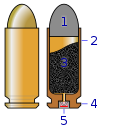
\includegraphics[width=0.5\linewidth]{images/Cartridge_cross_section} 

}

\caption{Image of bullet structure. 1 indicates the bullet, 2 indicates the cartridge casing, 3 indicates the powder, 4 indicates the head of the cartridge casing, and 5 indicates the primer.}\label{fig:structure}
\end{figure}

The practice of bullet matching is based on the concept that rifling in a gun barrel can produce uniquely identifying marks on bullets fired from the gun, due to random variation (PCAST, 2016, p. 104).
\authorcol{Rifling is defined as the spiral ridges in a gun barrel that stabalize the bullet, as shown in Figure} \ref{fig:rifling} \authorcol{, from} baku13 (2005).
\authorcol{The raised areas are known as lands, while the depressed areas are known as grooves.}

\begin{figure}

{\centering 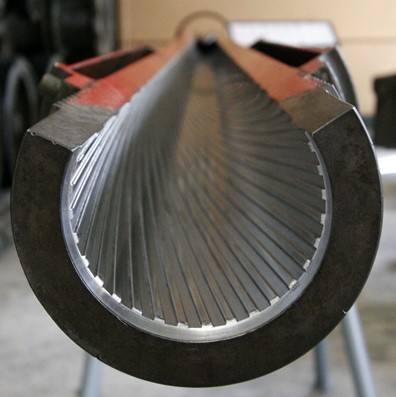
\includegraphics[width=0.5\linewidth]{images/rifling} 

}

\caption{Cross section of a gun. The rifling is the spiral pattern of lands (raised portions) and grooves (indented portions).}\label{fig:rifling}
\end{figure}

\authorcol{When a bullet is fired, it travels down the gun barrel and marks from the rifling are scratched into the bullet's surface.}

\authorcol{This results in indented areas that correspond to the land impressions, as shown in Figure} \ref{fig:fired} \authorcol{, provided by} Gremi-ch (2009).

\begin{figure}

{\centering 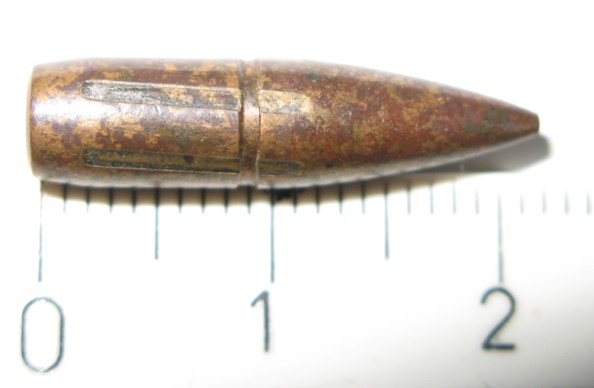
\includegraphics[width=0.5\linewidth]{images/fired_bullet} 

}

\caption{Fired bullet. Indented portion correspond to the gun lands.}\label{fig:fired}
\end{figure}

\authorcol{The diagram in Figure} \ref{fig:fireddiagram} from Hare et al. (2017) \authorcol{demonstrates the structure of these land and groove impressions on a bullet.}
\authorcol{As there are multiple lands on a gun barrel, this results in multiple land impressions on a fired bullet.}

\begin{figure}

{\centering 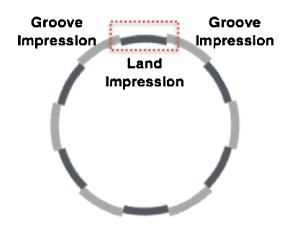
\includegraphics[width=0.5\linewidth]{images/bulletdiagram} 

}

\caption{Fired bullet. Indented portion correspond to the gun lands.}\label{fig:fireddiagram}
\end{figure}

\authorcol{Striation marks, or scratches in the bullet surface caused by the rifling, can be seen on these land impressions, as shown in Figure} \ref{fig:firedland} \authorcol{(provided by} Hare et al. (2017)).
\authorcol{Firearms examiners can compare these striation marks across bullets in order to determine if they were fired from the same gun.}

\begin{figure}

{\centering 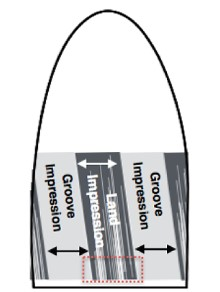
\includegraphics[width=0.5\linewidth]{images/bulletland} 

}

\caption{Fired bullet. Indented portion correspond to the gun lands.}\label{fig:firedland}
\end{figure}

\authorcol{Firearms examiners use comparison microscopes, such as} Figure \ref{fig:microscope}, \authorcol{to compare these striation marks between two bullets, shown in the top right of the figure.}

\begin{figure}

{\centering 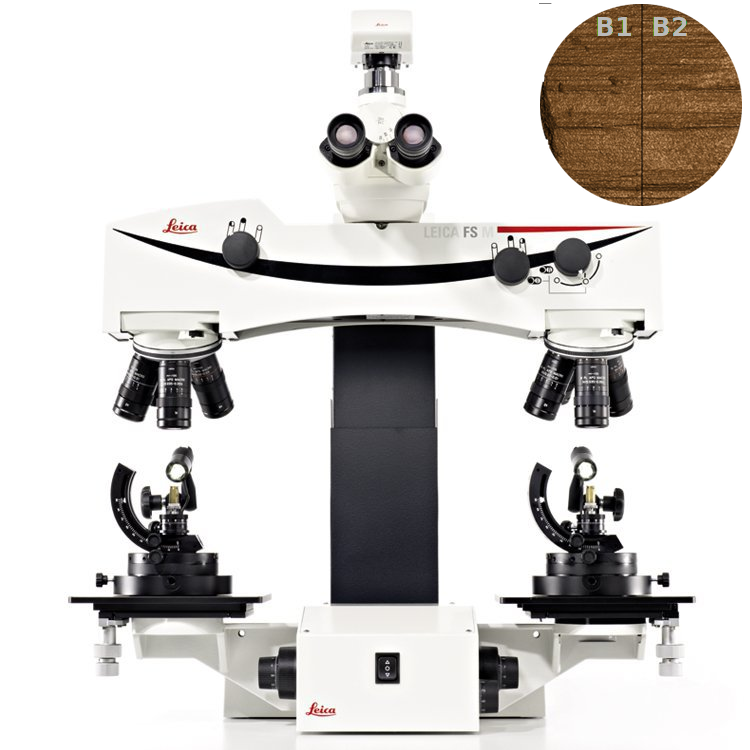
\includegraphics[width=0.5\linewidth]{images/microscope} 

}

\caption{Image of a comparison microscope and aligned bullets}\label{fig:microscope}
\end{figure}

An early attempt to distinguish guns based on the rifling can be found in two issues of ``The Saturday Evening Post'' from 1925, in an article entitled ``Fingerprinting Bullets''.
Stout describes the wrongful conviction and subsequent exoneration of Stielow, who was accused of murder (Stout, 1925a).
At the trial where Stielow was found guilty, an expert for the prosecution stated that there were nine abnormalities on Stielow's gun that corresponded with marks on the fired bullet (Stout, 1925a, p. 7).
It was later found that the bullet found at the crime scene indicated the gun was missing a land -- leaving a distinctive pattern -- while the alleged gun showed no such evidence; the alleged gun also showed evidence of not being fired in more than 3 years (Stout, 1925a).
While this trial did not require `uniquely identifying' marks to rule out the alleged weapon (only a mismatch in lands), it motivated Charles Waite to attempt to catalog the manufacturing methods of guns by various companies around the country, with the goal of connecting a gun to its manufacturer.
Waite soon encountered issues due to the multitude of guns produced abroad, as well as ``cheap knock-offs'' with no clear record, making it difficult to trace a gun or bullet to its manufacturer (Stout, 1925b).
While Waite's early attempt to match barrel markings to specific gun brands was focused on the creation of a `database', more recent firearms identification methods have relied on the direct comparison of bullets, such as comparing fired evidence to a suspected gun.

\hypertarget{issues-in-pattern-analysis}{%
\section{Issues in Pattern Analysis}\label{issues-in-pattern-analysis}}

\hypertarget{subjectivity-of-comparisons}{%
\subsection{Subjectivity of Comparisons}\label{subjectivity-of-comparisons}}

One of the issues listed in the article still resonates today: disagreement among experts; this can be especially problematic in countries that use the adversarial judicial system, where experts can testify on the side of the prosecution or the defense (Stout, 1925a, p. 6).
\authorcol{This could lead to multiple experts with differing conclusions on the same comparison, and are not guaranteed to be unbiased.}
Because there is no quantitative score describing the strength of a bullet match, it is possible for experts to use different criterion when making a conclusion about the same evidence.
Disagreement among experts concerning strength of evidence can be found within a single lab, where experts undergo the same training, use the same equipment and operate under the same procedures, as demonstrated by Montani, Marquis, Egli Anthonioz, \& Champod (2019).
Montani et al. (2019) discuss the importance of independent verification, and how to present results when experts do not agree.
They suggest that, when experts disagree, a third expert should be consulted, and all conclusions should be documented and presented as evidence.
In the case of bullet comparison studies, researchers ask examiners to make conclusions regarding the comparison of several bullets or cartridge cases, and experts do not always agree.
NRC (2009) states that subjectivity is involved in determining ``sufficient agreement'' among firearms (NRC, 2009, p. 155).
This issues is also reflected in Imwinkelried (2020), who suggest that bullet identification is based more on personal experience than on the scientific method.
In plain terms, there is not a set standard for what constitutes sufficient agreement between compared evidence.

Procedural issues may also lead to differing expert opinions across laboratories; one system may not allow an exclusion to be documented if the class characteristics match, while another system may not have such a limitation (Baldwin, Bajic, Morris, \& Zamzow, 2014, p. 6).
In their study, this led to 45 of 218 examiners labeling all different source comparisons as inconclusive, and 96 examiners labeling none of the comparisons as inconclusive (Baldwin et al., 2014, p. 16).
Without a standardized procedure, experts \authorcol{may} evaluate the evidence similarly when comparing two bullets, but must draw different conclusions based on the procedures of their laboratory.
This results in inconsistencies in results based on location, which are compounded with inconsistencies that may arise due to the subjectivity of bullet comparisons.

Aside from the difference in evaluation, subjectivity can lead to bias in pattern recognition.
The need for an unbiased method of evaluation is aptly demonstrated by the case of the Madrid bombing, in which the FBI incorrectly matched a latent fingerprint to the incorrect individual, despite the use of a verification process (Stacey, 2005).
The individual incorrectly identified was a Muslim from Oregon who had been on an FBI watch list (Kassin, Dror, \& Kukucka, 2013, p. 42).
Kassin et al. (2013) suggest that this incorrect conclusion may relate to confirmation bias, and outline other contributing factors, such as extraneous details, external pressures, and order of presentation.
While this example is based on fingerprint analysis, the same issues of subjectivity are present in bullet matching.

Research has been conducted to better understand the factors that drive firearms examiners to make their conclusions.
The use of virtual comparisons allowed Chapnick et al. (2021) to investigate what examiners considered important when evaluating cartridge cases by including a feature to highlight important aspects of comparisons.
They found that examiners generally tended to highlight the same features when making match conclusions (Chapnick et al., 2021, p. 8).
However, not all examiners who correctly identified the samples used `irregularly shaped marks' to distinguish the known matches: the number was around 60\%-70\% (Chapnick et al., 2021, p. 6).
This is far from a unanimous consensus on important features for determining a match in this type of firearm evidence.

While there are issues in subjective bullet matching, there have been attempts to quantify the method.
Biasotti (1959) suggests that statistical methods can be used in order to determine whether two bullets were fired from the same gun.
He concludes that evaluation of individual striation marks \authorcol{(or striae)} is not sufficient, but counting the number of consecutively matching lines may provide enough information to distinguish between matching and non-matching bullets, in the case of the .38 Special Smith and Wesson revolvers used in this study (Biasotti, 1959, p. 37 -- 47).
Biasotti (1959) hoped that such methods may lead to a statistical model for evaluating firearms (47).
The idea of consecutively matching striae (CMS) was addressed again in S. G. Bunch (2000), but a completely standardized or quantifiable method of examination has yet to be developed.
According to Weller (2021), consecutively matching striae is still used today by some examiners (pg 48). However, the use of consecutively matching striae has not been nationally adopted.
Biasotti (1959)'s idea of using consecutively matching lines is used and extended in the bullet matching algorithm developed by Hare et al. (2017).

\hypertarget{scientific-validity}{%
\subsection{Scientific Validity}\label{scientific-validity}}

In recent years, the scientific validity of many forensic science methods have been called into question, as shown in the NRC (2009) and PCAST (2016) reports on feature comparison methods.
General concerns in both reports include foundational evidence for scientific validity, general inability to determine error rates for conclusions, and subjectivity in analysis methods.
Some issues outlined by PCAST (2016) are the circular nature of the identification guidelines \authorcol{put forth by the Association of Firearm and Tool Mark Examiners (AFTE)} and the lack of appropriately designed error rate studies {[}104{]}.
AFTE defines sufficient agreement as ``\ldots the examiner being convinced that the items are extremely unlikely to have a different origin'' (PCAST, 2016, p. 104).
Thus, items are classified as having sufficient agreement if they agree sufficiently enough to conclude that they did not come from different sources.
This guideline is in itself subjective - there are no benchmarks for determining what one means by ``extremely unlikely to have a different origin''.
Both NRC (2009) and PCAST (2016) suggest a move away from subjective methods.
PCAST (2016) states the importance of the development of an objective method for firearms comparisons (113).

These reports also highlighted the lack of studies that produced accurate error rates due to several issues, such as the reporting of inconclusive decisions as well as simple design issues (PCAST, 2016, p. 104 - 112).
For example, Chapnick et al. (2021)'s report does not include inconclusive results as a potential source of error.
They reported three errors (false positives) in their study, and reported a false negative error rate of 0\%, ignoring the wide range of inconclusive decisions.
For known matches of participants from the US and Canada, 38 of 491 comparisons were reported as inconclusive, while 254 of 693 comparisons were reported as inconclusive for know non-matches (Chapnick et al., 2021, p. 6).
The issues of error rate calculation are addressed by Hofmann, Vanderplas, \& Carriquiry (2021), particularly with regards to whether or not inconclusive decisions are treated as errors in calculations.
They suggest to not consider inconclusive decisions errors for the calculation of examiner error rates, used in the lab setting; but to consider inconclusive decisions as errors for process error rates, used for determining if the evidence is relevant enough for judging the guilt of the suspect.
This distinction would allow an examiner to report an inconclusive finding without a negative reflection on their work, as inconclusive decisions are sometimes necessary.
But it would also provide jurors with relevant information in terms of evaluating the reliability of firearms evidence.

In another evaluation of inconclusive results, Dror \& Scurich (2020) describe different ways in which inconclusive results are produced.
They differentiate between inconclusive decisions based on the amount of evidence present; an examiner reaching an inconclusive decision when there is not sufficient evidence to reach a conclusion would be correct, whereas an examiner reaching an inconclusive decision when there is sufficient evidence to reach a conclusion would be incorrect.
This definition relies on a quantifiable amount of evidence necessary to reach a conclusive decision.
By failing to distinguish between correct and incorrect inconclusive decisions in research studies, examiners may opt for the inconclusive choice on hard conclusive comparisons, resulting in error rates that are only valid for easy comparisons when inconclusive decisions are not considered an error(Dror \& Scurich, 2020, p. 336).
Dror \& Scurich (2020) would consider those inconclusive choices to be ``incorrect'' - there is enough evidence to reach a conclusion.
Similarly, another potential error would be the examiner reaching a conclusive decision when there is not sufficient evidence to reach a conclusion (Dror \& Scurich, 2020, p. 334).
This delineates conclusion and errors into distinct categories, which are not seen in error rate studies.
Both inconclusive and conclusive results for the same analysis cannot be correct -- there either is enough evidence to make a conclusion, or there is not enough evidence to make a conclusion; to say otherwise may deflate actual error rates (Dror \& Scurich, 2020, pp. 334--335).
Dror \& Scurich (2020) indicate that this inconclusive issue is more prominent in studies than in casework, as inconclusive decisions are more common in error rate studies.
However, this distinction between correct and incorrect decisions are not commonly made in studies due to a lack of a quantifiable method for separating the two categories, leading to inconclusive decisions contributing lowering the error rate in some studies.

Other issues in the computation of error rates include the use of closed set studies, which result in significantly lower rates of inconclusive decisions and false positives (PCAST, 2016, p. 109). In closed set studies, the source gun is always present, and examiners are asked to match a set of known bullets to a set of unknown bullets - allowing for them to use a process of elimination to make matches; conversely, open set studies do not include all source guns (PCAST, 2016, pp. 108--110).
The Ames Laboratory study is described by PCAST (2016) as an appropriate closed set black-box study (111).
These types of analyses are classified as black-box studies because reported match results are based on an examiner's subjective opinion rather than a list of objective steps (PCAST, 2016, p. 5).
When comparing closed-set studies to non closed-set studies, PCAST (2016) found that closed-set studies had a much lower rate of inconclusive decisions as well as false positives (111).

\hypertarget{scale-of-conclusions}{%
\subsection{Scale of Conclusions}\label{scale-of-conclusions}}

This debate regarding scientific validity continues to this day, as Vanderplas, Khan, Hofmann, \& Carriquiry (2022) shows.
In this declaration, they discuss the current issues with error rate studies, in which they conclude that, until valid error rate studies have been conducted, they cannot support the use of firearms analysis in the courtroom (Vanderplas et al., 2022, p. 10).
Others have called to scale back conclusions that attest to ``individualization'' in the courtroom due to the inability to tie a specific piece of evidence to a specific source, to the exclusion of all other sources (Imwinkelried, 2020; NRC, 2009).
There has been some resistance to scaling back conclusions, however, as demonstrated in a memo sent out by Jim Agar II, an FBI attorney.
They stated that less conclusive language would not be truthful on the part of the firearm expert and to ask firearms examiners to use this language would result in perjury (Agar II, 2021), despite the reliance on subjective methods with unclear error rates.

There has also been some push back against the conclusions of PCAST (2016), as shown in OSAC (2016) (provided by the Firearms and Toolmarks subcommittee.
According to Davis \& Baker (2014), the Organization of Scientific Area Committees (OSAC) subcommittees are ``generally composed of 70\% practitioners, 20\% researchers, and 10\% research and development technology partners and providers''.
OSAC (2016) argue that a false positive error rate is not necessary for determining foundational validity, and that closed set error rate studies are fine for calculating error rates.
OSAC (2016) also suggests that PCAST (2016) ignores the importance of peer review in studies that instruct firearms examiners to work alone, and that black box studies may not properly reflect casework.
However, in order to accurately represent casework, blind testing (where the examiner does not know they are being tested) would be needed - but due to logistical issues and case load, this may not be feasible (PCAST, 2016, p. 59).
OSAC (2016) argues that AFTE language is not circular - the basis of a practical impossibility is based on knowledge of best known non-matches conveyed through training.
Here decisions are based on ``knowledge and experience'', which does not counteract the subjective nature of this decision making.
Despite these disagreements OSAC (2016) also promotes the use of more objective methods.

These differing views are represented in Swofford \& Champod (2022).
Swofford \& Champod (2022) interviewed 15 individuals with a range of expertise in forensic science and the court system in order to assess their feelings about the use of algorithms and the presentation of probabilistic reporting, as opposed to categorical reporting and traditional analysis methods.
They found that prosecutors interviewed supported the use of match terms such as ``identification'' and ``individualization'' instead of probabilistic terms, but two of the prosecutors also rejected the use of terms that convey ``absolute certainty'' (7).
All participants felt that that examiner testimony should accurately reflect scientific limitations, although there was not a consensus on whether this practice was in fact followed in the courtroom - defense attorneys felt that the examiners usually do not uphold this expectation, while lab managers expressed frustration on the part of the court (19).
The scale to which firearm evidence is used in the courtroom is rather contentious, and views may differ based on occupation.

In general, individuals want to guarantee that the information presented in the courtroom is accurate and valid, without causing too much imbalance between the limitations and the categorical conclusion.
However, there isn't agreement on where the balancing point between these two factors are - somewhere between giving too much credit with a match of ``absolute certainty'', and introducing unfounded reasonable doubt by overstating the limitations.
If accurate numerical information on error rates or an objective method of evaluation that can be described to the court were available, it may be possible to have factual statements of limitations and scope of evidence that both sides of the argument would find satisfactory.

Quantifying both the limitations in terms of error rates and the analysis method with set cutoffs would leave the language used by experts when presenting evidence as a variable that can be manipulated.
While there is much debate over the language used in these conclusions, Garrett \& Mitchell (2013) found that the specific language used to describe the strength of the match (when a match was present) had little effect on participants' judgement of guilt. They tested 11 different forms of match language, such as `individualization', `match', or `very likely that the defendant was the source', as well as language that included match conclusions `bolstered' by certainty or likelihood language (Garrett \& Mitchell, 2013, p. 489).
McQuiston-Surrett \& Saks (2009) also found that there was not a significant difference in participants' view of the likelihood the defendant committed the crime when the examiner presented the conclusion as a `match' compared to presenting the conclusion as `similar in all microscopic characteristics.'
Garrett \& Mitchell (2013) suggests that this lack of difference may relate to the overall view of firearms evidence as reliable, meaning that even a weak match basically boils down to being a match in the eyes of the participants (507).
They also found some tempering effect of the expert admitting the possibility that their conclusion was made in error (507).
Thus, the use of accurate error rates may moderate the reliability of experts for a more considered weighing of evidence.
In fact, in the Ninth Judicial Circuit Court, there are jury instructions regarding the need for juries to treat firearms and other `expert' testimony in the same manner as other opinion testimony, in which they must decide how much weight the testimony should receive (United States Courts for the Ninth Circuit, 2019). United States Courts for the Ninth Circuit (2019) also suggest to avoid labelling such testimony as expert testimony, since it may cause jurors to give the testimony undue weight.
One way to fix these issues of subjectivity is by developing a more objective method of evaluation.
One objective method introduced to the forensic sciences is bullet matching algorithms, such as the one described in Hare et al. (2017).

\hypertarget{quantitative-methods}{%
\section{Quantitative Methods}\label{quantitative-methods}}

\hypertarget{bullet-matching-algorithm}{%
\subsection{Bullet Matching Algorithm}\label{bullet-matching-algorithm}}

This bullet matching algorithm was developed by Hare et al. (2017) and uses a random forest in order to determine a match score (Hare et al., 2017, p. 2352).
This algorithm can be described as follows:

The algorithm first takes a 3D scan of the two bullet lands, then identifies a cross section, or a stable area of the bullet land that can be used in comparison.
This cross section is used in order to identify the signatures of the bullets, or a 2D line that captures the marks scratched onto the bullet's surface.
First the shoulders (the raised area on either side of the scratched pattern) must be removed from the cross section.
Then a loess smoothing is applied twice in order to remove the curvature of the bullet.
What is left is the bullet land's signature (which will show the peaks and valleys produced by the barrel of the gun).
The two signatures are compared using a variety of attributes, such as consecutively matching striae and the relative height of the peaks/valleys, as shown in Figure \ref{fig:signaturecompare}.

\begin{figure}

{\centering 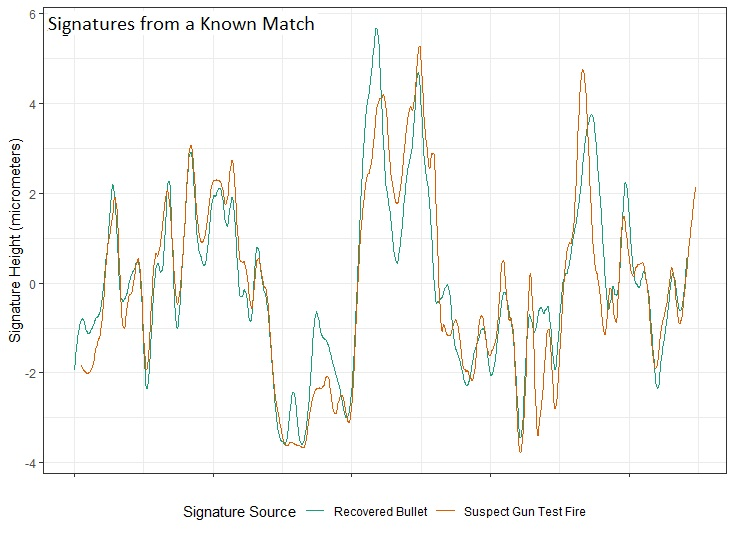
\includegraphics[width=0.49\linewidth]{images/Match_Signatures} 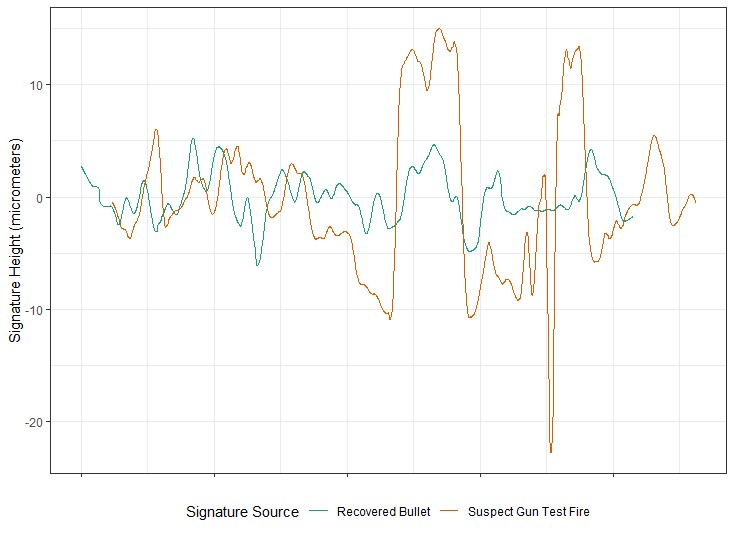
\includegraphics[width=0.49\linewidth]{images/K995_NoMatch_Signatures} 

}

\caption{Left image depicts two matching signatures, while the right image depicts two non-matching signatures.}\label{fig:signaturecompare}
\end{figure}

A random forest is used to compare the two signatures and come up with a match score for the lands.
Lands are then aligned across the bullet for the maximal random forest score, and this number would be considered the match score for the bullet.
Figure \ref{fig:gridcompare} shows two grids of land match scores computed in two different bullet comparisons.

\begin{figure}

{\centering 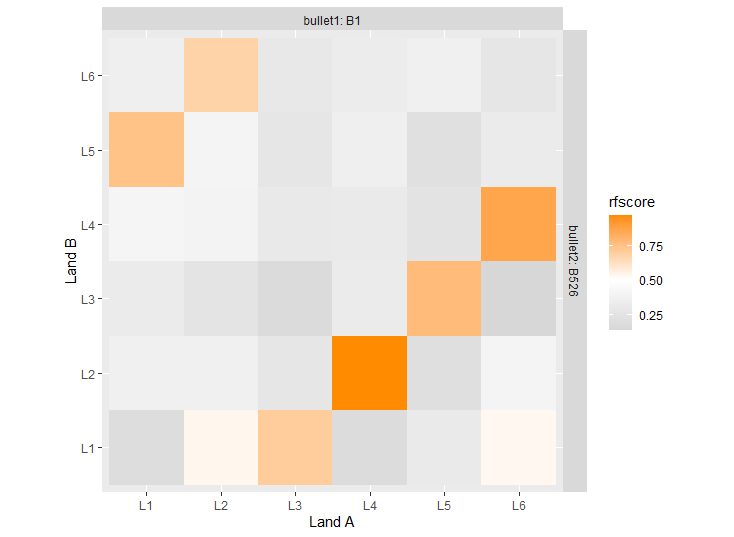
\includegraphics[width=0.49\linewidth]{images/F526_Match_SingleGrid} 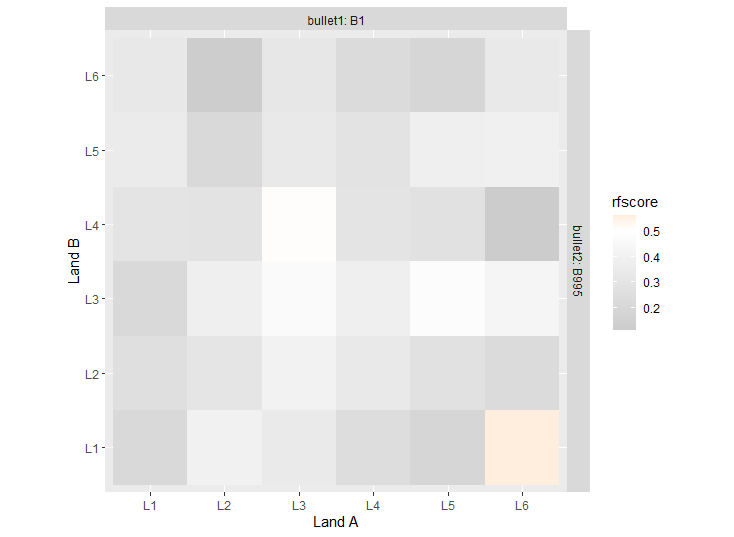
\includegraphics[width=0.49\linewidth]{images/K995_NoMatch_SingleGrid} 

}

\caption{Left image depicts two matching bullets (indicated by high land-to-land match scores in a diagonal formation), while the right image depicts two non-matching bullets.}\label{fig:gridcompare}
\end{figure}

In multiple tests, it was found that the algorithm is able to successfully distinguish between known matches and known non-matches without the use of an inconclusive decision (Vanderplas, Nally, Klep, Cadevall, \& Hofmann, 2020, p. 10).
If the bullet is not fit for algorithmic comparison, then an `inconclusive' result may still be reached.
This may be the case for gun types that have not been tested for the algorithm.
The use of an algorithm allows for quantification of bullet matching, for cases where the algorithm has been verified.

There are some concerns about implementing algorithms for forensic evidence in the courtroom, due to the issue of explaining complex methods to jurors.
In a similar combination of computerized results and human interpretation, Montani et al. (2019) suggest presenting the algorithm as a ``second independent expert'' whose comparison and conclusion can be compared to and presented alongside the examiner's.
Supplementing the decision of the forensic expert with an algorithm would allow for verification of results in two independent methods.
The three laboratory managers interviewed by Swofford \& Champod (2022) suggested using algorithms as a supplement to the forensic examiner (6), similar to Montani et al. (2019)'s suggestion.
The three prosecutors varied in their feelings of algorithms in the courtroom: one thought that they would add unnecessary complications, while two suggested that the algorithms may be useful for the forensic expert (Swofford \& Champod, 2022, p. 8).
The three defense attorneys, as well as the three judges, also supported the use of algorithms as empirical evidence, while stating concerns of transparency (Swofford \& Champod, 2022, pp. 10--13).
Three academic scholars supported the use of algorithms, so long as the algorithms can be understood, have been validated, and do not include factors that may cause systematic biases (Swofford \& Champod, 2022, p. 16).
Swofford \& Champod (2022)'s study demonstrates the variety of opinions on algorithm implementation throughout forensic science, although most support the use of algorithms.

\hypertarget{quantitative-results}{%
\subsection{Quantitative Results}\label{quantitative-results}}

Quantitative methods of examination can lead to quantitative results.
In this case, the quantitative results are in the form of a match score, but in other cases, results may be presented as a likelihood ratio.
For example, John Song, Chen, Vorburger, \& Soons (2020) proposed a likelihood approach for a cartridge case comparison method that uses congruently matching cells.
This is a change from the match language usually used by forensic examiners, but these likelihood ratios may have some benefit.
Marquis et al. (2016) suggest that the use of a likelihood ratio requires examiners to consider what they are including when weighing the strength of evidence, and provides a value that can be consistent across disciplines (4).
This quantitative approach, even while conducting a subjective evaluation, is meant to prevent examiners from being biased by information provided outside of their direct examination (S. Bunch \& Wevers, 2013, p. 223).
The approach also asks examiners to consider both the null and alternative hypotheses, and may make it less likely for either the examiners or jurors to transpose the conditional, which may happen in the case of reporting probabilities (Evett, 1998; Marquis et al., 2016, p. 3).

As an example of transposing the conditional, suppose an examiner were comparing a bullet from the suspect's gun to a bullet recovered from the crime scene.
The examiner may find that there is significant agreement between the two bullets.
They may then conclude that ``the probability of seeing such significant agreement between the two bullets \emph{given that another gun fired the bullet at the crime scene} is small''.
In this case, the examiner is making a statement regarding the amount of agreement between the two bullets (P(Correspondence\textbar Different Source)).
If the conditional is transposed, the statement would become ``the probability that another gun fired the bullet at the crime scene \emph{given the significant agreement between the two bullets} is small'' (P(Different Source\textbar Correspondence)).
Here, the conditional part of the statement has been switched, so that the examiner is making a statement regarding the gun being fired at the crime scene instead of a statement with regards to the bullet comparison.
By stating a likelihood ratio, such as ``the bullet comparison provides strong support for the proposition that the two bullets came from the same gun rather than the proposition that the two bullets came from different guns'', both the null and alternative hypothesis are clearly stated, and the focus of the statement is on the bullet comparison, rather than the gun's presence at the crime scene.

As shown above, the likelihood ratio directly compares the null and alternative hypotheses in a case, which is not accomplished by considering a single probability (Nordgaard, Ansell, Drotz, \& Jaeger, 2012, p. 6).
Likelihood ratios also allow for the integration of evidence from multiple sources, and individual likelihood ratios may be multiplied together to calculate an overall likelihood ratio.
Meuwly, Ramos, \& Haraksim (2017) suggested guidelines for validating both score- and feature-based likelihood ratio methods, so this form of result presentation could be more widely accepted.
These methods included validation criteria for all variables considered in a likelihood ratio, where validation criteria can be considered in several ways: a comparison with current ``state of the art'' methods, detection error trade-off graphs to measure discriminating power, and performing validation on a validation data set.

\hypertarget{explainability-in-the-courtroom}{%
\subsection{Explainability in the Courtroom}\label{explainability-in-the-courtroom}}

One roadblock in the use of quantitative methods and results, such as likelihood ratios, in the forensic sciences is the necessity to explain such methods to jurors so that they can understand the method and results well enough to make informed decisions in court cases.
Association of Forensic Science Providers (2009) stated that opinions and conclusions should be expressed in likelihood ratios when outlining guidelines for forensic experts (163).
Participants in Swofford \& Champod (2022) expressed concern that probabilistic reporting (as opposed to categorical reporting) would be confusing and easily misinterpreted, when compared to the alternative of categorical reporting (18).
In order to gauge how quantitative methods are perceived in the courtroom, we can consider fingerprint and DNA analysis.
Garrett, Mitchell, \& Scurich (2018) studied the use of FRStat for fingerprint matching in the courtroom.
The FRStat language presented to the study participants is as follows: ``The probability of observing this amount of correspondence is approximately {[}XXX{]} times greater when the impressions are made by the same source rather than by different sources'' (language from Defense Forensic Science Center, 2018).
Garrett et al. (2018) used ratios from 10 times greater to 100,000 times greater, and found that the likelihood that the subject committed the crime according to the participants did not change significantly.
This demonstrates that potential jurors may have trouble accurately interpreting statistical results, including likelihood ratios.

In DNA research, Koehler (2001) found that participants were more likely to believe the subject was the source of the DNA when presented with a probability instead of a frequency.
When asked about how many individuals would match DNA for a given match proportion in a population of 500,000, 60.7\% of participants who received a frequency and 42.1\% of individuals who received a probability answered correctly (Koehler, 2001, p. 503).
When asking these individuals to determine the guilt or innocence of a suspect, the percentage of participants who correctly interpreted the DNA results seems relatively low.
Jurors are also prone to find evidence to be weaker when frequencies are presented as whole number (1 out of 100,000) compared to a decimal number (0.1 out of 10,000), even though the frequencies represent the same value (Koehler \& Macchi, 2004, p. 544).
These studies show that individuals struggle with interpreting numerical results, and assigning appropriate weight to likelihood ratios.

In addressing these issues of interpretation, attempts have been made to assign a verbal scale to be used alongside a likelihood ratio, such as the European recommendations for reporting forensic science \authorcol{put forth by the European Network of Forensic Science Institutes} (ENFSI, 2016).
A sample of phrasing from their recommended scale has been recreated in Table \ref{tab:enfsi}.
Verbal values range from no support to extremely strong support, and correspond to a numerical output.
This type of scale would present jurors with both the quantitative result as well as a brief interpretation, so they are not solely relying on their own perception of what the likelihood ratio qualitatively means.
It also offers a numerical scale that may encourage consistency across examiner reports.

\begin{longtable}[]{@{}
  >{\centering\arraybackslash}p{(\columnwidth - 2\tabcolsep) * \real{0.2016}}
  >{\centering\arraybackslash}p{(\columnwidth - 2\tabcolsep) * \real{0.7984}}@{}}
\caption{\label{tab:enfsi} Sample language from ENFSI (2016) (17)}\tabularnewline
\toprule()
\begin{minipage}[b]{\linewidth}\centering
Likelihood Ratio
\end{minipage} & \begin{minipage}[b]{\linewidth}\centering
Verbal Equivalent
\end{minipage} \\
\midrule()
\endfirsthead
\toprule()
\begin{minipage}[b]{\linewidth}\centering
Likelihood Ratio
\end{minipage} & \begin{minipage}[b]{\linewidth}\centering
Verbal Equivalent
\end{minipage} \\
\midrule()
\endhead
1 & The forensic findings do not support one proposition over the other \\
2 - 10 & The forensic findings provide weak support for the first proposition relative to the alternative \\
10 - 100 & \ldots provide moderate support for the first proposition rather than the alternative \\
100 - 1,000 & \ldots provide moderately strong support for the first proposition rather than the alternative \\
1,000 - 10,000 & \ldots provide strong support for the first proposition rather than the alternative \\
10,000 - 1,000,000 & \ldots provide very strong support for the first proposition rather than the alternative \\
1,000,000 and above & \ldots provide extremely strong support for the first proposition rather than the alternative \\
\bottomrule()
\end{longtable}

A similar scale is also suggested by Evett (1998), with verbal values of ``Limited support'', ``Moderate support'', ``Strong support'', and ``Very strong support'' (201).
These values approximately correspond to the scale above, but consists of fewer categories.
Marquis et al. (2016) suggest against providing the full verbal scale to participants, because participants may use other terms on the scale in order to orient the likelihood ratio in comparison to the full scale (7).
However, this ability to orient relative to other values may assist jurors in accurately judging the strength of evidence presented.

While verbal scales are useful for clarification, individuals may not always interpret them consistently.
For example, Budescu \& Wallsten (1985) asked participants to rank common probabilistic words (such are ``rarely'' or ``usually'') on three separate occasions, finding that individuals typically gave consistent rankings across time points, but there was variation in rankings between individuals.
In an earlier study, Lichtenstein \& Newman (1967) asked individuals to assign numerical probabilities to probabilistic words, finding that eight of the eleven mirror terms (such as ``quite likely'' and ``quite unlikely'') demonstrated asymmetry - positive terms (such as likely) scored lower than their mirrored negative terms (unlikely). For example, ``quite likely'' and ``quite unlikely'' had median values of 0.8 and 0.1, respectively (Lichtenstein \& Newman, 1967, p. 564).

Examiners also show evidence of inconsistency in scale interpretation.
Mattijssen, Witteman, Berger, Brand, \& Stoel (2020) asked examiners to use a verbal scale for degree of similarity and support when digitally comparing cartridge cases.
When using a verbal scale for degree of similarity/support, Mattijssen et al. (2020) found that the between-subject and within-subject reliability was moderate to high (11).
Mattijssen et al. (2020) asked 10 examiners who regularly used likelihood ratios to provide both a verbal degree of support along with a likelihood ratio.
They found that the verbal degrees of support were in general an overestimation when compared to the likelihood ratios (8).
While this is a small non-representative sample, it suggests that verbal scales do not always correspond to quantitative scales across subjects.
By combining the quantitative analysis with a verbal translation, it may be possible to present quantitative results in a manner that is understood consistently by laypeople.

This mix of quantitative language alongside more categorical terms is supported by subjects in Swofford \& Champod (2022).
Almost all participants expressed concerns about the interpretation of the probabilistic language, and many recommended a combination of both methods (Swofford \& Champod, 2022).
The prosecutors interviewed thought that match language was sufficient by itself, and did not wish to complicate testimony with probabilistic language (Swofford \& Champod, 2022, p. 8).
McQuiston-Surrett \& Saks (2009) studied the use of match language versus probabilities with both judges and juries.
Both groups assigned higher probabilities to the defendant committing the crime when presented with qualitative evaluation or a single probability for the hair comparison, as compared to frequency methods of reporting.
McQuiston-Surrett \& Saks (2009) found that participants were more sure of the guilt of the defendant when qualitative language was used as opposed to a subjective probability.
While match language may give jurors more confidence, it could have the effect of shifting the consideration of evidence from the jury (who in a quantitative approach would need to determine whether or not they feel a likelihood ratio is large enough to indicate that the subject is the source) to the forensic expert, who can declare a match.

Verbal scales are also often used to record participant responses.
Likert scales can be used to evaluate several factors, such as the reliability, understanding, and scientific quality of the forensics expert, the algorithm, and the testimony in general.
It is therefore important to ensure that participants' views are accurately recorded with Likert type scales, which can vary in the number of categories used.
Several researchers found that the 7-point scale may perform or represent the participants' true views better than the 5-point scale (Finstad, 2010; Joshi, Kale, Chandel, \& Pal, 2015).
Participants often preferred more categories, such as 7, 9, or 10 (Komorita \& Graham, 1965; Preston \& Colman, 2000).
However, Preston \& Colman (2000) found that reliability decreased with more than 10 categories.
This indicates that 7, 9, or 10 point scales should be adequate for reliable responses that accurately represent the participant's views.
Other methods have also been used to evaluate participant responses, such as asking participants to give a likelihood ratio or a probability of guilt.
Thompson, Kaasa, \& Peterson (2013) asked participants rate the chance of guilt on a scale from: 1 chance in 1 trillion he is guilty, to 999,999,999,999 chances in a trillion that he is guilty, with impossible to be guilty and certain to be guilty as the most extreme values.
They compared results from participants to Bayesian conditional probabilities based on provided likelihoods of a match and error rates in order to consider how much weight participants were giving DNA evidence.

\hypertarget{demonstrative-evidence}{%
\subsection{Demonstrative Evidence}\label{demonstrative-evidence}}

Aside from result language or scales used, another important factor in jury decision making is demonstrative evidence.
Images can supply helpful context in describing complex forms of analysis, but they may also introduce bias in the form of ``truthiness'', a\authorcol{n official} term introduced by comedian Stephen Colbert.
He described truthiness as the quality of something \emph{seeming} true (Colbert, 2005).
In this video, Colbert talks about ``thinking with your head vs.~knowing with your heart'', where some information may feel true, regardless of the facts.
Bornstein \& Greene (2011) found a ``truthiness'' effect in the courtroom - jurors tend to remember evidence that align with their previous beliefs (65).
\authorcol{This concept can apply to images that make people more likely to feel like a statement is true, even when they do not contribute new evidence.}
Kellermann (2013) suggests that the truthiness or ``falsiness'' of non-probative visual images should be carefully considered before using images in the courtroom ``\ldots both to prevent backfire effects and to capitalize on every possible tactic that can be used to persuade jurors\ldots{}'' (40).
While the concept of truthiness can be used to benefit either side in an adversarial justice system, trial outcomes should be based on factual evidence, rather than feelings that evidence is factual.
In the case of images in trials, it is important to balance the benefit of providing additional information to the jury via images without increasing truthiness.

The impact of photos on an individual's perception can be rather large, as investigated by Cardwell, Henkel, Garry, Newman, \& Foster (2016).
They asked individuals to ``give'' or ``take'' food from an animal, represented by a word.
Subjects were later asked to identify whether or not they gave food to an animal -- either accompanied by an image or not.
Individuals were more likely to say that they gave food to an animal if it was accompanied by an image (Cardwell et al., 2016, p. 887).
They found that images had an effect for positive associations such as giving food, but not negative associations such as taking food (Cardwell et al., 2016, p. 883).
In this case, the use of images may make it easier for individuals to visualize a scenario (giving food), and thus makes them more likely to remember the event - whether it happened or not.

In a study of perception, McCabe \& Castel (2008) presented a variety of graphics alongside articles relating to cognitive neuroscience.
The graphics all contained the same information, which was already presented the accompanying article.
They found that participants gave higher ratings of scientific reasoning to articles that included a brain image with activated areas, as opposed to a bar chart, topographical brain graphic, or no graphic.
Participants were also more likely to agree with the conclusion of an article when the brain image was present, compared to when it was absent.
Although the information presented in the articles did not change throughout these conditions, the brain image appears to add more ``truthiness'' to the articles, causing individuals to find them more scientific than articles with other graphics or no graphics.

In the courtroom, studies have been conducted to evaluate the effect of images of the brain.
Gurley \& Marcus (2008) studied the use of brain images when arguing the defendant is not guilty by reason of insanity.
In a study on introduction to psychology university students, they found that the inclusion of images showing a brain lesion increased the odds of the participants finding the defendant not guilty by reason of insanity.
MRI scans were presented with additional information regarding impulse control for the damaged area, so the effect may not be caused by the images themselves but rather by the additional information.
Schweitzer et al. (2011) investigated whether images of the brain presented alongside expert testimony with regards to a mental disorder effected the participant's verdict of the defendant's mental state.
In this case, no additional information was provided alongside the neuroimage, allowing the effect of the image itself to be studied.
They found that the inclusion of neuroimages did not significantly effect the judgement of the participants.
The influence of images on individuals remains unclear, and may be situationally dependent.

\hypertarget{conclusion}{%
\section{Conclusion}\label{conclusion}}

In order to ensure that the US justice system is just, we must be confident that the evidence presented in the courtroom is scientifically valid, and that the evidence is presented in a way that gives jurors the ability to appropriately judge its strength.
This includes the use of accurate error rates as well as quantitative responses.
One way to facilitate error rate calculation and quantitative results is through the use of algorithmic or statistical methods.
These methods must, however, be explained in a manner that is understandable to those without a statistical background, while limiting any of the potentially biasing effects of ``truthiness''.

\hypertarget{study1}{%
\chapter{Jury Perception of Bullet Matching Algorithms and Demostrative Evidence}\label{study1}}

\hypertarget{background}{%
\section{Background}\label{background}}

\hypertarget{firearms-examiners}{%
\subsection{Firearms Examiners}\label{firearms-examiners}}

The foundational belief in bullet comparisons as a form of identifying evidence is that guns can leave unique striation marks on a bullet as an artifact of the rifling process (PCAST, 2016, p. 104).
Striation marks are left on portions of the bullets known as ``lands'', due to contact with the rifling as the bullet is fired.
These marks are compared by examiners across bullets in order to identify if bullets were fired from the same source.
These examinations are subjective, as they are based on the firearms examiner's experience and judgement (NRC, 2009, p. 153).
This can lead to issues of bias in analysis (Kassin et al., 2013). In 2019, the PCAST report highlighted common issues with traditional bullet matching methods, such as the lack of appropriately designed error rate studies and the circular nature of AFTE's bullet matching guidelines (PCAST, 2016, pp. 104--112).
Issues in error rate studies have been discussed in several articles (Dror \& Scurich, 2020; Hofmann et al., 2021).
PCAST emphasizes the importance of the development of an objective method for firearms comparisons (PCAST, 2016, p. 113).
The use of an automatic, objective method would contribute to quantifiable presentation of evidence and would lower the effort required to identify the method's error rate.

\hypertarget{bullet-matching-algorithm-1}{%
\subsection{Bullet Matching Algorithm}\label{bullet-matching-algorithm-1}}

Following PCAST's publication, many methods of statistical matching have been developed and evaluated, such as Hare et al. (2017), Vanderplas et al. (2020), J. Song et al. (2012), and Vorburger, Song, \& Petraco (2015).
In this study, the bullet matching algorithm used was developed by Hare et al. (2017).
The algorithm can briefly be described as follows:

\begin{enumerate}
\def\labelenumi{\arabic{enumi}.}
\tightlist
\item
  A 3D scan is taken of each bullet land (containing striation marks to be compared), a stable cross-section is extracted, and shoulders (without relevant striation marks) are removed, as in \ref{fig:shoulder}, an image from Hare et al. (2017).
\end{enumerate}

\begin{figure}
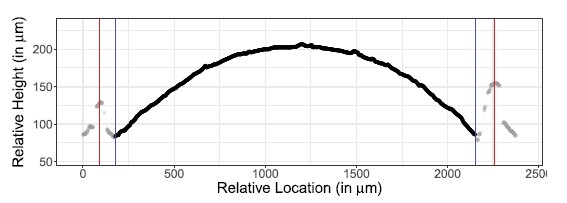
\includegraphics[width=\linewidth]{images/shoulder} \caption{The land is shown in the center. Shoulders are shown outside of the vertical lines.}\label{fig:shoulder}
\end{figure}

\begin{enumerate}
\def\labelenumi{\arabic{enumi}.}
\setcounter{enumi}{1}
\tightlist
\item
  A smoothing function is applied twice in order to extract the signature, a pattern of high and low points on the bullet's surface corresponding to the striation marks.
  The signature can then be compared to land signatures from other bullets, as in \ref{fig:signature}.
\end{enumerate}

\begin{figure}
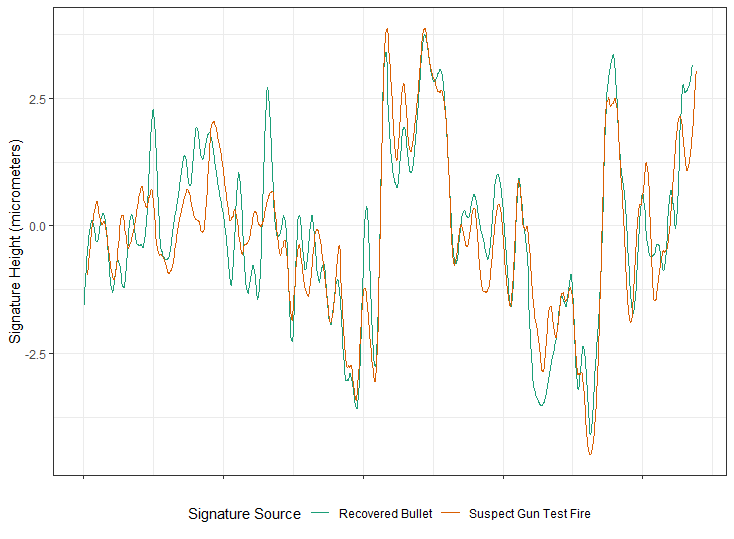
\includegraphics[width=\linewidth]{images/F526_Match_Signatures} \caption{Two aligned signatures for a known match. Image generated from Houston dataset by authors.}\label{fig:signature}
\end{figure}

\begin{enumerate}
\def\labelenumi{\arabic{enumi}.}
\setcounter{enumi}{2}
\tightlist
\item
  Traits, such as consecutively matching striae and depth of grooves, are then used in a random forest to produce a match score (ranging from 0 to 1) for the lands.
  The random forest consists of decision trees that consider a combination of variables and responses in order to predict if two signatures were created by the same gun.
  \authorcol{The decision trees in a random forest each consider a subset of variables and observations to decide whether or not the lands match.}
  The decisions of these trees are combined to produce the match score.
  Lands are then aligned across bullets in order to compute an overall match score for the bullets, as in \ref{fig:grid}.
\end{enumerate}

\begin{Shaded}
\begin{Highlighting}[]
\FunctionTok{include\_graphics}\NormalTok{(}\AttributeTok{path =} \StringTok{"images/Test\_Fire\_F526.jpeg"}\NormalTok{)}
\end{Highlighting}
\end{Shaded}

\begin{figure}
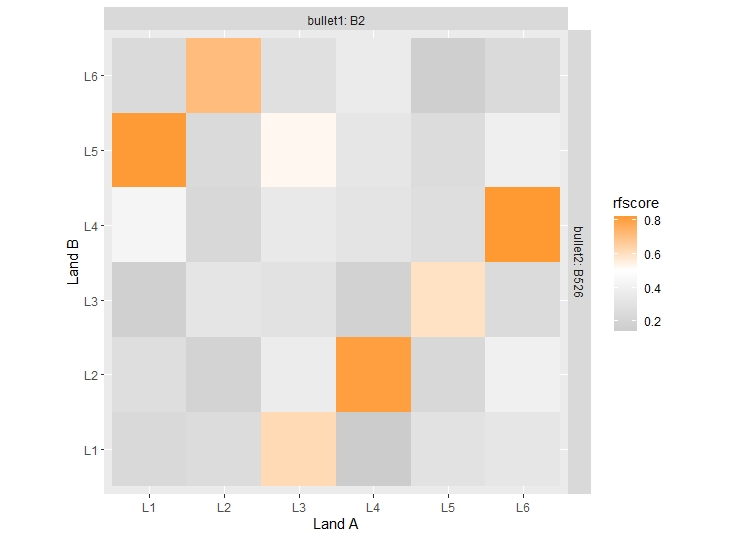
\includegraphics[width=\linewidth]{images/Test_Fire_F526} \caption{Diagonal correspondence (in orange) among lands indicate a match, as shown here. Image generated from Houston dataset by authors.}\label{fig:grid}
\end{figure}

This algorithm was trained on Hamby's Consecutively Rifled Ruger Barrel Study data sets 252 and 173 (Vanderplas et al., 2020), and the final random forest was able to correctly predict all matches and non-matches (Hare et al., 2017, p. 2350).
Three sets were then used to verify the algorithm: Hamby set 44, Phoenix PD, and Houston FSC (Vanderplas et al., 2020, p. 5).
The algorithm performed well for undamaged bullets, and was able to completely distinguish between matches and non-matches when a cutoff value was individually chosen for each data set (Vanderplas et al., 2020, p. 10).

\hypertarget{explainable-machine-learning---previous-research}{%
\subsection{Explainable Machine Learning - Previous Research}\label{explainable-machine-learning---previous-research}}

Jurors' ability to interpret statistical methods and language is \authorcol{in doubt}; in a study conducted by Koehler (2001) with regards to the probability of a random match in DNA evidence, they found that jurors had different interpretations when the probability was presented as 1 out of 1,000 versus 0.1 out of 100, where those presented with a decimal number were more likely to view the probability of a random match as smaller.
In another study, Garrett et al. (2018) asked jurors to evaluate evidence that used the following FRStat language, typically used in fingerprint analysis: ``The probability of observing this amount of correspondence is approximately {[}XXX{]} times greater when the impressions are made by the same source rather than by different sources'' (language from Defense Forensic Science Center, 2018).
When asked for the likelihood the defendant committed the crime when presented with the above FRStat language, participants did not provide significantly different likelihoods for values ranging from 10 times greater to 100,000 times greater.
This may demonstrate a lack of understanding when jurors are presented with numerical results for statistical evidence.
ENFSI (2016) proposes a verbal scale to supplement likelihood ratios, which may alleviate some of the burden of statistical interpretation from potential jurors.
This scale ranged from weak support, corresponding to a likelihood ratio between 2 and 10, to very strong support, corresponding to a likelihood ratio greater than 10,000 (ENFSI, 2016, p. 64).
When interviewing judges, lawyers, forensic scientists, and forensic researchers, Swofford \& Champod (2022) found that many expressed concern regarding the interpretation of probabilistic language, and several suggested a combination of both match and probabilistic language.
Hare et al. (2017)'s algorithm differs from previous presentation methods in that its output is a match score, as opposed to a likelihood ratio.
In this study, potential jurors may encounter both the algorithm's match score alongside the categorical match language of the examiner.

\hypertarget{demonstrative-evidence-1}{%
\subsection{Demonstrative Evidence}\label{demonstrative-evidence-1}}

Images are often used to assist individuals in understanding non-image information.
However, images may have an effect of making a scenario more believable, as demonstrated in a study by Cardwell et al. (2016) which involved ``giving'' or ``taking'' food from animals with or without images.
Images are also mentioned as a factor that can influence how truthful individuals view statements in the courtroom - even if no new information is presented through the presence of the image (Kellermann, 2013).
Therefore, the use of images in a courtroom should be studied for an effect with regards to how subjects perceive the evidence presented - namely, if there is a difference in how reliable or credible they feel the experts are, based on the presence or absence of images.
\authorcol{Because the images are intended to aid only in interpretation, we would hope for an increase in understanding across all other conditions, while reliability and credibilty stay the same.}
\authorcol{However, based on previous research, it seems probable that the presence of images would increase the perceived reliability and credibility of the evidence and expert, respectively.}

\hypertarget{methods}{%
\section{Methods}\label{methods}}

\hypertarget{study-format}{%
\subsection{Study Format}\label{study-format}}

\authorcol{First,} participants are presented with a short scenario based on Garrett, Scurich, \& Crozier (2020): a bullet is the only evidence recovered from an attempted convenience store robbery, and is tested against a gun found in Richard Cole's car in a routine traffic stop.
\authorcol{Participants are informed that the court clerk was unable to identify the robber because they were wearing a ski mask, and that the testimony presented represented all relevant information.}
\authorcol{They were also advised that they would be unable to re-read testimony, and a notepad was provided for their convenience.}
Participants are then asked to read a transcript of mock court testimony, and rate their impression of the evidence presented, as well as their impression of the experts.
This document included expert testimony, cross examination, and questions from the jury conveyed through the judge regarding error rates.
\authorcol{The expert testified to their qualificiations, as well as the process of bullet matching.}
\authorcol{They then described comparing the fired evidence to a test fire from the defendant's gun, and the results of the comparison.}
\authorcol{When the algorithm was included, the firearms examiner also described the algorithm's match score resulting from this comparison.}
\authorcol{Cross examination included questions regarding the ability to uniquely identify the source of the bullet, as well as the subjectivity of the comparison.}

\authorcol{When the algorithm was included, an algorithm expert then testified.}
\authorcol{They also listed their qualifications and involvement in the development of the algorithm.}
\authorcol{The expert would then describe the process for obtaining a match score (similar to the algorithm description in the previous section).}
\authorcol{They also spoke to the publication history of the algorithm, the code availability, and the algorithm's applicability to the type of firearm considered in the case.}
\authorcol{Cross examination included questions on the newness of the algorithm, as well as subjective aspects of calibration, and limitations with respect to the types of bullets that it can evaluate.}

The testimony was based on actual court testimony provided by forensics experts lawyers, and judges, shown in Appendix \ref{testimony-transcripts}.

\authorcol{After reading the transcript, participants were directed to respond to some questions regarding the testimony.}
\authorcol{They were first given information about their responsibility as jurors to choose whether or not to convict, and the 'beyond reasonable doubt' threshold was established before asking participants for their conviction decision.}
\authorcol{Participants were also asked to estimate the probability that the defendant committed the crime, and the probability that the gun was involved in the crime.}
\authorcol{These questions were followed by several Likert scales on the strength of evidence, the credibility of the examiners, reliability and scientificity of the evidence, and understanding of the procedures.}

Two attention check questions were asked, in order to ensure that participants were reading both the testimony and the subsequent questions.
The first attention check asked participants to identify the caliber of bullet recovered from the crime scene, while the second attention check asked participants to select a specific value from a Likert scale.

The study includes three \authorcol{independent} variables: \authorcol{presence or absence} of the algorithm, \authorcol{presence or absence} of demonstrative evidence (images), and conclusion (match, exclusion, or inconclusive).
In the case of the algorithm, two testimonies were presented: that of the firearms expert (Terry Smith), and that of the algorithm expert (Adrian Jones).
The firearms expert presented the algorithm results for the case alongside their own analysis, and suggests that the algorithm's results supports their conclusion.
By presenting the algorithm results with the interpretation suggested by the firearms expert, we hoped that potential jurors could use the firearms expert's explanation and conclusion to guide their understanding of the algorithm's results.
The algorithm expert then describes in greater detail the algorithm's process, and its validity for this particular case.
When demonstrative evidence is present, images of rifling (baku13, 2005; Gremi-ch, 2009), a bullet comparison, and algorithm images (such as those shown above) were included alongside the testimony.
In terms of the conclusion: a ``match'' indicated agreement in individual and class characteristics; an ``exclusion'' indicated an agreement of class characteristics, but disagreement in individual characteristics; and an ``inconclusive'' indicated an agreement in class characteristics, but not enough agreement in individual characteristics to state that there was a match.

The number of survey questions that respondents received depended on the scenario; participants who received the algorithm were asked more questions than those who did not receive the algorithm.
For example, participants who did not receive the algorithm were asked about the reliability of the forensics examiner's bullet comparison and the reliability of the field of firearms as a whole.
Those who received the algorithm were asked about the reliability of the forensics examiner's bullet comparison, the reliability of the algorithm's comparison, the overall reliability in the case (which includes both the algorithm comparison and the forensics expert's comparison), as well as the reliability of the field of firearms as a whole.
This same format was used when asking participants about credibility and scientificity.

\hypertarget{prolific}{%
\subsection{Prolific}\label{prolific}}

Participants were recruited using Prolific, an online survey-taking website.
\authorcol{From the Prolific website, participants were directed to a link containing our survey, created using RShiny.}
We selected options to recruit a representative sample of individuals located in the United States, and asked that participants self-screen for jury eligibility before completing the survey.
Jury eligibility was defined as US citizens over the age of majority in their state who had not been convicted of a felony, were not active law enforcement, military, emergency response, or a judge, and who did not have a disability that would prevent them from serving on a jury.
They were also required to have normal or corrected to normal vision, due to the images used in the study.
Participants were compensated with \$8.40 for completing the study, for an hourly compensation rate of about \$27.79 (median completion time of approximately 18 minutes).\\
Individuals who did not include their Prolific identification number and an individual whose notes indicated that they had progressed far enough into the survey to get a separate scenario before restarting were excluded from analysis.

\begin{figure}

{\centering 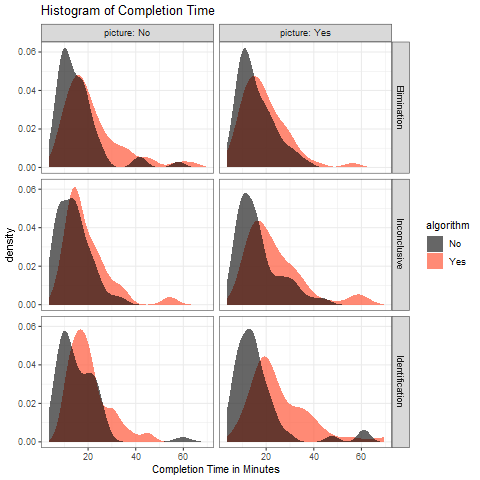
\includegraphics[width=\linewidth]{images/completiontime} 

}

\caption{Completion Time by Condition for all unique fingerprints}\label{fig:completiontime}
\end{figure}

Figure \ref{fig:completiontime} depicts completion times (from completion of the demographics information to the end of the survey) by conditions for unique fingerprints (n=559), excluding 5 observations greater than 75 minutes. In general, it appears that those who received the algorithm condition took slightly more time on average than those who did not (median values of 19.134 minutes and 13.716 minutes, respectively). This is unsurprising, given the increased length of the algorithm condition.

\hypertarget{results}{%
\section{Results}\label{results}}

\authorcol{Due to scale compression, no statistical analysis was performed on this data.}

\hypertarget{participants}{%
\subsection{Participants}\label{participants}}

\begin{figure}

{\centering 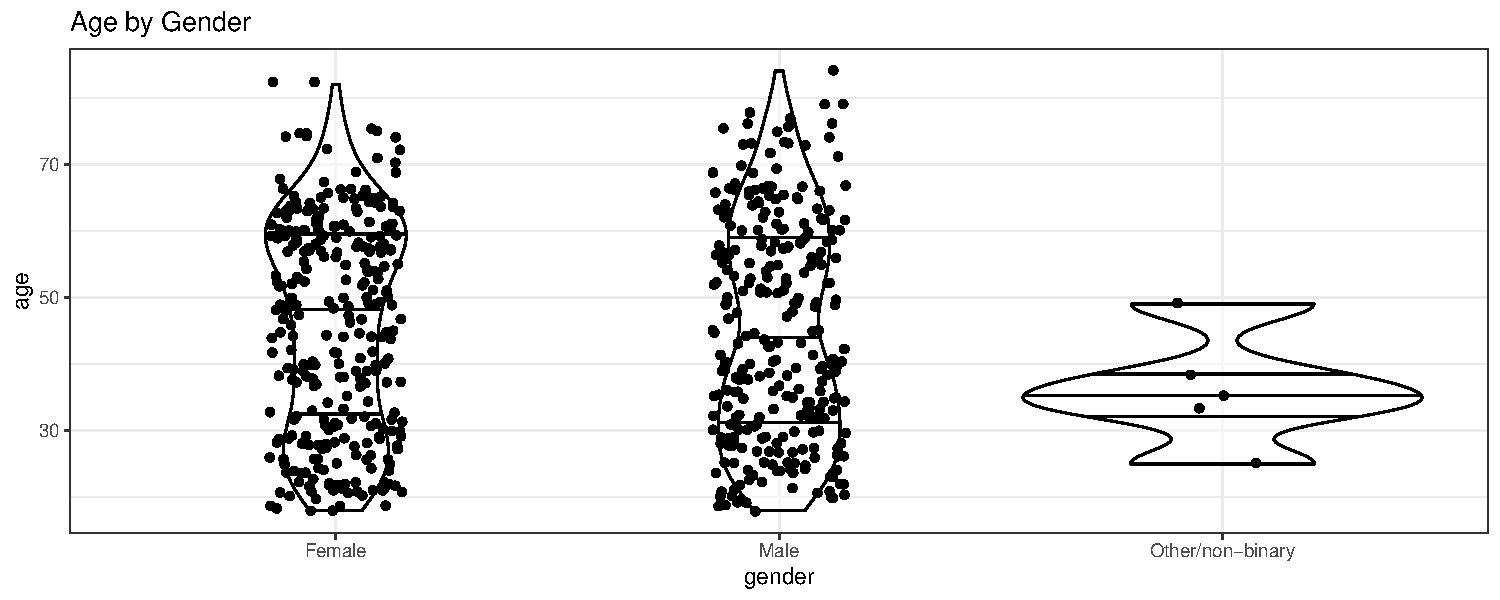
\includegraphics[width=\linewidth]{thesis_files/figure-latex/demographics-1} 

}

\caption{Demographic Information}\label{fig:demographics}
\end{figure}

Of the 636 participants with Prolific ID's who started the survey, there were 324 female participants, 307 male participants, and 5 non-binary participants.
\authorcol{These participants are a representative sample (in terms of age, sex and ethnicity, based on census data) of Prolific participants who are located in the United States.}
The median age was 45.
Age and gender are shown in Figure \ref{fig:demographics}.
An age of 0.2 was excluded due to implausibility and lack of study completion.
591 participants eligible for analysis completed the survey, and 569 participants correctly answered both attention check questions.
\authorcol{In two instances, participants reported being removed from the survey website prior to survey completion, which may have happened in other cases where the participants did not complete the survey.}
The division of correct answers on the attention check questions are shown in Table \ref{tab:attentioncheck}.
These 569 participants were considered for the following analysis.

\begin{table}

\caption{\label{tab:attentioncheck}Attention Check Information}
\centering
\begin{tabular}[t]{l|r|r}
\hline
  & Reading Correct & Reading Incorrect\\
\hline
Caliber Correct & 569 & 12\\
\hline
Caliber Incorrect & 10 & 0\\
\hline
\end{tabular}
\end{table}

\hypertarget{overview}{%
\subsection{Overview}\label{overview}}

Participants were asked a variety of questions in order to assess their thoughts and feelings on the case and the evidence presented.
Two questions related to probability: respondents were asked to provide a value for the probability that the gun was at the crime scene, and to provide a value for the probability that Richard Cole (the defendant) committed the crime.
Another question asked participants if they would convict Cole, based on the evidence.
Questions of credibility, reliability, and scientificity were assessed using a 7-point Likert scale (eg. ``Extremely unscientific'' to ``Extremely scientific'').
Understanding was ranked on a 5-point Likert scale (``I understood nothing'' to ``I understood everything'').
Participants were also asked about uniqueness of firearm toolmarks, as a simple yes/no question.
Strength of evidence was ranked on a 9-point Likert scale (``Not at all strong'' to ``Extremely strong''). The perceived frequency with which firearms examiners made mistakes was assessed on a 7-point Likert scale (``Never'' to ``Always'').

\hypertarget{probability}{%
\subsection{Probability}\label{probability}}

There is a difference in the perceived probability that Cole committed the crime as well as the perceived probability that the gun was present at the crime scene based on the examiner's decision, as shown in Figure \ref{fig:probalgorithm}.
The match condition resulted in high probabilities, while the non-match condition resulted in low probabilities, indicating that participants reacted to the examiner's testimony.
A wider range of probability values were observed for the inconclusive decision, without the high peaks that were present for conclusive decisions.
Definite conclusions of match or not a match resulted in higher peaks at more extreme values for the probability that the gun was at the crime scene, compared with the probability that Cole committed the crime.
This may indicate that some individuals are distinguishing between evidence that the weapon was used and evidence against Cole.
The inconclusive decision resulted in a more spread out distribution that is practically the same for both the probability that the gun was at the crime scene and the probability that Cole committed the crime, with participants generally selecting values below 50\%.

For both Cole and the gun, values are slightly more concentrated toward the lower end of the scale when the algorithm is absent for the non-match condition, and the inconclusive decision produced similar densities across both algorithm conditions.
In the case of the gun's involvement, values are more concentrated toward the higher end of the scale when the algorithm is present for the match condition.
There is no real difference between match distributions for the probability that Cole committed the crime.
The vertical lines indicate the match score presented by the algorithm (0.034 or 3.4\% for the non-match condition, 0.34 or 34\% for the inconclusive condition, and 0.989 or 98.9\% for the match condition).
These are displayed in order to visually assess whether the subjects are anchoring to the given match score when assessing the probability of the gun being present at the crime scene.
Because the match score is on a scale of 0 to 1, this value could be misinterpreted as a probability for the gun being used in the crime.
It does not appear that the participants are anchoring to this value, however, as the distributions do not correspond more to the line when the algorithm is present.

\begin{figure}

{\centering 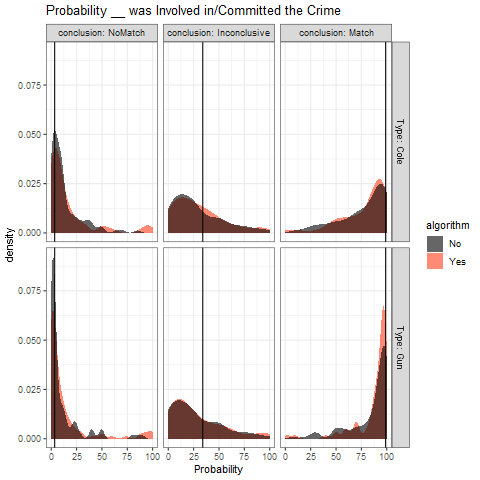
\includegraphics[width=\linewidth]{images/probalgorithm} 

}

\caption{Probability the gun was used in the crime, or that Cole committed the crime. Black lines indicate bullet match scores for the algorithm.}\label{fig:probalgorithm}
\end{figure}

\hypertarget{probability-and-guilt}{%
\subsubsection{Probability and Guilt}\label{probability-and-guilt}}

After reading the testimony, the participants were given the following question:
``The State has the burden of proving beyond a reasonable doubt that the defendant is the person who committed the alleged crime.
If you are not convinced beyond a reasonable doubt that the defendant is the person who committed the alleged crime, you must find the defendant not guilty.
Would you convict this defendant, based on the evidence that you have heard?''
10 out of 196 individuals in the non-match category, 13 out of 191 individuals in the inconclusive category, and 112 out of 182 individuals in the match category chose to convict, despite the bullet matching being the only evidence against Cole in the crime.
As \ref{fig:probguilt} illustrates, across all categories individuals who chose to convict generally assigned a higher probability to Cole committing the crime than those who did not choose to convict.
The same general trend of higher probability values for those who chose to convict and lower probability values for those who chose not to convict is also seen for non-match and inconclusive conditions when discussing the probability that the gun was used in the crime.
However, in the case of the match condition, those who did not convict gave a generally higher probability that the gun was used in the crime than the probability that Cole committed the crime, resulting in comparable values (albeit with more variability) to those who chose to convict.

\begin{figure}

{\centering 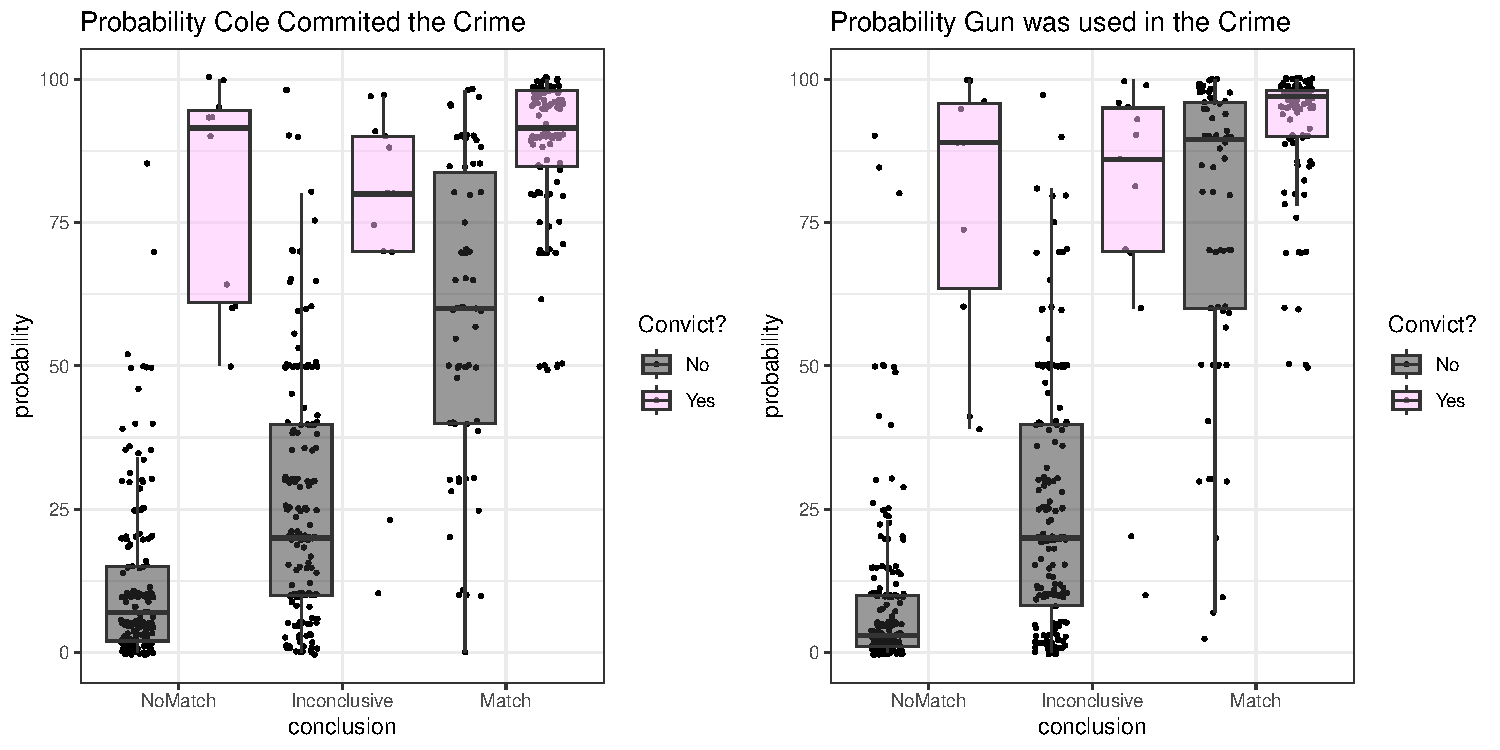
\includegraphics[width=\linewidth]{thesis_files/figure-latex/probguilt-1} 

}

\caption{Probabilities based on whether the participants thought the defendant was guilty}\label{fig:probguilt}
\end{figure}

\hypertarget{credibility}{%
\subsection{Credibility}\label{credibility}}

Through all conditions, the level of credibility remained approximately the same for both the firearms examiner and the algorithm expert.
As Figure \ref{fig:cred} demonstrates, ``Extremely credible'' was by far the most selected category for the firearms examiner, with some people selecting ``Moderately credible'', while the other categories quickly drop off in responses.
This trend was also reflected in the data for the algorithm expert, and can be seen in most histograms resulting from this study (leading to a question of scale compression).
The lack of difference based on examiner decision, image, or algorithm (in the case of the firearms examiner) provides a hopeful indication that the credibility of expert witnesses is not necessarily swayed by the facts of the case or the presence of images, when their written testimony remains the same.

\begin{figure}

{\centering 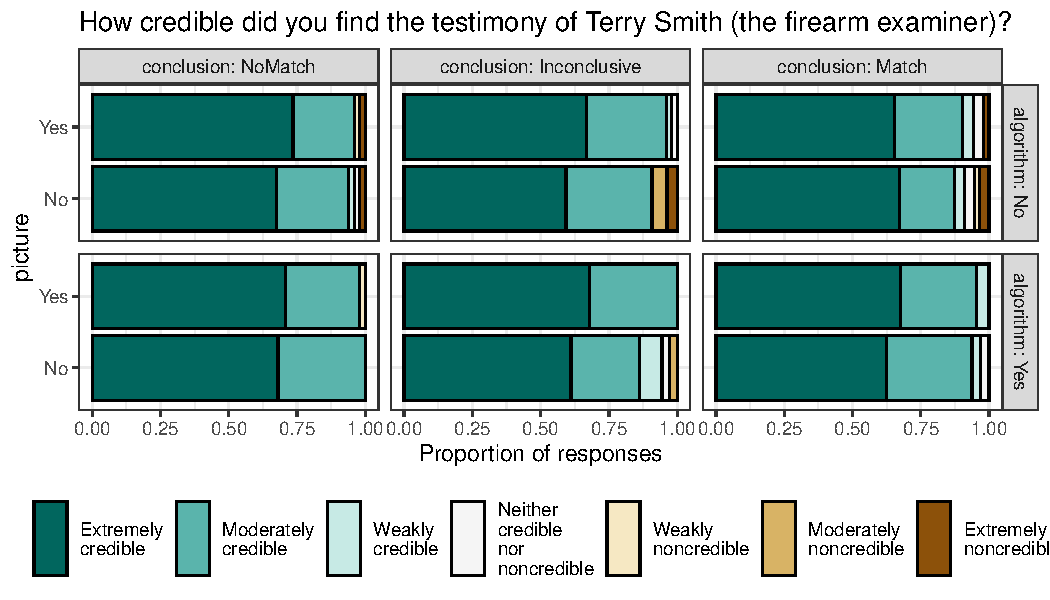
\includegraphics[width=\linewidth]{thesis_files/figure-latex/cred-1} 

}

\caption{Histogram of Firearms Examiner Credibility}\label{fig:cred}
\end{figure}

\hypertarget{reliability}{%
\subsection{Reliability}\label{reliability}}

In terms of reliability, participants appeared to find the case evidence less reliable when an inconclusive decision was given than they did when a conclusive decision was reached, as shown in Figure \ref{fig:caserel}.
Note that this question was only answered by participants who received the algorithm condition and is meant to encompass both the examiner's comparison and the algorithm comparison.
As with the credibility condition, the majority of individuals selected the two highest conditions, ``Moderately reliable'' and ``Extremely reliable'', across all categories of conclusions.
In the case of an inconclusive decision, the highest proportion of participants selected ``Moderately reliable'', while for the conclusive decisions, the highest proportion of participants selected ``Extremely reliable''.

\begin{figure}

{\centering 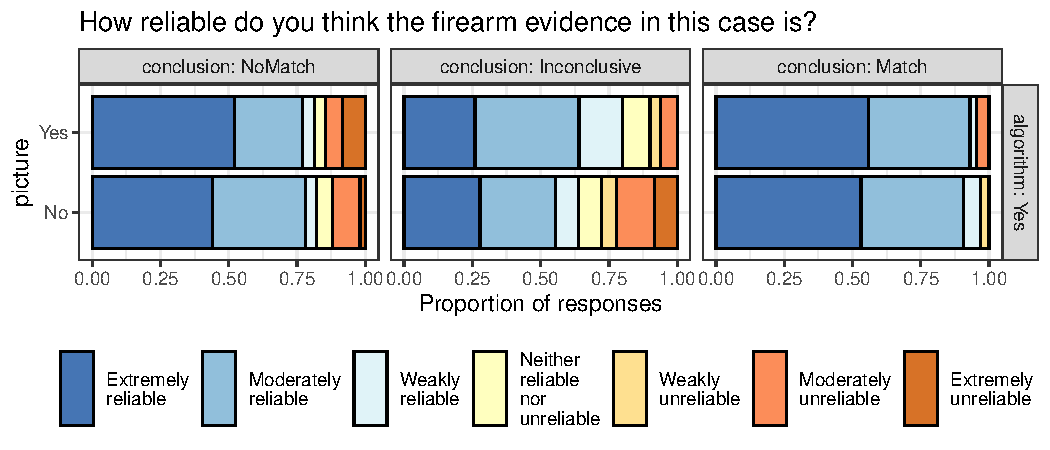
\includegraphics[width=\linewidth]{thesis_files/figure-latex/caserel-1} 

}

\caption{Histogram of overall case reliability}\label{fig:caserel}
\end{figure}

Individuals were also asked to rate the general reliability of firearms evidence as a field (Figure \ref{fig:genrel}).
As with case reliability, those who received an inconclusive condition were more likely to select ``Moderately reliable'' than they were to select ``Extremely reliable''.
This trend is also shown in the non-match condition when the algorithm is present.
However, it is not reflected in the match condition.
When the algorithm is absent, both the match and the non-match conditions appear to produce approximately equal proportions for the two highest categories of reliability.
As with previous responses, all other categories are sparsely populated.

\begin{figure}

{\centering 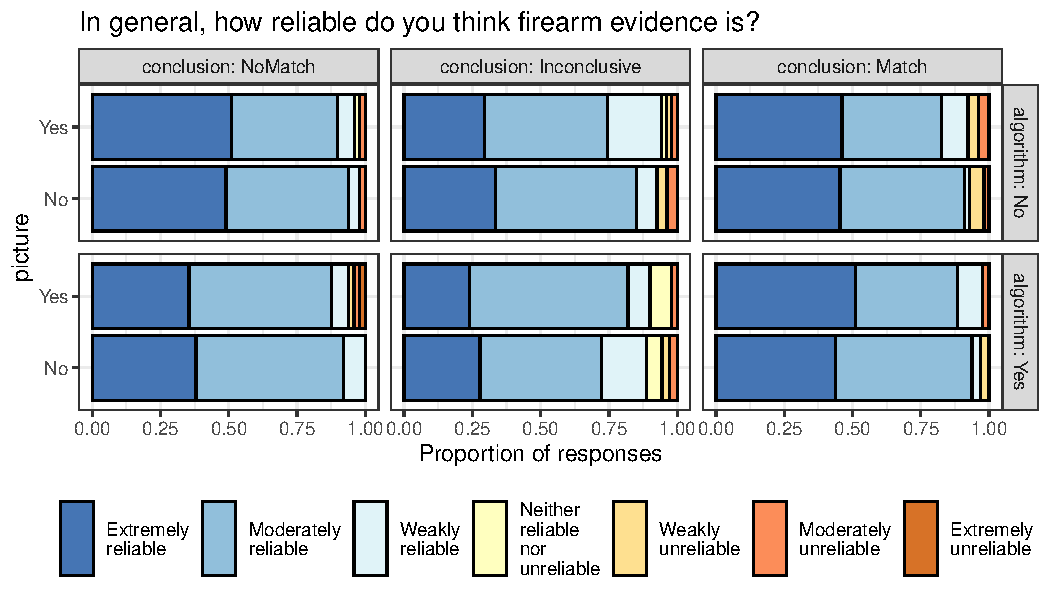
\includegraphics[width=\linewidth]{thesis_files/figure-latex/genrel-1} 

}

\caption{Histogram of perceived firearm reliability as a field}\label{fig:genrel}
\end{figure}

In all conditions, participants were asked to rate the reliability of the examiner's subjective opinion of the firearm evidence (Figure \ref{fig:examrel}).
Participants from both the algorithm and non-algorithm groups gave similar reliability ratings in the non-match condition: most chose ``Moderately reliable'' or ``Extremely reliable'', with more choosing ``Extremely reliable''.
For inconclusive and match conditions, there is a difference in proportions of which category is selected based on the presence or the absence of the algorithm.
When the algorithm is absent, the trend is fairly similar to that in the non-match condition: between the two highest categories, the majority chose ``Extremely reliable''.
However, in the case that the algorithm was present, this trend was flipped: more participants chose ``Moderately reliable'' over ``Extremely reliable''.

\begin{figure}

{\centering 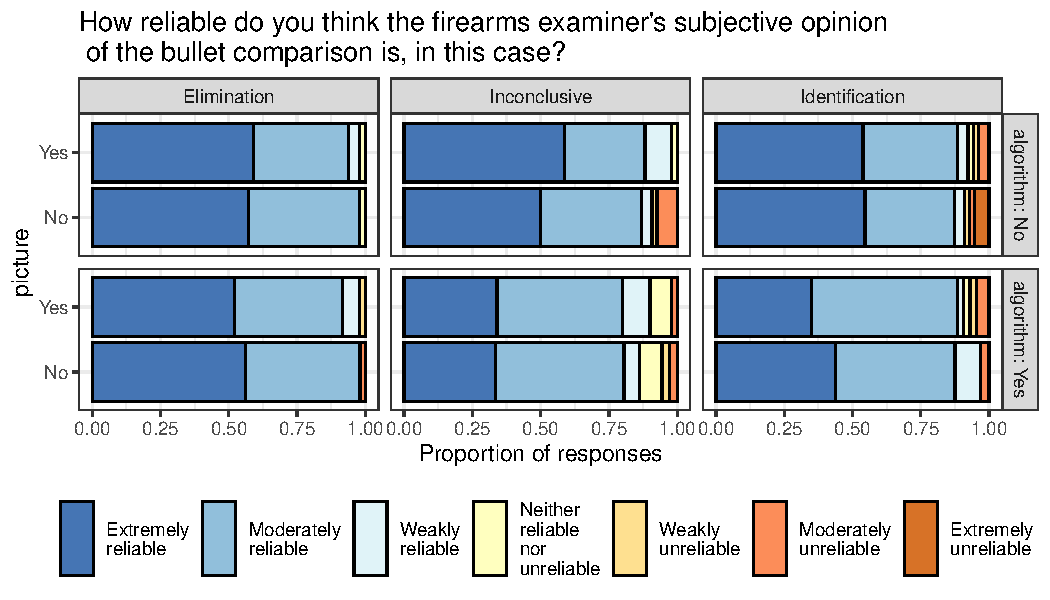
\includegraphics[width=\linewidth]{thesis_files/figure-latex/examrel-1} 

}

\caption{Histogram of perceived firearm exam reliability}\label{fig:examrel}
\end{figure}

Individuals who received the algorithm were also asked to rate algorithm reliability, responses are shown in Figure \ref{fig:algrel}.
The responses were in many ways similar to those given in the case of general reliability: those who received an inconclusive decision were more likely to give a lower reliability rating, and the two highest categories were by far the most selected.
Both also demonstrated a higher selection of ``Weakly reliable'' when individuals were presented with an inconclusive decision.

\begin{figure}

{\centering 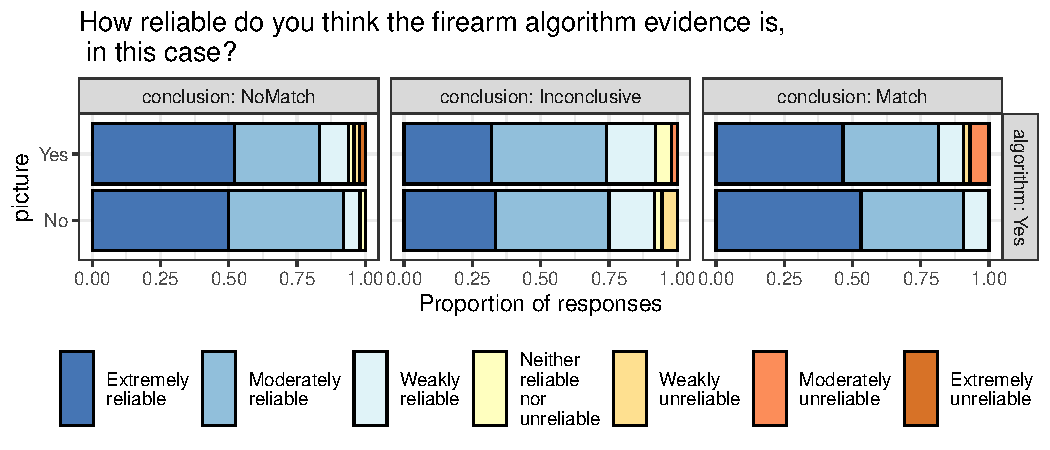
\includegraphics[width=\linewidth]{thesis_files/figure-latex/algrel-1} 

}

\caption{Histogram of perceived algorithm reliability}\label{fig:algrel}
\end{figure}

In most cases, individuals gave lower reliability ratings when an inconclusive decision was reached.
They also tended to select the two highest reliability categories, ``Moderately reliable'' and ``Extremely reliable'', regardless of other conditions.
The presence or absence of images did not have a noticeable effect on reliability ratings.
The presence of the algorithm is related to a slight reduction in reliability ratings for the firearms examiner's personal bullet comparison, in the case of an inconclusive or match decision.

\hypertarget{scientificity}{%
\subsection{Scientificity}\label{scientificity}}

Participants were also asked about how scientific they felt the process was, in a similar four-question format to reliability.
These results bore some similarity in responses to reliability across questions.
As previously stated, images did not appear to have a large effect and the two highest categories were by far the most selected.
When asked about their rating of how scientific the evidence was in the case overall, those receiving the inconclusive condition were less likely to select ``Extremely scientific'' compared to their counterparts given conclusive conditions.

In terms of firearms evidence as a field, results are shown in Figure \ref{fig:gensci}.
Here, as before, those who received the inconclusive decision were more likely to select ``Moderately scientific'' over ``Extremely scientific'' for both cases of the algorithm.
A higher proportion of individuals selected ``Extremely scientific'' for conclusive decisions when the algorithm was present compared to when the algorithm was absent.

\begin{figure}

{\centering 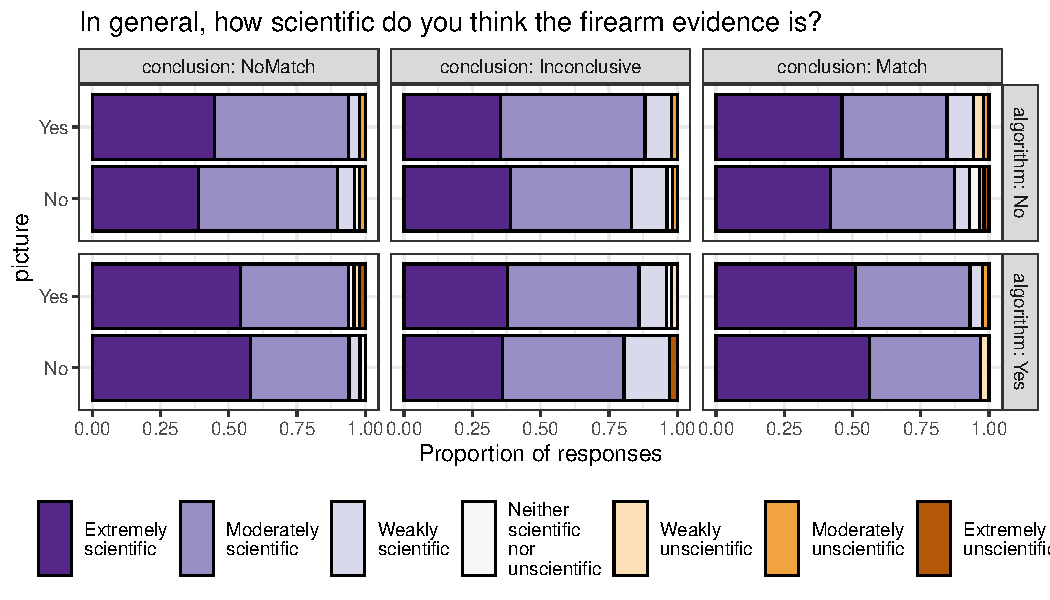
\includegraphics[width=\linewidth]{thesis_files/figure-latex/gensci-1} 

}

\caption{Histogram of perceived firearm scientificity as a field}\label{fig:gensci}
\end{figure}

Regarding how scientific individuals found the examiner's comparison, the algorithm only seemed to have an effect when individuals were presented with an inconclusive decision (\ref{fig:examsci}).
When the algorithm was not present, people were more likely to select ``Extremely scientific'', resulting in a proportion on par with conclusive results.
When the algorithm was present, however, ``Moderately scientific'' became the most popular choice for those who received an inconclusive decision, which reflects the general trend of the majority of participants selecting the second highest category for inconclusive results.
Results for conclusive categories are fairly similar across algorithm conditions, with a close split between ``Moderately scientific'' and ``Extremely scientific''.

\begin{figure}

{\centering 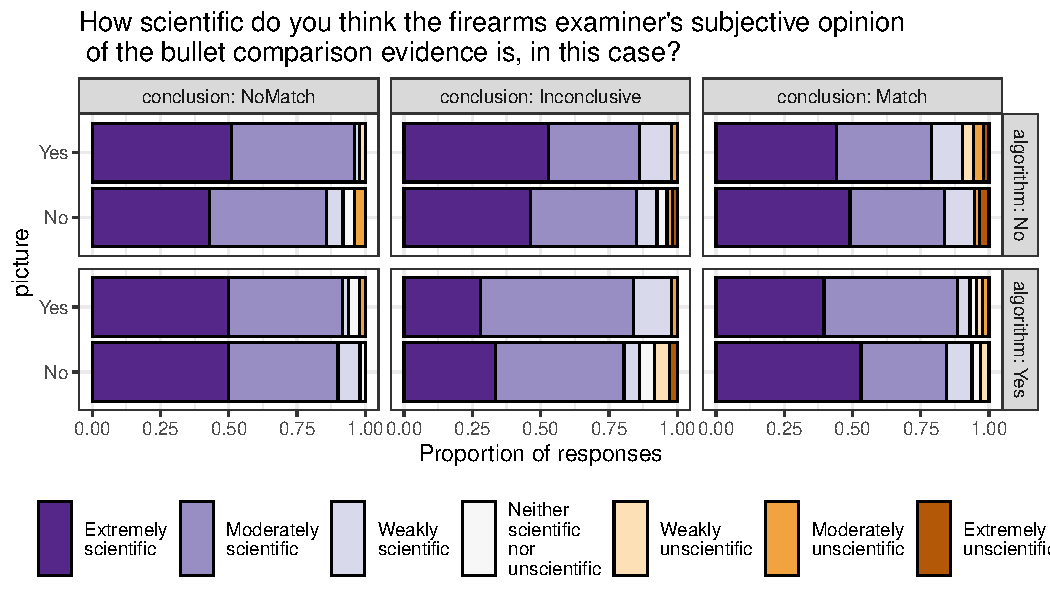
\includegraphics[width=\linewidth]{thesis_files/figure-latex/examsci-1} 

}

\caption{Histogram of perceived scientificity of the bullet comparison of the firearm examiner}\label{fig:examsci}
\end{figure}

Participants gave the algorithm a high rating in scientificity across all categories of conclusions, as shown in Figure \ref{fig:algsci}.
Here, all decisions had the highest proportion of respondents select ``Extremely scientific''.
The proportion selecting ``Moderately scientific'' was noticeably lower than the proportion selecting ``Extremely scientific''.
The use of demonstrative evidence did not have a visible effect.

\begin{figure}

{\centering 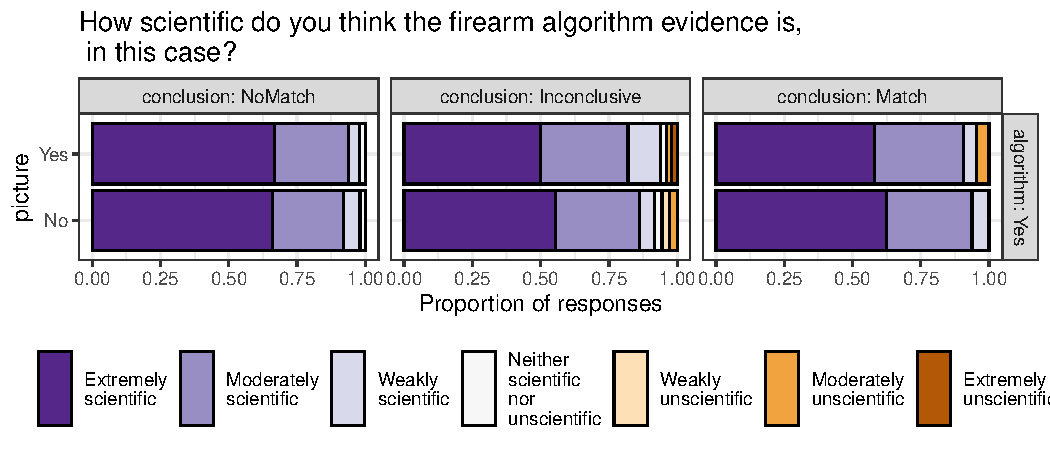
\includegraphics[width=\linewidth]{thesis_files/figure-latex/algsci-1} 

}

\caption{Histogram of perceived algorithm scientificity in this case}\label{fig:algsci}
\end{figure}

In summary, the algorithm is related an an increase of perceived scientificity for the field of firearm evidence as a whole when individuals were presented with a conclusive decision, and ``Extremely scientific'' was the most selected category when evaluating the scientificity of the algorithm evidence regardless of conclusion.
As for how individuals rated the scientificity of the algorithm expert's comparison, the algorithm only appeared to influence results for those who received the inconclusive condition.
Individuals who received the algorithm were more likely to select ``Moderately scientific'', while those who did not receive the algorithm were more likeley to select ``Extremely scientific''.

\hypertarget{understanding}{%
\subsection{Understanding}\label{understanding}}

Individuals were asked to rate their understanding of both the algorithm and the examiner's personal bullet comparison on a 5-point Likert scale. Most responses ranged from 3 (``I understood about half of the method'') to 5 (``I understood everything''), leading to less scale compression than was seen in scales relating to credibility, reliability, and scientificity.

For the firearms examiner's personal comparison, few individuals selected that they understood less than half the method (Figure \ref{fig:expunder}).
Those who did not receive the algorithm were more likely to select ``I understood everything'' compared to those who did receive the algorithm, across all conclusions.
There was not a discernible difference in responses based on the presence or absence of images.

\begin{figure}

{\centering 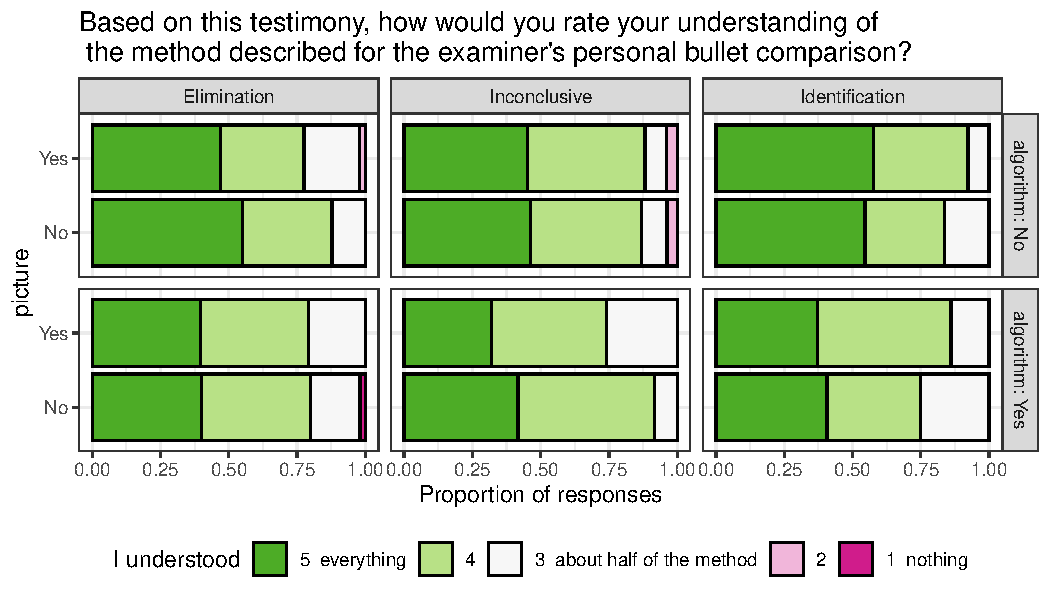
\includegraphics[width=\linewidth]{thesis_files/figure-latex/expunder-1} 

}

\caption{Histogram of understanding for the explanation of the firearms examiner}\label{fig:expunder}
\end{figure}

The results for the particpants' understanding of the algorithm description differs based on the presence or absence of images (Figure \ref{fig:algunder}).
When images are absent, participants selected values from ``I understood about half the method'' to ``I understood everything'' with a fairly uniform frequency, with a few participants selecting values in the lower categories.
When images were present, however, category selection appeared to relate to conclusion.
Those receiving the match condition were more likely to select 4 than other categories, meaning that they felt they understood more than half of the method but didn't understand everything.
Those receiving the non-match condition were more likely to select that they understood half of the method compared to other categories.
Those with an inconclusive condition had responses fairly evenly distributed across the top three categories, similar to when images were absent.
As in the case without images, few individuals indicated that they understood less than half of the method.
It is unclear what may have caused these differences in ratings of understanding.

\begin{figure}

{\centering 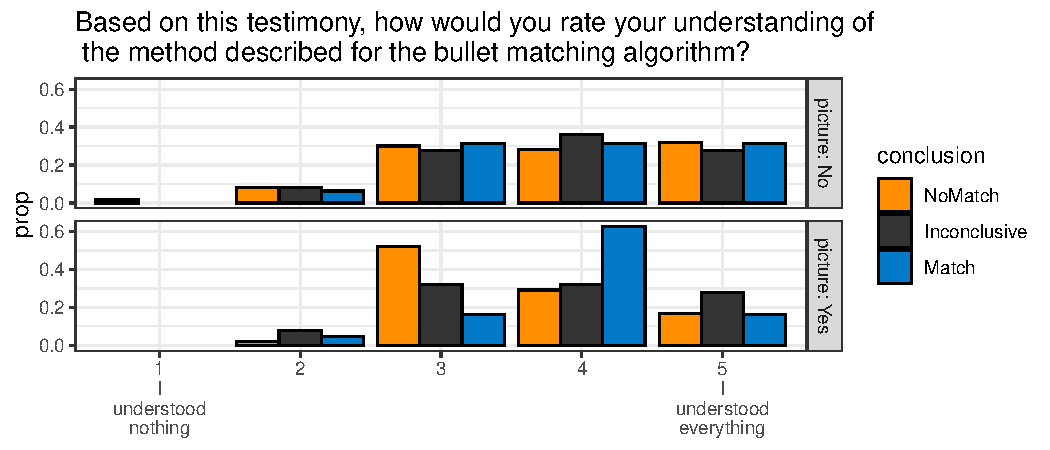
\includegraphics[width=\linewidth]{thesis_files/figure-latex/algunder-1} 

}

\caption{Histogram of understanding for the algorithm explanation}\label{fig:algunder}
\end{figure}

\authorcol{To investigate this potential relationship further, Table} \ref{tab:undertb}
\authorcol{was created. Because the counts are so small for the individual cells, the resemblence to a relationship based on conclusion is possibly due to random variation.}

\begin{table}

\caption{\label{tab:undertb}Understanding Frequency}
\centering
\begin{tabular}[t]{>{\raggedright\arraybackslash}p{10em}|r|r|r}
\hline
  & NoMatch & Inconclusive & Match\\
\hline
1
I
understood
nothing & 0 & 0 & 0\\
\hline
2.0 & 1 & 4 & 2\\
\hline
3
I
understood
about
half
of
the
method & 25 & 16 & 7\\
\hline
4.0 & 14 & 16 & 27\\
\hline
5
I
understood
everything & 8 & 14 & 7\\
\hline
\end{tabular}
\end{table}

\hypertarget{uniqueness}{%
\subsection{Uniqueness}\label{uniqueness}}

Individuals were asked whether or not they thought that guns left unique markings on discharged bullets and casings after reviewing the testimony.
Of the 569 responses, only 16 individuals indicated that they did not think guns left unique markings.
These respondents were split across conditions.
Thus, respondents in this study overwhelmingly believe in the uniqueness of markings on discharged bullets.

\hypertarget{strength}{%
\subsection{Strength}\label{strength}}

\begin{figure}

{\centering 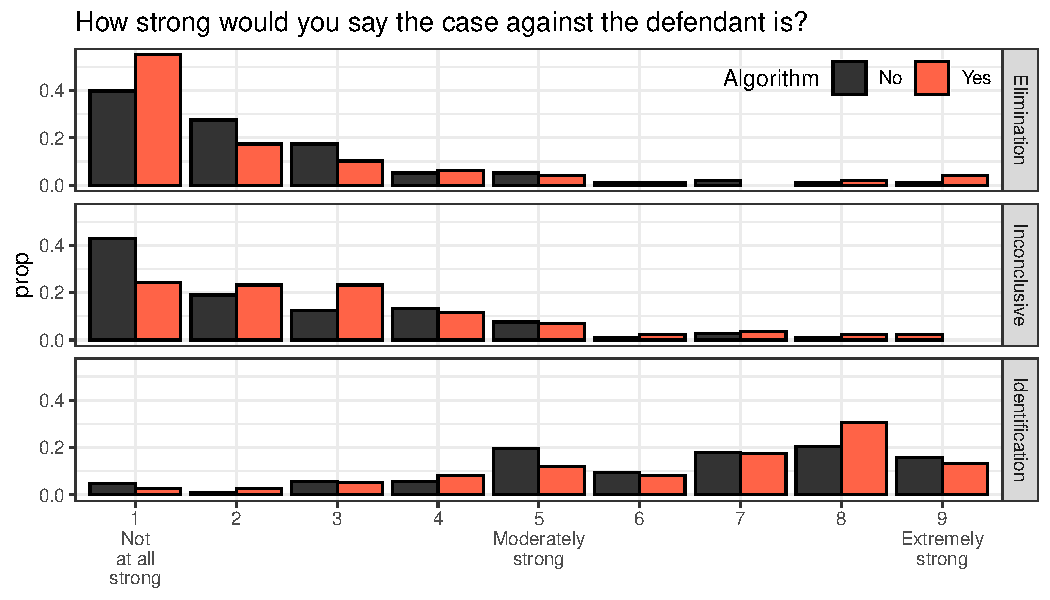
\includegraphics[width=\linewidth]{thesis_files/figure-latex/strength-1} 

}

\caption{Histogram of perceived strength of evidence against the defendant}\label{fig:strength}
\end{figure}

Individuals were also asked to rate the strength of evidence, both against Richard Cole and against the gun.

When asked about the case against the defendant, shown in Figure \ref{fig:strength}, there was a small difference in terms of the algorithm.
When the examiner reached a non-match conclusion, individuals who also received the algorithm were more likely to select the lowest category (``not at all strong'') compared to those who did not receive the algorithm.
Alternatively, in the case of an inconclusive decision, individuals who did not receive the algorithm were more likely to select ``not at all strong'' compared to those who did receive the algorithm.
For the match condition, responses were more widely distributed.

\begin{figure}

{\centering 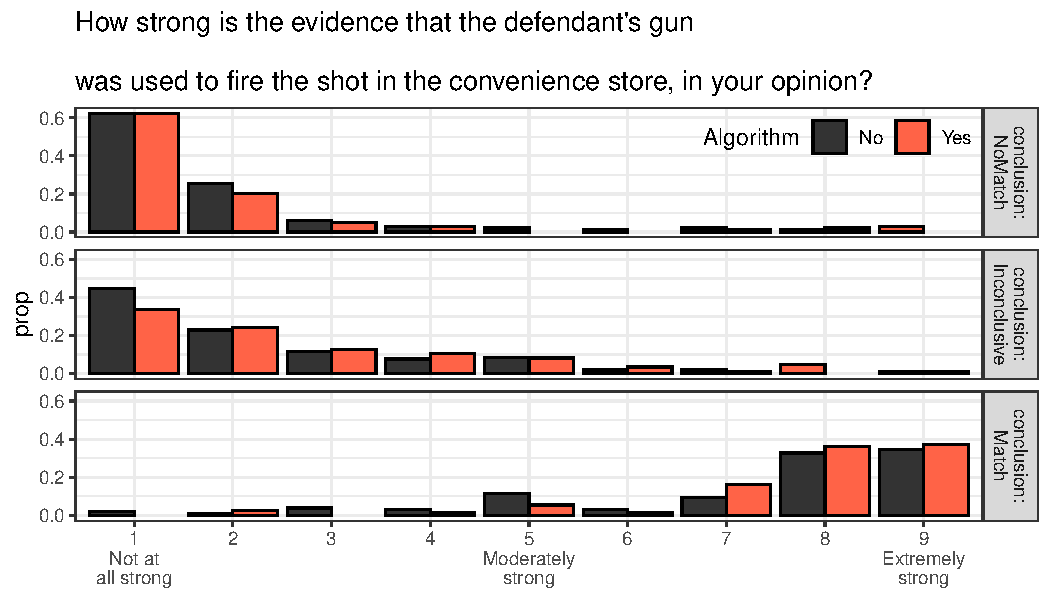
\includegraphics[width=\linewidth]{thesis_files/figure-latex/gunstrength-1} 

}

\caption{Histogram of perceived strength of evidence against the gun}\label{fig:gunstrength}
\end{figure}

When asked about the strength of evidence against the defendant's gun, there was no real difference between those who received the algorithm and those who did not (\ref{fig:gunstrength}).
The match condition resulted in a more concentrated distribution at higher strength values than were seen for the strength of evidence against Cole.

\begin{figure}

{\centering 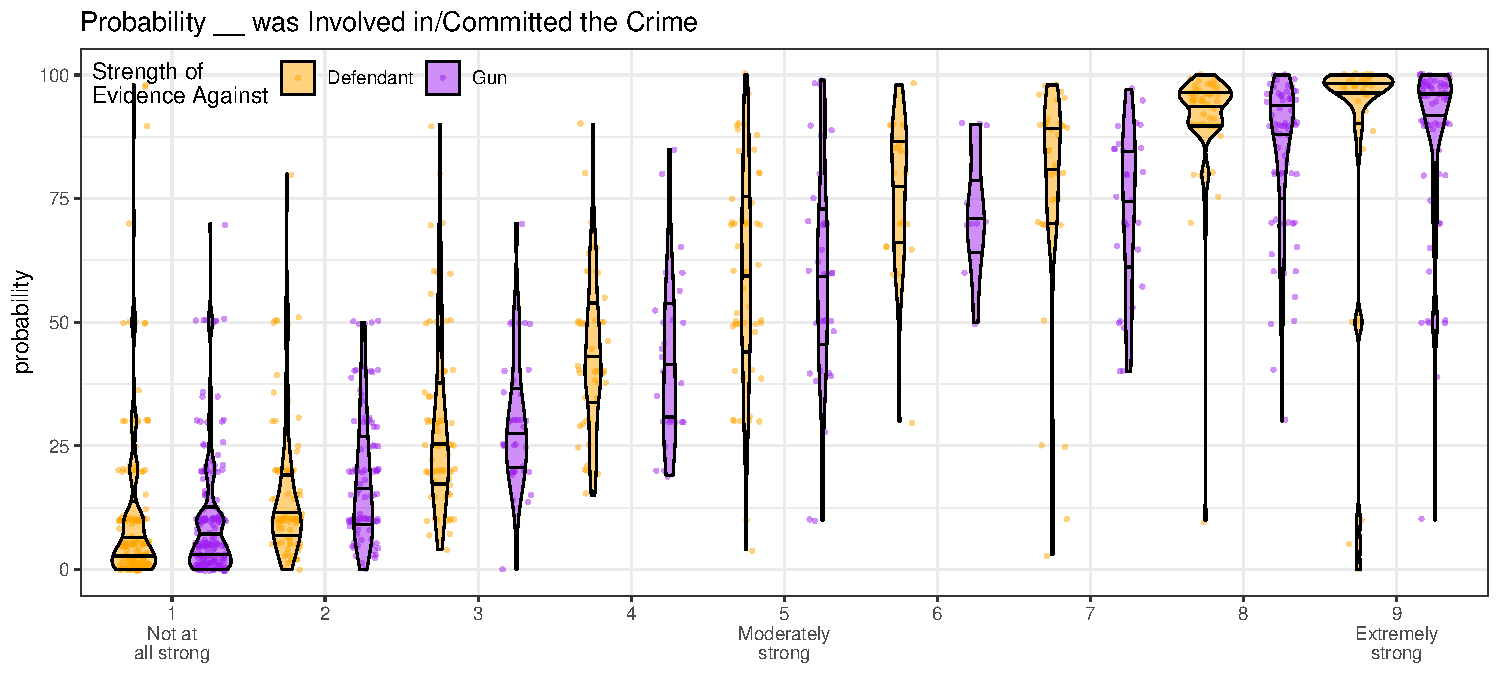
\includegraphics[width=\linewidth]{thesis_files/figure-latex/probstrength-1} 

}

\caption{Probabilities based on perceived strength of evidence.}\label{fig:probstrength}
\end{figure}

In comparing how individuals scored strength of evidence and the probability that they assigned to Cole committing the crime and the gun being present at the crime scene, the results were largely consistent (\ref{fig:probstrength}).
In general, the probability assigned increases as the assigned strength of evidence increases, which is to be expected.

\hypertarget{mistakes}{%
\subsection{Mistakes}\label{mistakes}}

Individuals were asked how often firearms examiners make mistakes when determining whether bullets were fired through the same gun, with a scale from ``Never'' to ``Usually''.
``Rarely'' was by far the most selected category, as shown in Figure \ref{fig:mistakes}.
There does not appear to be a strong relationship between how often individuals felt firearms examiners made mistakes and factors such as conclusion, images, or the algorithm.

\begin{figure}

{\centering 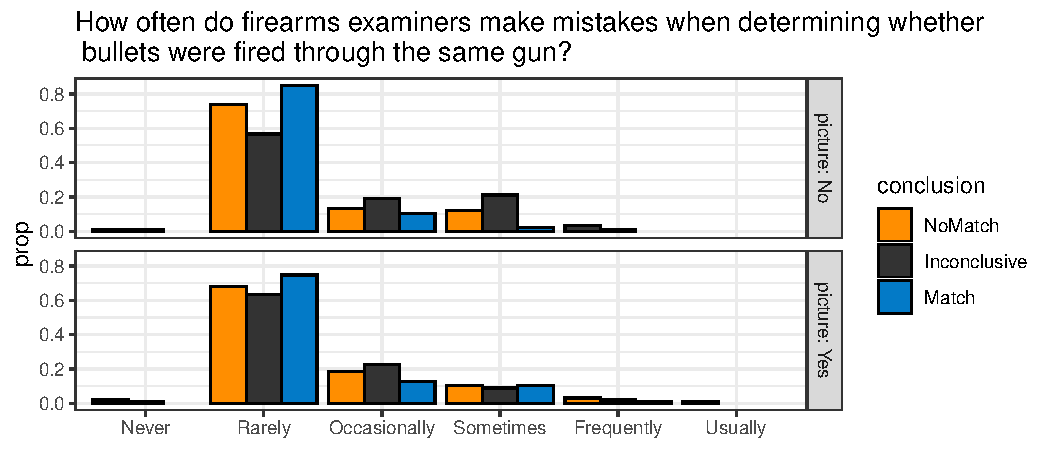
\includegraphics[width=\linewidth]{thesis_files/figure-latex/mistakes-1} 

}

\caption{Histogram of perceived frequency of mistakes made by firearms examiners}\label{fig:mistakes}
\end{figure}

\hypertarget{comparing-algorithm-values-to-examiner-values}{%
\subsection{Comparing Algorithm Values to Examiner Values}\label{comparing-algorithm-values-to-examiner-values}}

Participants who received the algorithm condition were asked to evaluate their feelings on the reliability, credibility, scientificity, and their understanding of both the algorithm method as well as the traditional bullet analysis method, as discussed in previous sections.
Results for both methods were compared on an individual level as well as on a group level.
The group level results are represented in histograms, while the individual level results are represented in parallel coordinates plots.
Note that these results only reflect the feelings of individuals who received the algorithm condition.

\hypertarget{group-level-results}{%
\subsubsection{Group Level Results}\label{group-level-results}}

\begin{figure}

{\centering 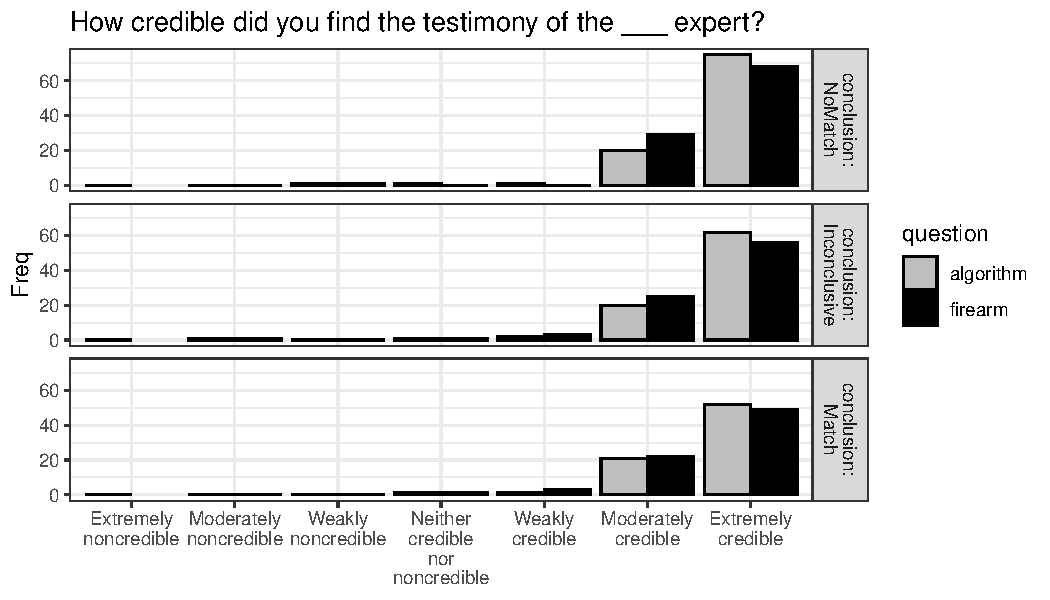
\includegraphics[width=\linewidth]{thesis_files/figure-latex/histcred-1} 

}

\caption{Histogram of perceived credibility of experts}\label{fig:histcred}
\end{figure}

In terms of credibility, as shown in Figure \ref{fig:histcred}, the algorithm and the expert scored fairly similarly, with the algorithm expert resulting in slightly more individuals selecting ``Extremely credible'' than the firearms expert.
As mentioned before, most participants limited their selection to the two highest categories - ``Moderately credible'' and ``Extremely credible''.

\begin{figure}

{\centering 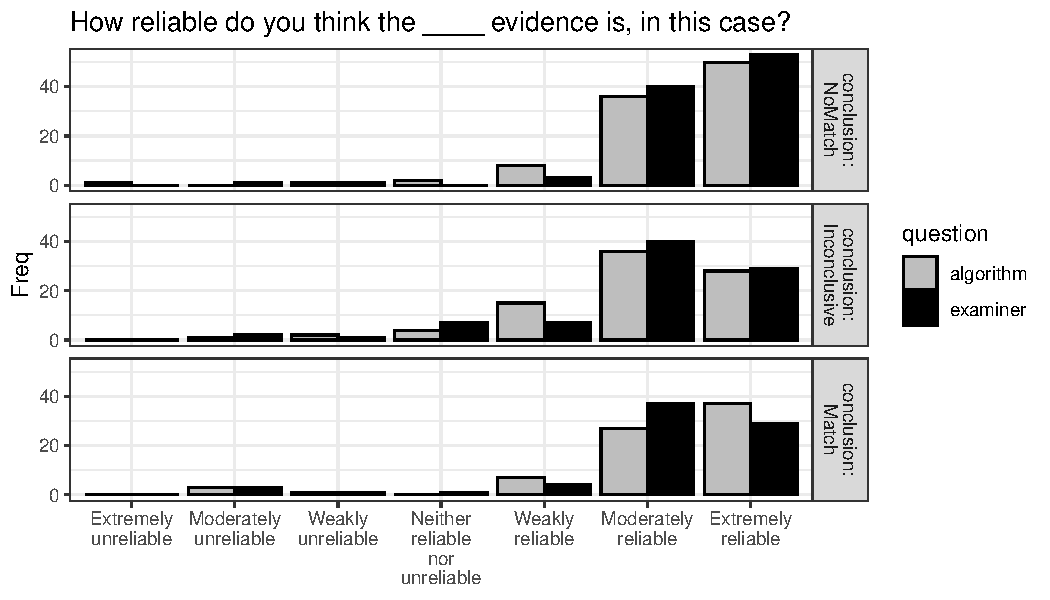
\includegraphics[width=\linewidth]{thesis_files/figure-latex/histrel-1} 

}

\caption{Histogram of perceived reliability of evidence}\label{fig:histrel}
\end{figure}

For reliability, shown in Figure \ref{fig:histrel}, a similar number of individuals selected ``Extremely reliable'' for both the algorithm evidence and the examiner's comparison, with a larger proportion of individuals selecting ``Extremely reliable'' in the match condition when the algorithm is present.
There appears to be, however, a difference in the categories of ``Moderately reliable'' and ``Weakly reliable''.
Individuals were more likely to select that the algorithm was ``Weakly reliable'', while they were less likely to select that the algorithm was ``Moderately reliable'', compared to the examiner.

\begin{figure}

{\centering 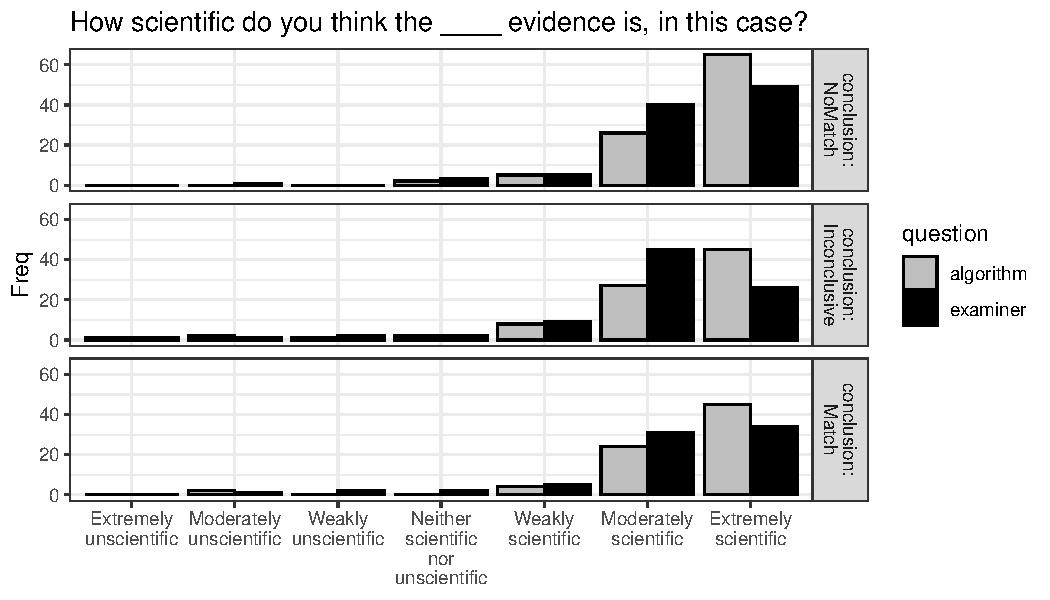
\includegraphics[width=\linewidth]{thesis_files/figure-latex/histsci-1} 

}

\caption{Histogram of perceived scientificity of evidence}\label{fig:histsci}
\end{figure}

Individuals generally saw the algorithm as more scientific than the expert, as shown in Figure \ref{fig:histsci}.
They were more likely to select ``Extremely scientific'' in the case of the algorithm when compared to the expert.
Accordingly, they were less likely to select ``Moderately scientific'' in the case of the algorithm when compared to the examiner.
No real difference can be seen in the lower values on the scale, due to few individuals selecting these categories.

\begin{figure}

{\centering 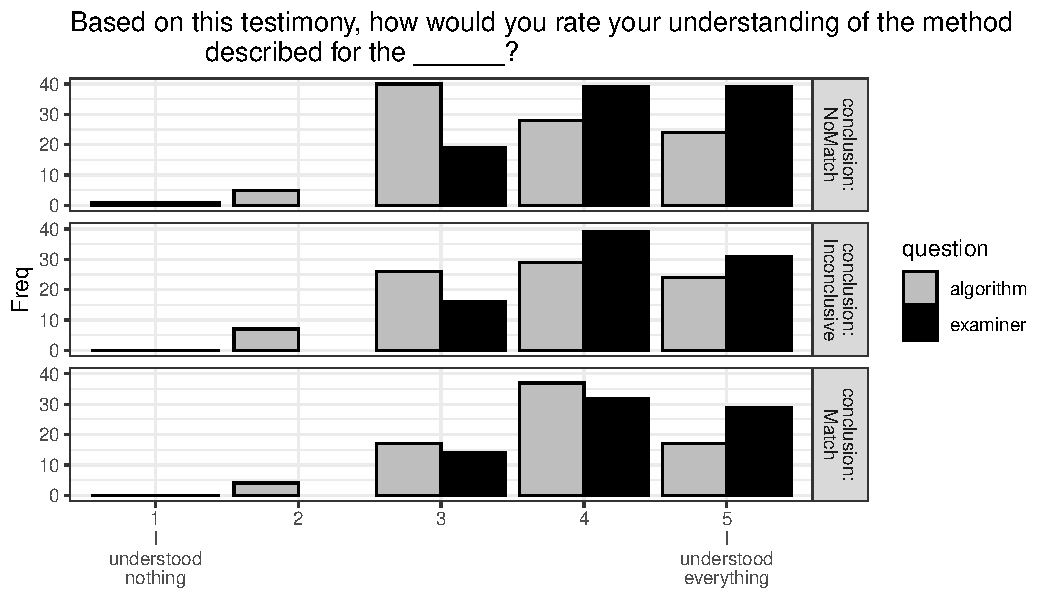
\includegraphics[width=\linewidth]{thesis_files/figure-latex/histunder-1} 

}

\caption{Histogram of participants' understanding}\label{fig:histunder}
\end{figure}

Individuals rated their understanding of the examiner's bullet comparison higher than their understanding of the algorithm method, generally speaking (\ref{fig:histunder}).
Participants were more likely to select a 4 or 5 with regards to their understanding of the examiner's comparison, while they were more likely to select a 3 or 4 with regards to their understanding of the algorithm method.

\hypertarget{individual-level-results}{%
\subsubsection{Individual Level Results}\label{individual-level-results}}

\begin{figure}

{\centering 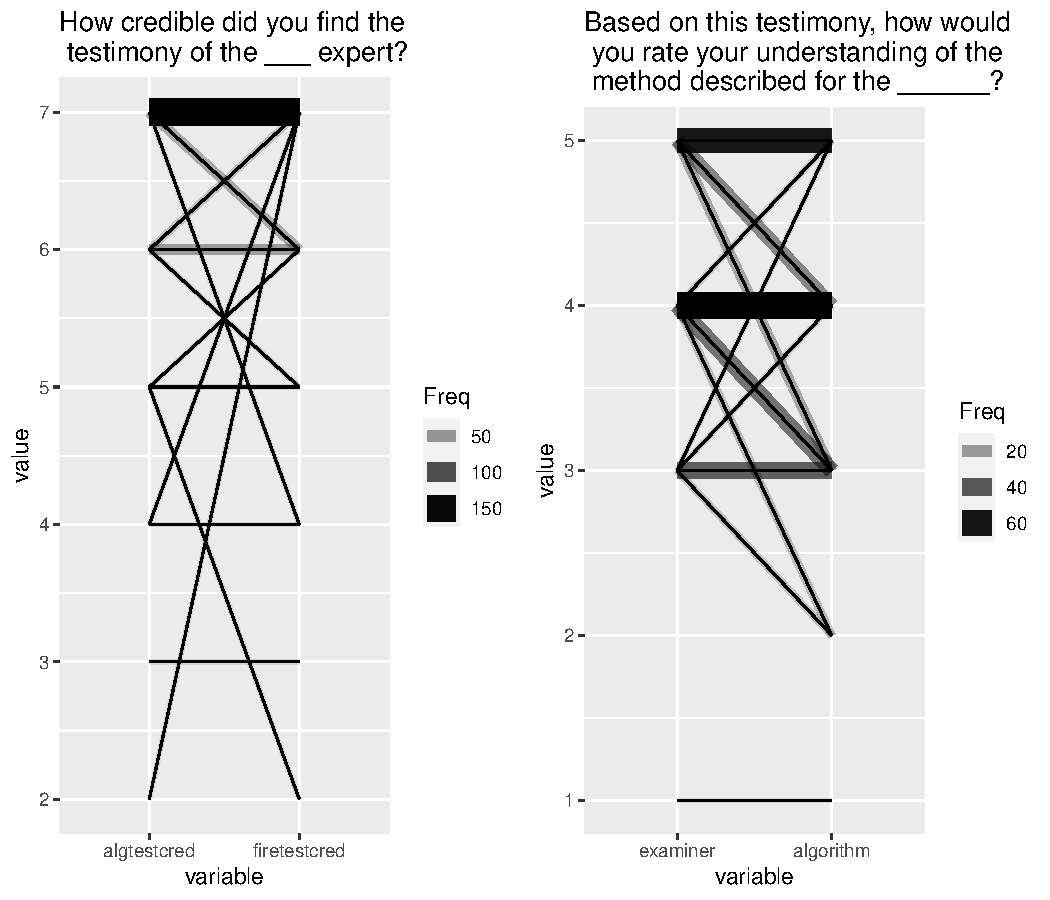
\includegraphics[width=\linewidth]{thesis_files/figure-latex/coordcred-1} 

}

\caption{Plots of understanding and perceived expert credibility}\label{fig:coordcred}
\end{figure}

Figure \ref{fig:coordcred} depicts parallel coordinate plots for participants' ratings of the credibility of the experts, as well as their understanding of the methods described in the testimony.
Higher values indicate higher scores in understanding and credibility. These plots map the frequency that individuals selected the shown combination of values for credibility or understanding.
In the case of credibility, we can see that most individuals selected the highest category of credibility for both the algorithm and the firearms expert.
In the case of understanding, individuals tended to select the two highest categories the most.
It can also be seen that there is a trend of individuals selecting a category lower for the algorithm compared to what they selected for the examiner by the thicker downward line between categories 4 and 5, as well as between categories 4 and 3.
This corresponds to Figure \ref{fig:histunder} in that individuals tend to give higher understanding ratings to the examiner's bullet comparison method than they did for the algorithm.

\begin{figure}

{\centering 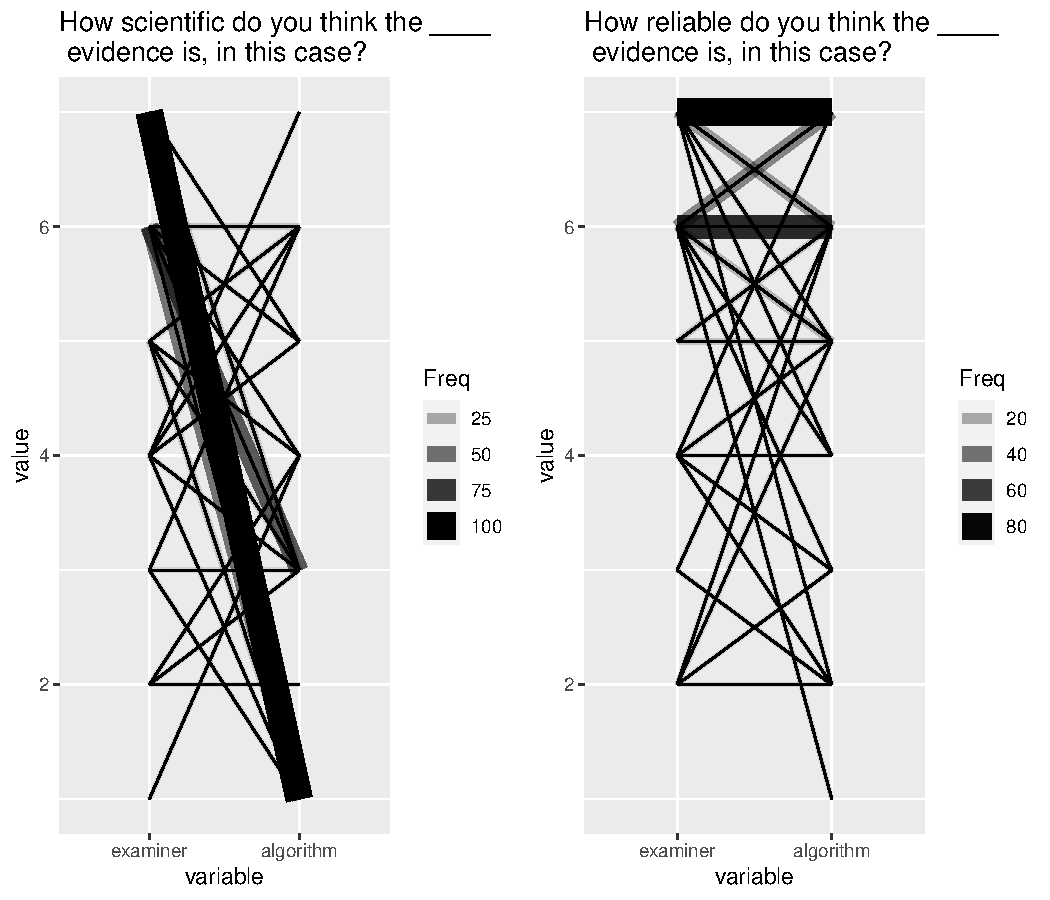
\includegraphics[width=\linewidth]{thesis_files/figure-latex/coordscirel-1} 

}

\caption{Plots of perceived scientificity and reliability of methods}\label{fig:coordscirel}
\end{figure}

Figure \ref{fig:coordscirel} demonstrates the trends for selection for how scientific and reliable individuals felt the evidence was.
In terms of how scientific individuals felt the evidence was, it appears that most participants selected the highest category for both the algorithm and the examiner.
Some participants selected the second highest category for the examiner, and the highest category for the algorithm.
Others selected the second highest category in both cases.
In terms of reliability, participants tended to choose one of the two highest categories for both the algorithm and the examiner.
Some participants switched between the two highest categories for the algorithm or the examiner, in similar numbers.

\begin{figure}
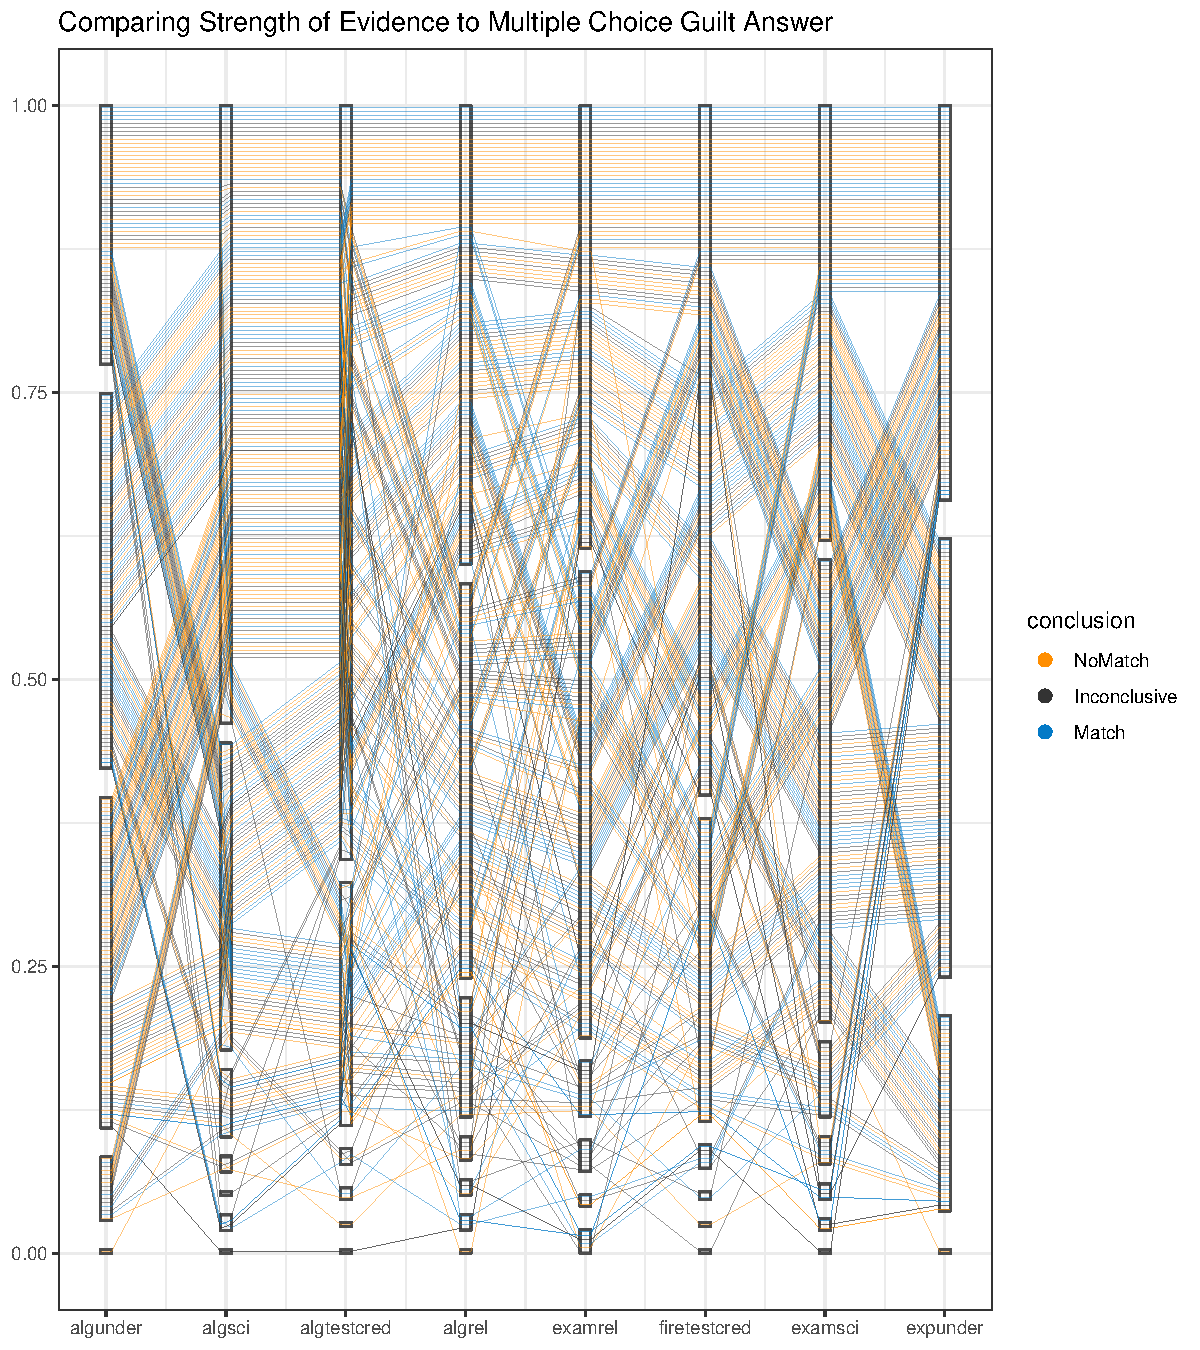
\includegraphics[width=\linewidth]{thesis_files/figure-latex/allpcp-1} \caption{Parallel Coordinate Plot for reliability, credibility, scientificity, and understanding}\label{fig:allpcp}
\end{figure}

Figure \ref{fig:allpcp} shows individual responses across all of the considered questions.
There were some individuals who selected the highest category for responses across the board, while others selected the highest response for all except their understanding of the algorithm.
In fact, algorithmic understanding seems to have the least consistent responses, based on the differences in the lines between algorithmic understanding and algorithmic scientificity.
These coordinate plots indicate that individuals tended to choose the same categories for the algorithm and the examiner across variables, with most variation between categories resulting from individuals moving up or down a single category.
Relatively few individuals changed their response by more than one category, when comparing between the algorithm and the expert.
These results generally reflect the trends shown in the histograms in the previous section.

\hypertarget{discussion}{%
\section{Discussion}\label{discussion}}

\hypertarget{summary-of-results}{%
\subsection{Summary of Results}\label{summary-of-results}}

As can be seen in most graphics, scale compression was an issue with this study.
The vast majority of participants selected the two highest categories for questions rating how credible, reliable, and scientific the expert/method was.
This corresponds with Garrett \& Mitchell (2013)`s study of fingerprint match language, where they did not find a significant difference in the participants' feelings of guilt based on various match language.
Garrett \& Mitchell (2013) hypothesized that this may relate to strong feelings reliability for fingerprint evidence, resulting in individuals viewing any match as automatically reliable (without the need for stronger language).
\authorcol{In future studies, we will be evaluating different methods of response, aside from Likert scales, to study other formats that may yield less compressed results.}
People generally seemed to have less faith in inconclusive decisions.
They understood the examiner's comparison better than the algorithm comparison, which was expected given the statistical complexity of the algorithm procedure.
In general, participants also found the algorithm to be more scientific than the examiner, when presented with both methods.
The presence of images did not have a discernible effect in terms of credibility, reliability, or scientificity.
Participants' views of the credibility of the experts and the frequency with which firearms examiners make mistakes did not depend on the algorithm, images, or conclusion.

\hypertarget{limitations}{%
\subsection{Limitations}\label{limitations}}

Some of the major limitations for this project relate to the format and distribution of the survey material: the pool of participants, the format of the testimony, the limited testimony, and the inability to deliberate.
These limitations are also mentioned by Garrett et al. (2020).

Participants were limited to those who participate in online survey-taking websites.
These participants may not be representative of the US population, due to differences in computer access or use, occupation, or other such factors.
These factors may have an effect on study responses.
\authorcol{Another issue in representation results from the process of jury selection.}
\authorcol{Because individuals are not randomly approved for serving on a jury, the jury itself is unlikely to be composed of a representative sample of American citizens.}

Testimony was presented in a written format, which is unlike the courtroom setting of spoken testimony, where the jurors can see the experts.
However, the use of written testimony allowed for the use of gender-neutral names for the experts (Terry and Adrian), which may be more difficult to achieve in a courtroom or video setting.
Potential jurors may also develop views regarding the reliability/credibility of the examiner that are dependent on external factors - such as appearance or speech - rather than based on the testimony itself.

Testimony in this case was limited to only include the firearms evidence.
This led to some confusion on the part of the ``inconclusive'' and ``not a match'' scenarios, where there did not appear to be relevant evidence for the prosecution.
While the goal of this format was to ensure that participants focused on the bullet matching testimony (without the compounding influence of other witnesses or evidence), this would not be representative of courtroom testimony.

In a courtroom setting, jurors are able to deliberate with each other before reaching a conclusion with regards to the case.
These deliberations tend to be evidence-driven, as opposed to majority rule (Bornstein \& Greene, 2011, p. 65).
While the majority decision may be reflected in the final result, some studies suggest that juries tend toward leniency when there is not a definitive majority in a criminal trial (MacCoun \& Kerr, 1988).
The act of deliberation may result in different evaluations for Likert scale questions of reliability/credibility or strength of evidence than individual thought, even if a difference in guilty verdict rates are not found after deliberation for this simple case style.

There were several typos that were not corrected for approximately the first half of the participants.
For all scenarios, the firearms examiner was referred to as Alex Smith in the questions, whereas the name was Terry Smith throughout the testimony.
\authorcol{Several participants noted this discrepancy in their feedback on the survey, allowing us to fix the typo before all surveys were completed.}
\authorcol{There did not appear to be confusion due to the typo on the part of the participants.}
``Convenience'' was also misspelled in one question.
For exclusion testimonies, the name ``Alex Smith'' also occurred in the cross examination.
In the case of non-algorithm inconclusive testimonies, the question: ``Can you describe the process of obtaining these test fired bullets?'' was missing, but the response: ``The test-fired bullets came from a test fire of the gun recovered from the traffic stop.'' remained unchanged.
Due to the nature of the online survey, any differences caused by these typos would be confounded with demographics as well as date or time.

\hypertarget{future-research}{%
\subsection{Future Research}\label{future-research}}

One of the most notable features of the histograms presented in this research is the overwhelming proportion of respondents that selected the two highest categories, whether it be in terms of reliability, credibility, or scientificity.
The concentration of responses in the two highest categories may obscure potential differences in treatments, simply due to the issue of overall trust in the system.
It may also effect how well ordered logistic regression models fit the data.
This effect may be diminished through the use of jury instruction, and not referring to the firearms examiner or the algorithm witness as experts (as suggested by United States Courts for the Ninth Circuit (2019)).

Efforts are also being made to streamline the testimony into a single document, to prevent confounding typos.
Because the written court testimony may be difficult to follow and may give witnesses an air of impartiality, future studies will include images for relevant actors, and color coded speech bubbles to clarify which side the witness is speaking for.
We plan to develop a tool that can be used in testing courtroom scenarios, with versatile images for a variety of situations. These proposed changes can be seen in Appendix \ref{study-2-changes}.

An additional response to the study that was recorded is participants' note sheets.
Many participants copied and pasted portions of the testimony into their note sheets for later reference.
We plan to evaluate these note sheets, and develop a method for presenting the written notes alongside the testimony in order to produce a `heat map' of the text that participants found relevant.

\hypertarget{textcolor}{%
\chapter{Text analysis with Transcripts}\label{textcolor}}

\hypertarget{introduction-1}{%
\section{Introduction}\label{introduction-1}}

When conducting studies that rely on participants reading a longer document, researchers may be interested in determining what portions of the document participants find worth noting.
This could provide useful information about areas of interest by creating a type of heat map for the document.
When the study document consists of multiple pages and notes are recorded sequentially, the problem then becomes twofold: first the participants' notes must be cleaned so that the recorded text corresponds to the current page, then a method must be developed to match the frequency of the participants' notes to the study document.

In order to clean the notes, two different methods are considered and then combined: the First n Character method and the Longest Common Substring method.
The First n Character method relies on the concept of edit distance for matching and removing previous notes from sequential study documents.
This method was developed specifically for this document comparison.
The Longest Common Substring method, on the other hand, searches for common text between two sequential pages to be removed.
After the notes are cleaned, sequences of 5 words (collocations) are used to find areas of the testimony that participants focus on.
For indirect matches, such as typos, weights are applied to these fuzzy matches to contribute to the total count.

This method was applied to notes taken from a recent study.
Dr.~Vanderplas and I conducted a study on jury perception, in which participants were asked to read over a testimony transcript and answer some questions related to the scenarios.
Participants were supplied with a notepad in order to take notes throughout the testimony.
We are interested in comparing this notepad to the given testimony, in order to determine which portions of the testimony the participants found to be worth recording the most.
Portions of the testimony that bear the most similarity to the collective notes will be more highlighted than testimony that appears less frequently in the collective notes.
The method outlined above resulted in scenario testimonies that indicate where participants copied notes.

\hypertarget{background-1}{%
\section{Background}\label{background-1}}

For data cleaning, a previous page's notes are matched to the next page's notes in order to remove duplicate text.
This can be thought of as a form of pattern matching.
There are plenty of examples of pattern matching in text analysis - such as Baeza-Yates and Gonnet, and Landau and Vishkin.
These papers rely on a set pattern to be found in the reference text, with a defined number of differences allowed between the pattern and the text.
According th Baeza-Yates and Gonnet, many algorithmic methods have been developed to solve this problem, with allowances for mismatches between the reference text and the pattern.
A similar allowance for differences is present in Landau and Vishkin, where differences are defined as either insertions, deletions, or substitutions.
This definition of differences is the same definition that is used in computing Levenshtein distance, also known as edit distance (Levenshtein).
Levenshtein considered the issue of insertions, deletions, and substitutions with binary code.
This concept has later been extended to include more extensive strings, as demonstrated by Konstantinidis.
The edit distance can be used to determine the extent of matching text when comparing two sequential note sheets, in order to identify if a portion of notes should be removed.

One thing that differentiates this problem from other text analysis methods is that there is no set in stone pattern - while the analysis is based on the previous page of notes, individuals do not always keep the previous page of notes the same - some delete parts, and some add new information in the middle.
Thus, the goal is to not only find and remove only exact matches of the entire previous note sheet, but to also remove previous notes - whether they be shorter or discontinuous.
While evaluating edit distance is useful when finding direct matches, the Longest Common Substring (LCS) method can be used to find pieces of notes that match between pages, so that this repeated text can be removed.

Landau and Vishkin's discussion of pattern matching with k differences includes both a dynamic programming approach, as well as the construction of suffix trees.
These methods correspond to those proposed for finding the Longest Common Substring between two sequences.
This problem has been used to compare biological sequences (Crochemore et al.).
An early solution for finding the longest common substring involves the construction of a suffix tree (Charalampopoulos et al.).
The suffix tree method is described by Gusfield; in short, each unique suffix of a string would contribute a new branch to the suffix tree, where leafs consist of the string's terminal character: \$ is used avoid recurrence with previous characters in the string.
While I have located a package on Github that utilizes the suffix tree for LCS (Lang), I have been unable to successfully download the package.
Another solution implemented by Bielow et al.~in a CRAN R package uses dynamic programming, which involves the construction of a matrix that records the length of a matching string at character \(i\) for string 1 (in the \(i\)th row), and character \(j\) for string 2 (in the \(j\)th column).
Because the dynamic programming method has an R implementation, it is utilized for this analysis.
The comparison between suffix tree and dynamic programming methods will be evaluated in a future analysis.

Once the participants' notes are cleaned, they must be compared to the study transcript.
In the realm of non-fixed pattern matching, there are plagiarism recognition methods (such as TurnItIn).
In these cases, a portion of a student's text is cross referenced with published or online references, in order to determine if the text was copied.
Because this type of correspondence is on a larger level than individual words, collocation analysis is used.
While collocations traditionally refer to words that occur more frequently together - such as ``white house''(Merriam-Webster), tools for collocation analysis helpfully provide the frequency of occurrence for strings of a specified length (Schweinberger).
In a reference to algorithmic detection of plagiarism in computer programs, Parker and Hamblen describe an algorithm that uses the character differences in order to compare how similar programs are.
Other algorithms they discuss use code-specific features such as number of operators, lines of comments, and number of various loop statements.
Because we are only concerned with the content of the notes, there is little information to be gained from formatting, as there is in plagiarism detection in programs.
However, character differences can effectively be used to indicate similarity between participants' notes and the study testimony.
This is useful in situation where individuals do not copy the notes directly.
In these cases, fuzzy matching can be used to find the testimony collocation that is the most similar to the participants' written notes.
This approximate string matching allows for matching strings that do not correspond directly (Gusfield), which would allow for matching up participants' inexact notes with the closest testimony collocation.

\hypertarget{methods-1}{%
\section{Methods}\label{methods-1}}

\hypertarget{data-cleaning}{%
\subsection{Data Cleaning}\label{data-cleaning}}

Table \ref{tab:noteexample} is an example of what sequential notes may look like, taken from the second and third pages of a study participant's notes.
Because participants are provided with the same continuous notepad throughout the study, the database records each page as a ``screenshot'' of what is written on their notes when they advance to the next page - this provides cumulative notes.

\begin{table}

\caption{\label{tab:noteexample}Participant Note Example}
\centering
\begin{tabular}[t]{r|>{\raggedright\arraybackslash}p{30em}}
\hline
page\_count & notes\\
\hline
2 & Richard Cole - has been charged with willfully discharging a firearm in a place of business. This crime is a felony.\\
\hline
3 & Richard Cole - has been charged with willfully discharging a firearm in a place of business. This crime is a felony. 

police officer pulled over Richard Cole for speeding. During a search of the Defendant's vehicle, the detective located a 9mm handgun, which was legally licensed to the Defendant.\\
\hline
\end{tabular}
\end{table}

In order to appropriately clean the notes, the duplicated text (``Richard Cole - has been charted with willfully discharging a firearm in a place of business. This crime is a felony.'') needs to be removed from the third page, to leave only notes that correspond to the third page's testimony.

\hypertarget{first-n-character-fnc-method}{%
\subsubsection{First n Character (FNC) Method}\label{first-n-character-fnc-method}}

In scenarios such as the table above, a straightforward method for note cleaning would be to measure the length of the previous page's notes (n), and compare the previous notes to the first n characters in the current pages notes via edit distance.
The edit distance is the number of characters that would need to be changed in order to transform the first string into the second string.
This includes insertions, deletions, and substitutions(in the case of the ``adist'' function from the R Core Team).
For example, ``Hat'' and ``Hot'' would have an edit distance of 1, because the strings match if the ``a'' is turned into an ``o''.
Similarly, ``Over there'' and ``there'' would have an edit distance of 5, since 5 characters are deleted (the letters in ``Over'' plus an additional space).
If the edit distance is small (indicating a correspondence to the previous page's notes), the first n characters can be removed.
If we consider the table is above, it is clear to see how this method can be applied.
The page 2 notes perfectly line up with the first two lines in the page 3 notes, resulting in an edit distance of 0 when comparing the first n characters of the third page.
Thus, by removing this beginning section, we would be left with the notes that are unique to page 3 - namely, the last two lines.

This method works well when participants take notes sequentially.
In some instances, however, participants will delete portions of their previous notes, add new notes either before or in the middle of their old notes, or duplicate their old notes.
When participants delete a portion of their notes or add new notes before/in the middle of their old notes, the edit distance between the old and new notes could be large.
The first n character method would not be able to appropriately clean these notes.

\hypertarget{longest-common-substring-lcs-method}{%
\subsubsection{Longest Common Substring (LCS) Method}\label{longest-common-substring-lcs-method}}

Another method for matching text between two different sets of notes is the Longest Common Substring (LCS).
This method searches two strings for the longest sequence of sequential characters that they have in common, which is then returned.
For example, in Figure \ref{fig:lcs}, the LCS between the two strings is ``the cat enjoys napping''.
In the process of note cleaning, this would be the string that is removed from the second page of notes, resulting in ``When it is quiet'' as the cleaned (non-repeated) notes.

\begin{figure}

{\centering 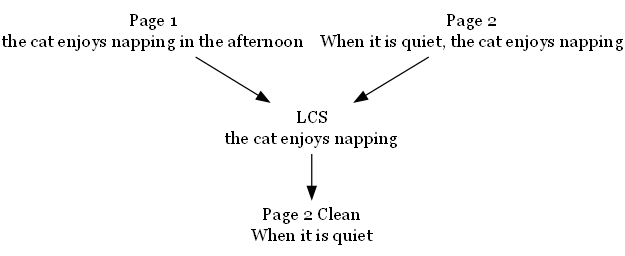
\includegraphics[width=\linewidth]{images/svg_graph} 

}

\caption{Longest Common Substring Diagram}\label{fig:lcs}
\end{figure}

The PTXQC package (Bielow et al.) implements LCS using dynamic programming, as opposed to the suffix tree method (which has not been implemented in CRAN).
Their dynamic programming process is described below.
This method creates an empty matrix, where the number of rows correspond to the length of the first string, and the number of columns correspond to the length of the second string.
Thus, the first cell would correspond to the first character of both strings, and so on.
If the characters match and it is the first row or column, then the cell gets a value of 1.
If the characters match and it is not the first row or column, the the cell receives the value of the (i-1,j-1) cell plus one.
The first string's index for the substring of the longest length is saved.
This process is shown in Table \ref{tab:dylcs}, with two strings: ``cabbacced'' and ``bbacccade''.
The diagonal of numbers in red indicate the longest substring, beginning with `b' and ending with `c'
Thus, ``bbacc'' is identified as the LCS.

\begin{longtable}[]{@{}llllllllll@{}}
\caption{Dynamic Programming for LCS \label{tab:dylcs}}\tabularnewline
\toprule()
\_ & c & a & b & b & a & c & c & e & d \\
\midrule()
\endfirsthead
\toprule()
\_ & c & a & b & b & a & c & c & e & d \\
\midrule()
\endhead
b & 0 & 0 & \textcolor{red}{1} & 1 & 0 & 0 & 0 & 0 & 0 \\
b & 0 & 0 & 1 & \textcolor{red}{2} & 0 & 0 & 0 & 0 & 0 \\
a & 0 & 1 & 0 & 0 & \textcolor{red}{3} & 0 & 0 & 0 & 0 \\
c & 1 & 0 & 0 & 0 & 0 & \textcolor{red}{4} & 1 & 0 & 0 \\
c & 1 & 0 & 0 & 0 & 0 & 1 & \textcolor{red}{5} & 0 & 0 \\
c & 1 & 0 & 0 & 0 & 0 & 1 & 2 & 0 & 0 \\
a & 0 & 1 & 0 & 0 & 1 & 0 & 0 & 0 & 0 \\
d & 0 & 0 & 0 & 0 & 0 & 0 & 0 & 0 & 1 \\
e & 0 & 0 & 0 & 0 & 0 & 0 & 0 & 0 & 0 \\
\bottomrule()
\end{longtable}

The Longest Common Substring method is able to handle the issues found in the First n Character method, which is demonstrated in Table \ref{tab:issues}.
If notes are deleted, the LCS method can identify the substring from the previous notes, despite the large edit distance that would prevent removal in the First n Character method.
If new notes are inserted in the middle of previous notes, the First n Character method would compare the Page 1's notes with the red text of the Page 2 notes shown in the second row, resulting in an edit distance that would prevent removal.
With the LCS method, the first substring ``The cat ran'' could be identified and removed, then in a second iteration, the second substring of ``up the tree'' can also be removed, leaving only the new text.
In the case of duplication, the First n Character method would be able to identify the first iteration of text that matches Page 1 and remove it; but it would not be able to identify the second occurrence of the text.
As before, the LCS method would be able to identify both instances through two iterations, and remove all Page 1 text.

\begin{longtable}[]{@{}
  >{\raggedright\arraybackslash}p{(\columnwidth - 8\tabcolsep) * \real{0.1860}}
  >{\raggedright\arraybackslash}p{(\columnwidth - 8\tabcolsep) * \real{0.1860}}
  >{\raggedright\arraybackslash}p{(\columnwidth - 8\tabcolsep) * \real{0.2093}}
  >{\raggedright\arraybackslash}p{(\columnwidth - 8\tabcolsep) * \real{0.2093}}
  >{\raggedright\arraybackslash}p{(\columnwidth - 8\tabcolsep) * \real{0.2093}}@{}}
\caption{LCS Comparison for FNC Issues \label{tab:issues}}\tabularnewline
\toprule()
\begin{minipage}[b]{\linewidth}\raggedright
Issue
\end{minipage} & \begin{minipage}[b]{\linewidth}\raggedright
Page 1
\end{minipage} & \begin{minipage}[b]{\linewidth}\raggedright
Page 2
\end{minipage} & \begin{minipage}[b]{\linewidth}\raggedright
LCS
\end{minipage} & \begin{minipage}[b]{\linewidth}\raggedright
Edit Distance
\end{minipage} \\
\midrule()
\endfirsthead
\toprule()
\begin{minipage}[b]{\linewidth}\raggedright
Issue
\end{minipage} & \begin{minipage}[b]{\linewidth}\raggedright
Page 1
\end{minipage} & \begin{minipage}[b]{\linewidth}\raggedright
Page 2
\end{minipage} & \begin{minipage}[b]{\linewidth}\raggedright
LCS
\end{minipage} & \begin{minipage}[b]{\linewidth}\raggedright
Edit Distance
\end{minipage} \\
\midrule()
\endhead
Deletion & The cat ran up the tree & The cat ran & The cat ran & 12 \\
Insertion & The cat ran up the tree & \textcolor{red}{The cat ran, chased by a} dog, up the tree & (The cat ran)(up the tree) & 11 \\
Duplication & The cat ran up the tree & \textcolor{red}{The cat ran up the tree} The cat ran up the tree & (The cat ran up the tree)(The cat ran up the tree) & 0 \\
\bottomrule()
\end{longtable}

While the LCS method is able to solve the issues related to the First N Character method, it has some issues of its own.
If the testimony itself contains duplicate text, such as the text related to swearing in witnesses, the LCS method would remove the new text that corresponds to the later testimony.
The other issue with the LCS method is the time required when it is applied to the entire testimony.
In the validation study described below, the LCS method took approximately 30 times as long as the FNC method.

\hypertarget{hybrid-method}{%
\subsubsection{Hybrid Method}\label{hybrid-method}}

In order to compare the two methods described above, I cleaned a subset of the survey response notes to have a ``correct'' baseline with which to calculate error rates.
This dataset consists of 561 pages of `notes' (including blanks) with 35 unique participants.
30 participants were randomly selected from the larger dataset, while 5 participants were selected based on demonstrated issues with data cleaning.
The 5 selected participants included an individual who deleted almost all of the beginning notes; two individuals who pasted new notes in the middle of old notes; an individual who duplicated notes; and an individual who included the algorithm expert's trial confirmation as well as the forensic scientist's - duplicate text that should be included as the new notes.

For the FNC method, the length of the previous notes is compared to the beginning of the current page's notes.
If the edit distance is below a certain threshold, these notes are removed.
In this case, I changed the threshold with values of 0 character difference, 5 character difference, and 15 character difference (set as less than 1, less than 6, and less than 16).
In the case of LCS, a threshold must be picked for the minimum matching substring length to be considered `previous notes' and removed.
If the threshold is too small, the LCS method can identify words like ``the'' as matching previous testimony to be removed.
If the threshold is too large, the LCS method may be unable to remove substrings when new text is inserted in the middle of the old text.
Here, I tried several different character lengths: 40 characters, half the previous note length, a third of the previous note length, and a fourth of the previous note length plus 5 (to compensate for shorter strings).

I also investigated the use of a hybrid method in the hope that the FNC method could be used as a quick way to clean the simplest cases of notes, while the LCS method could be used to clean up the notes that are less clear-cut.
In order to determine which observations would need the second cleaning method, I created the plot below.

\hypertarget{notes}{%
\section{Notes}\label{notes}}

\begin{itemize}
\item
  Participants of the first study were allowed to take notes while reading through the transcripts, which are saved by page number
\item
  We would like to use this to highlight which parts of the testimonies the participants found to be important
\item
  First attempt:

  \begin{itemize}
  \tightlist
  \item
    ggplot: allows for both a gradient and transparency to be added to words based on their frequency
  \item
    graphing words of the transcript resulted in uneven spacing
  \item
    Relative frequency was computed based on the number of times the word appeared on the page
  \end{itemize}
\item
  Second attempt:

  \begin{itemize}
  \tightlist
  \item
    Using CSS instead of ggplot: can set gradient through color outputted by ggplot
  \item
    Words can be equally spaced
  \item
    Labels added with gradient scale
  \item
    Change from relative frequency of individual words to average collocation frequency per word (with collocations of length 5)
    -Include fuzzy matching for indirect matches (typos/skipped words)
  \end{itemize}
\end{itemize}

\hypertarget{study2}{%
\chapter{Jury Perception Revisited: This Time with Caricatures}\label{study2}}

\begin{itemize}
\item
  Study 2 changes can be found in Appendix \ref{study-2-changes}
\item
  When reading a transcript, experts may seem impartial when they are in fact called by the prosecution
\item
  There are few to no visuals to keep track of who is speaking, and what characters are present in a scenario
\item
  We wanted to develop a general tool that can be used in online courtroom studies, making it easier to track sides/speakers, and with versatility in terms of race/gender
\item
  Other changes:

  \begin{itemize}
  \tightlist
  \item
    combating scale compression through jury instructions before deliberation
  \item
    Fixed code design so to prevent copy-paste error
  \item
    Comparing Likert scales to quantitative scales
  \item
    Adding scenario id to database at beginning of test
  \end{itemize}
\item
  Reliability: Questions regarding the consistency of the comparison

  \begin{itemize}
  \tightlist
  \item
    How often to you think the firearms examiner makes mistakes?

    \begin{itemize}
    \tightlist
    \item
      {[}blank{]} out of {[}blank{]} bullet comparisons
    \end{itemize}
  \item
    How often to you think the algorithm makes mistakes?

    \begin{itemize}
    \tightlist
    \item
      {[}blank{]} out of {[}blank{]} bullet comparisons
    \end{itemize}
  \item
    If other examiners were asked to make the same bullet comparison, how many do you believe would agree with the firearms examiner

    \begin{itemize}
    \tightlist
    \item
      {[}blank{]} out of {[}blank{]} examiners would agree with Smith's results of bullet comparison
    \end{itemize}
  \item
    If the algorithm were re-run on the same bullet comparison, how many times do you believe the algorithm would agree with these results?

    \begin{itemize}
    \tightlist
    \item
      {[}blank{]} out of {[}blank{]} runs would agree with the results of the bullet comparison
    \end{itemize}
  \item
    Scientificity: can directly compare to each other, or have a non-scientific portion to compare to

    \begin{itemize}
    \tightlist
    \item
      Did you find the algorithm or the bullet comparison to be more scientific?
    \item
      Compared to the case description, how would you rate the scientificity of the bullet comparison
    \end{itemize}
  \item
    How much would you be willing to bet that the crime scene bullet (did/did not) match Cole's gun?
  \end{itemize}
\item
  Clarify if the examiner used the algorithm before or after their initial comparison.
\end{itemize}

\hypertarget{conclusion-1}{%
\chapter*{Conclusion}\label{conclusion-1}}
\addcontentsline{toc}{chapter}{Conclusion}

If we don't want Conclusion to have a chapter number next to it, we can add the \texttt{\{-\}} attribute.

\textbf{More info}

And here's some other random info: the first paragraph after a chapter title or section head \emph{shouldn't be} indented, because indents are to tell the reader that you're starting a new paragraph. Since that's obvious after a chapter or section title, proper typesetting doesn't add an indent there.

\appendix

\hypertarget{testimony-transcripts}{%
\chapter{Testimony Transcripts}\label{testimony-transcripts}}

\hypertarget{firearm-examiner}{%
\section{Firearm Examiner}\label{firearm-examiner}}

Q: Please state your name.

A: John Smith

Q: Who do you work for? (\emph{State of {Arizona} vs. Eduardo {Vasquez} {Celaya}}, 2007, pp. 6--7)

A: The local police department

Q: What do you do for the police department? (\emph{State of {Arizona} vs. Eduardo {Vasquez} {Celaya}}, 2007, pp. 6--7)

A: I am a firearms examiner (\emph{State of {Arizona} vs. Eduardo {Vasquez} {Celaya}}, 2007, pp. 6--7)

Q: How long have you been doing that? (\emph{State of {Arizona} vs. Eduardo {Vasquez} {Celaya}}, 2007, pp. 6--7)

A: X amount of years

Q: What is a firearms examiner? (\emph{State of {Arizona} vs. Eduardo {Vasquez} {Celaya}}, 2007, pp. 6--7)

A: A firearms examiner is someone who looks at cartridge cases and bullets to determine whether they were fired in a particular firearm.

Q: What training is required to become a firearms examiner with the local police department? (\emph{State of {Arizona} vs. Eduardo {Vasquez} {Celaya}}, 2007, pp. 6--7)

A: I received my bachelor's degree in forensic science and in X year I transferred to the crime lab from the crime scene unit. (\emph{State of {Arizona} vs. Eduardo {Vasquez} {Celaya}}, 2007, pp. 6--7)
I underwent a two-year training program, which was supervised by experienced firearms examiners (\emph{State of {Florida} vs. Sheppard {Jr.}}, 2012, pp. 798--799);
I've toured manufacturing facilities and saw how firearms and ammunition were produced; and I've attended several national and regional meetings of firearms examiners.(\emph{State of {Arizona} vs. Eduardo {Vasquez} {Celaya}}, 2007, pp. 6--7)

Q: And during the course of your career, were you tested in proficiency to make sure.. you were still conducting appropriate examinations? (\emph{State of {Florida} vs. Sheppard {Jr.}}, 2012, pp. 798--799)

A: Yes. I have undergone annual proficiency examinations.(\emph{State of {Florida} vs. Sheppard {Jr.}}, 2012, pp. 798--799)

Q: Is the local police department lab accredited? (\emph{State of {Arizona} vs. Eduardo {Vasquez} {Celaya}}, 2007, pp. 6--7)

A: Yes, it is accredited by ASCLID/LAB (\emph{State of {Arizona} vs. Eduardo {Vasquez} {Celaya}}, 2007, pp. 6--7)

Q: And in addition to what you just told us, do you have other qualifications? (\emph{The {People} of the {State} of {Illinois} v. Eugene {Banks}, et. al}, n.d., p. 2)

A: Yes, I do.(\emph{The {People} of the {State} of {Illinois} v. Eugene {Banks}, et. al}, n.d., p. 2)

Q: Can you tell us what those are? (\emph{The {People} of the {State} of {Illinois} v. Eugene {Banks}, et. al}, n.d., p. 2)

A: Yes. I received training in the use of a bullet matching algorithm.
This is an algorithm that evaluates the characteristics of two fired bullets, in order to produce a score for the similarity of the bullets, where more similar bullets are more likely to have been fired from the same gun.
I attended a workshop on the algorithm on {[}DATE{]}, held by CSAFE -- Center for Statistics and Applications in Forensic Evidence.
This involved use of the algorithm alongside my personal judgement.
I found that my conclusion was reflected in the similarity score produced by the algorithm in all \#\# cases.

Q: Where does the bullet matching algorithm come from? (\emph{The {People} of the {State} of {Michigan} v. Andrew {Mack} {Johnson}, {Jr.}}, 2018, p. 5)

A: It was created by \_\_\_\_\_. (\emph{The {People} of the {State} of {Michigan} v. Andrew {Mack} {Johnson}, {Jr.}}, 2018, p. 5)

Q: How long has the state police been using the bullet matching algorithm? (\emph{The {People} of the {State} of {Michigan} v. Andrew {Mack} {Johnson}, {Jr.}}, 2018, p. 5)

A: They have been using it since \#\#\#.

Q: Have you testified in court previously regarding the bullet matching algorithm? (\emph{The {People} of the {State} of {Michigan} v. Andrew {Mack} {Johnson}, {Jr.}}, 2018, p. 5)

A: Yes, I have, approximately \#\# times. (\emph{The {People} of the {State} of {Michigan} v. Andrew {Mack} {Johnson}, {Jr.}}, 2018, p. 5)

Q: Have you, as a firearms examiner, have you testified about opinions, given your opinion about the results of your testing? (\emph{The {People} of the {State} of {Michigan} v. Andrew {Mack} {Johnson}, {Jr.}}, 2018, p. 5)

A: Yes, I have. (\emph{The {People} of the {State} of {Michigan} v. Andrew {Mack} {Johnson}, {Jr.}}, 2018, p. 5)

Prosecution: Your Honor, at this time I would ask that XXX be qualified as an expert in the field of firearms identification subject to cross examination. (\emph{The {People} of the {State} of {Illinois} v. Eugene {Banks}, et. al}, n.d., p. 4)

Court: Any cross on their credentials? (\emph{The {People} of the {State} of {Illinois} v. Eugene {Banks}, et. al}, n.d., p. 4)

Defense: No, Your Honor (\emph{The {People} of the {State} of {Illinois} v. Eugene {Banks}, et. al}, n.d., p. 4)

Court: This witness is an expert in the area of firearms identification.
They can testify to their opinions as well as facts.
Go ahead.(\emph{The {People} of the {State} of {Illinois} v. Eugene {Banks}, et. al}, n.d., p. 4)

Q: What work did you do on this case? (\emph{State of {Arizona} vs. Eduardo {Vasquez} {Celaya}}, 2007, p. 8)

A: I was asked to compare a bullet from the crime scene to a test fire from XX gun.(\emph{State of {Arizona} vs. Eduardo {Vasquez} {Celaya}}, 2007, p. 8)

Q: Did you examine how many lands and grooves the bullet had? (\emph{State of {Arizona} vs. Eduardo {Vasquez} {Celaya}}, 2007, pp. 17--18)

A: Yes. (\emph{State of {Arizona} vs. Eduardo {Vasquez} {Celaya}}, 2007, pp. 17--18)

Q: Can you explain for the jury what that means? (\emph{State of {Arizona} vs. Eduardo {Vasquez} {Celaya}}, 2007, pp. 17--18)

A: Yes\ldots{} In the interior of a barrel there are raised portions called lands and depressed areas called grooves.
When a bullet passes down the barrel, a bullet will spin and that gives it stability and accuracy over a distance.
Those raised areas are designed by the manufacturer.
They're cut into the barrel.
And each particular file has a different combination of lands and grooves.
But essentially what those lands do will grip a bullet and spin it and as that bullet passes down the barrel, it scratches the random imperfections of that barrel into the bullet.(\emph{State of {Arizona} vs. Eduardo {Vasquez} {Celaya}}, 2007, pp. 17--18)

Q: Now, for these bullets, you counted up the lands and grooves and determined the direction of the twist, correct? (\emph{State of {Arizona} vs. Eduardo {Vasquez} {Celaya}}, 2007, pp. 17--18)

A: Yes. This bullet had six lands. And the interior of the barrel, the barrel will either twist right or it will twist left.
And this particular case, the barrel twists right.
And you can see that by looking at the bullet.
If you look at the base of the bullet, either it goes to the left or goes to the right.(\emph{State of {Arizona} vs. Eduardo {Vasquez} {Celaya}}, 2007, pp. 17--18)

---Test-fired bullets admitted into evidence---

Q: Can you describe the process of obtaining these test-fired bullets?

A: The test-fired bullets came from a test fire of XX gun.

Q: You mentioned test firings, can you explain what that means? (\emph{The {People} of the {State} of {Illinois} v. Eugene {Banks}, et. al}, n.d., p. 6)

A: In test firing first what I would do is make sure the firearm is safe to actually test fire.
Then I would use lab ammunition and I would test fire it, meaning that I'm creating a fired bullet.
Typically you do two at a time.
That way you have a fired bullet to compare to another fired bullet. (\emph{The {People} of the {State} of {Illinois} v. Eugene {Banks}, et. al}, n.d., p. 6)

Q: Would you then have taken the test firings you created and did you compare those test firings to the fired evidence that you had also received? (\emph{The {People} of the {State} of {Illinois} v. Eugene {Banks}, et. al}, n.d., p. 6)

A: Yes. First what I would do is compare my test shot to test shot.
I'm looking for a detailed microscopic pattern.
Once I have done that then I would compare it to the fired evidence.(\emph{The {People} of the {State} of {Illinois} v. Eugene {Banks}, et. al}, n.d., p. 6)

Q: And how about the number of lands and direction of twist for the test fires? (\emph{State of {Arizona} vs. Eduardo {Vasquez} {Celaya}}, 2007, pp. 19--20)

A: It also had six lands, and twisted to the right (\emph{State of {Arizona} vs. Eduardo {Vasquez} {Celaya}}, 2007, pp. 19--20)

Q: Okay. Now, did you compare the test-fired bullets to the fired evidence under the comparison microscope? (\emph{State of {Arizona} vs. Eduardo {Vasquez} {Celaya}}, 2007, pp. 19--20)

A: Yes, I did. (\emph{State of {Arizona} vs. Eduardo {Vasquez} {Celaya}}, 2007, pp. 19--20)

Q: What is your conclusion? (\emph{State of {Arizona} vs. Eduardo {Vasquez} {Celaya}}, 2007, pp. 19--20)

A: I found that there were sufficient individualizing characteristics to conclude that the two bullets were fired from the same barrel.

Q: How were you able to conclude that? (\emph{State of {Arizona} vs. Eduardo {Vasquez} {Celaya}}, 2007, pp. 19--20)

A: I placed them under the comparison microscope, and I roll the bullet around 'til I can see the agreement in a particular area, unique surface contour that has sufficient agreement.
At that point, when I've seen that, I start to rotate the bullets around and I look at all the different lands and grooves, impressions, for that unique detail.
When I can see those, that agreement on multiple areas of the bullet, I identify the bullet as having sufficient agreement.(\emph{State of {Arizona} vs. Eduardo {Vasquez} {Celaya}}, 2007, pp. 19--20)

Q: Did you use an algorithm to compare these bullets as well?

A: Yes, I used the algorithm to compare the two test fires to each other.
I also used the algorithm to compare the better-marking test fire to the fired evidence that I received.

Q: Could you explain how this algorithm compares bullets?

A: The algorithm uses 3D measurements to make a comparison between the surface contours of each of the lands on each bullet.
These comparisons result in a match score between 0 and 1, where 1 indicates a clear match, and 0 indicates that there is not a match.
The bullet is aligned based on the maximum agreement between the lands, and the average match score for the lands is computed.
This average score gives an overall match score for the entire bullet.

Q: What was the match score between the two test-fired bullets?

A: The match score was 0.9-.

Q: What was the match score between the better-marked test fire bullet and the fired evidence?

A: The match score was 0.XX.

Q: What does this match score indicate about the bullets?

A: The match score indicates that there is substantial similarity between the two bullets, which suggests that they were most likely fired from the same barrel.

Q: Now, how many times have you compared bullets to determine if they were fired from the same gun? (\emph{State of {Arizona} vs. Eduardo {Vasquez} {Celaya}}, 2007, pp. 19--20)

A: I'd say thousands. (\emph{State of {Arizona} vs. Eduardo {Vasquez} {Celaya}}, 2007, pp. 19--20)

Q: And do you ever see two bullets that have agreement in every area of the bullet? (\emph{State of {Arizona} vs. Eduardo {Vasquez} {Celaya}}, 2007, pp. 19--20)

A: No.~
The firing process of a firearm is dynamic, kind of like a contained explosion.
When the firing pin hits the primer, which is basically the initiator, what gets it going, it will explode, bur the gun powder inside the casing, and the bullet will travel down the barrel, picking up the microscopic imperfections of the barrel, and the cartridge case will slam rearward against the support mechanism.
During that dynamic process, each time it happens, a bullet will be marked slightly differently from one to the next. (\emph{State of {Arizona} vs. Eduardo {Vasquez} {Celaya}}, 2007, pp. 19--20)

Q: When you reached a conclusion, did you write up a report? (\emph{State of {Arizona} vs. Eduardo {Vasquez} {Celaya}}, 2007, p. 23)

A: Yes, I did. (\emph{State of {Arizona} vs. Eduardo {Vasquez} {Celaya}}, 2007, p. 23)

Q: Is it the local police department's protocol to have somebody else who's a firearms tool mark examiner in your lab review that report, review your work, and determine if it's correct? (\emph{State of {Arizona} vs. Eduardo {Vasquez} {Celaya}}, 2007, p. 23)

A: Yes. (\emph{State of {Arizona} vs. Eduardo {Vasquez} {Celaya}}, 2007, p. 23)

Q: That's what we call peer review? (\emph{State of {Arizona} vs. Eduardo {Vasquez} {Celaya}}, 2007, p. 23)

A: Peer review, yes. (\emph{State of {Arizona} vs. Eduardo {Vasquez} {Celaya}}, 2007, p. 23)

Q: Thank you, no further questions. (\emph{State of {Arizona} vs. Eduardo {Vasquez} {Celaya}}, 2007, p. 40)

--Cross examination----

Q: Now, are you telling the jury today that in your opinion there's only one gun in the entire world that could have produced the markings that you saw on these bullets? (\emph{State of {Arizona} vs. Eduardo {Vasquez} {Celaya}}, 2007, p. 65)

A: I'm saying that the probability that the two markings were made by different sources is so small that it is negligible. (Office of Legal Policy, 2020, p. 2) (\emph{State of {Arizona} vs. Eduardo {Vasquez} {Celaya}}, 2007, p. 65)

Q: Exclusive to any other gun? (\emph{State of {Arizona} vs. Eduardo {Vasquez} {Celaya}}, 2007, p. 65)

A: I obviously haven't tested every other gun, but it is a practical impossibility. (\emph{State of {Arizona} vs. Eduardo {Vasquez} {Celaya}}, 2007, p. 65)

Q: That's your opinion. And your opinion, by the way, is subjective, right, and it's based on your experience? (\emph{State of {Arizona} vs. Eduardo {Vasquez} {Celaya}}, 2007, pp. 72--73)

A: Based on my training and experience, yes. (\emph{State of {Arizona} vs. Eduardo {Vasquez} {Celaya}}, 2007, pp. 72--73)

Q: Is there something fixed about the amount of what has to be found to constitute sufficient agreement? (\emph{{U.S.} Vs. {Harris}}, 2016, pp. 4459--4460)

A: No, there is not a fixed amount or a numerical value. (\emph{{U.S.} Vs. {Harris}}, 2016, pp. 4459--4460)

Q: How long did you say you've been trained in the bullet matching algorithm? (\emph{The {People} of the {State} of {Michigan} v. Andrew {Mack} {Johnson}, {Jr.}}, 2018, p. 19 - 21)

A: Since XXX (\emph{The {People} of the {State} of {Michigan} v. Andrew {Mack} {Johnson}, {Jr.}}, 2018, p. 19 - 21)

Q: Okay. So that's fairly new; is that fair to say? (\emph{The {People} of the {State} of {Michigan} v. Andrew {Mack} {Johnson}, {Jr.}}, 2018, p. 19 - 21)

A: It is still fairly new, yes. (\emph{The {People} of the {State} of {Michigan} v. Andrew {Mack} {Johnson}, {Jr.}}, 2018, p. 19 - 21)

Q: The software uses modeling; is that correct? (\emph{The {People} of the {State} of {Michigan} v. Andrew {Mack} {Johnson}, {Jr.}}, 2018, p. 19 - 21)

A: Yes, it does. (\emph{The {People} of the {State} of {Michigan} v. Andrew {Mack} {Johnson}, {Jr.}}, 2018, p. 19 - 21)

Q: You, personally, don't know the source code; is that correct? (\emph{The {People} of the {State} of {Michigan} v. Andrew {Mack} {Johnson}, {Jr.}}, 2018, p. 19 - 21)

A: That's correct.(\emph{The {People} of the {State} of {Michigan} v. Andrew {Mack} {Johnson}, {Jr.}}, 2018, p. 19 - 21)

Q: And, in fact, you, personally, would not be able to tell us the specific math that goes into this program; is that fair to say? (\emph{The {People} of the {State} of {Michigan} v. Andrew {Mack} {Johnson}, {Jr.}}, 2018, p. 19 - 21)

A: We did receive training on what the math is doing. (\emph{The {People} of the {State} of {Michigan} v. Andrew {Mack} {Johnson}, {Jr.}}, 2018, p. 19 - 21)

The Court: Terry Smith, the jury has asked me to forward this question to you. Answer if you're able.
To what percentage is the science accurate is the first question. And then I think the rest of that explanation of that question goes on to say, to determine that the bullets were fired from the same firearm, are you 100 percent sure? (\emph{State of {Arizona} vs. Eduardo {Vasquez} {Celaya}}, 2007, pp. 100--101)

A: My opinion, I am 100 percent sure that these bullets were fired from this firearm.
There is a published error rate for firearms examiners.
The positive identification is less than two percent.
I believe it's about 1.5 to 1.9. That's just a general number that's out there.(\emph{State of {Arizona} vs. Eduardo {Vasquez} {Celaya}}, 2007, pp. 100--101)
The false negative identification rate is less than three percent. (Chumbley et al., 2021)

\hypertarget{algorithm-expert}{%
\section{Algorithm Expert}\label{algorithm-expert}}

Inspired by \emph{State of {Arizona} vs. Eduardo {Vasquez} {Celaya}} (2007), \emph{The {People} of the {State} of {Illinois} v. Eugene {Banks}, et. al} (n.d.), \emph{The {People} of the {State} of {Michigan} v. Andrew {Mack} {Johnson}, {Jr.}} (2018), \emph{{U.S.} Vs. {Harris}} (2016), \emph{State of {Florida} vs. Sheppard {Jr.}} (2012), Hare et al. (2017), Vanderplas et al. (2020), and Perlin (2012). Should create citations by line as above.

Q: Please state your name.

A: Adrian/Avery Jones

Q: Who do you work for? (\emph{State of {Arizona} vs. Eduardo {Vasquez} {Celaya}}, 2007, pp. 6--7)

A: XXX place

Q: What is your current occupation?

A: XXX

Q: How long have you been doing that? (\emph{State of {Arizona} vs. Eduardo {Vasquez} {Celaya}}, 2007, pp. 6--7)

A: X amount of years

Q: What training is required to hold this occupation? (\emph{State of {Arizona} vs. Eduardo {Vasquez} {Celaya}}, 2007, pp. 6--7)

A: I have a Ph.D.~in XX, and have spent X time developing the bullet matching algorithm algorithms.
I have spent X years collaborating with firearms examiners during the development and rollout of this algorithm.

Q: Are you familiar with the bullet matching algorithm?

A: Yes. I was involved in the development of the algorithm.

Prosecution: Your Honor, at this time I would ask that XXX be qualified as an expert in the bullet matching algorithm subject to cross examination.
Court: Any cross on their credentials? (\emph{The {People} of the {State} of {Illinois} v. Eugene {Banks}, et. al}, n.d., p. 4)

Defense: No, Your Honor (\emph{The {People} of the {State} of {Illinois} v. Eugene {Banks}, et. al}, n.d., p. 4)

Court: This witness is an expert in the area of the bullet matching algorithm. They can testify to their opinions as well as facts. (\emph{The {People} of the {State} of {Illinois} v. Eugene {Banks}, et. al}, n.d., p. 4)

Q: How many times have you testified regarding this bullet matching algorithm?

A: XX times.

Q: Could you describe how this bullet matching algorithm compares bullets?

A: Yes. For certain types of guns, the barrel will have lands and grooves, known as rifling.
This rifling spins the bullet in order to make its trajectory more stable. Due to the manufacturing process, this rifling can produce identifiable markings on the bullet, based on random differences between barrels.
Because of these random imperfections, the striation marks left on bullets can be compared in order to determine if it is likely that they were fired from the same gun.

(Description based on Hare et al. (2017))
The first step is to determine where the lands on the bullet are located.
These lands will be the sunken area that contains the striation marks between the smoother grooves.
3D scans are then taken for each land, and the `shoulders', or area transitioning from the land to the groove, is excluded from the analysis.

Next, a stable area of the 3D scan containing the striations is selected, and a cross-section of this area is used to show the striations along with the topology of the region.
A smoothing function is applied to remove some of the imaging noise from the 3D scan, leaving the striae intact.
A second smooth is subtracted from the striations in order to remove the curvature of the region, leaving only the striae -- this is what we call a signature.
The signature for the two bullets being compared are aligned such that the best fit between the two signatures is achieved.
The striation marks between the two signatures are then compared by evaluating how many of the high points and low points correspond.
The algorithm can calculate the number of consecutively matching striations (CMS), or consecutively matching high points and low points -- these are features used directly by some examiners to characterize the strength of a match.
It also calculates the cross correlation between the two signatures, which is a numerical measure of the similarity between the two lands ranging between --1 and 1.

These traits are combined using what is known as a random forest.
Each forest is composed of decision trees, which use a subset of the observed values in order to make a decision about whether or not the bullets constitute a match.
The other observations are held out in order to determine an error rate.
When the random forest makes a prediction, each decision tree ``votes'', producing a numerical value between 0 and 1 corresponding to the percentage of trees which evaluate the features as being sufficiently similar to have come from the same source.

Q: Have you tested this algorithm?

A: Yes.
This algorithm was tested and validated on a number of different test sets of bullet scans.
It was found that, as long as there are sufficient marks on the bullet, the algorithm could successfully distinguish between bullets fired by the same gun and those fired from different guns.
Examiners' visual comparisons are also limited by the presence or absence of individualizing marks.
Two test sets were using consecutively rifled barrels, which should be the most difficult to assess, and it was shown that the algorithm could distinguish between the bullets fired from two separate guns with complete accuracy. (Vanderplas et al., 2020)

Q: Can this algorithm be used on XX bullets fired from an XX firearm, such as the firearm in question for this case?
(Discussion of limitations (\emph{The {People} of the {State} of {Michigan} v. Andrew {Mack} {Johnson}, {Jr.}}, 2018, p. 11))

A: Yes, this algorithm can be used on these types of bullets, given that this type of firearm marks well.

Q: Has this algorithm been published? (Perlin (2012) for importance of publication)

A: Yes. The algorithm and its process has been discussed in peer reviewed journals such as Law, Probability, and Risk, The Annals of Applied Statistics, and Forensic Science International.
The algorithm is also open source, which means that the full source code, documentation, and numerical weights are available online for anyone to examine.

--Cross examination----

Q: How long has the bullet matching algorithm been used in court cases? (\emph{The {People} of the {State} of {Michigan} v. Andrew {Mack} {Johnson}, {Jr.}}, 2018, p. 19 - 21)

A: Since XXX

Q: Okay. So that's fairly new; is that fair to say? (\emph{The {People} of the {State} of {Michigan} v. Andrew {Mack} {Johnson}, {Jr.}}, 2018, p. 19 - 21)

A: It is still fairly new, yes. (\emph{The {People} of the {State} of {Michigan} v. Andrew {Mack} {Johnson}, {Jr.}}, 2018, p. 19 - 21)

Q: This algorithm requires some decision making on the part of the operator, such as how much the signature is smoothed and what part of the bullets are inputted into the system, correct? (subjective aspects (\emph{The {People} of the {State} of {Michigan} v. Andrew {Mack} {Johnson}, {Jr.}}, 2018, p. 21))

A: Yes, there are certain parameters which must be specified, but the system defaults are usually sufficient and have been validated with a number of different firearms and ammunition types.
There are also operating protocols for determining which parts of the bullet are scanned, so while this process is manual, there are clear criteria and the associated variability from scanning is well understood, and published in Forensic Science International.

Q: Can this algorithm be applied to all bullets? (gun specific/issues with damaged bullets)

A: No, the algorithm only works on traditionally rifled bullets which are largely undamaged.
The algorithm has not been validated to work on seriously damaged or fragmented bullets.

\hypertarget{study-2-changes}{%
\chapter{Study 2 Changes}\label{study-2-changes}}

\hypertarget{cautions-against-expert-witnesses}{%
\section{Cautions Against Expert Witnesses}\label{cautions-against-expert-witnesses}}

\hypertarget{jury-instructions}{%
\subsection{Jury Instructions}\label{jury-instructions}}

You have heard testimony from Terry Smith and Adrian Jones who have testified to opinions and the reasons for their opinions. This opinion testimony is allowed because of the education or experience of this witness.
Such opinion testimony should be judged like any other testimony.
You may accept or reject it, and give it as much weight as you think it deserves, considering the witness's education and experience, the reasons given for the opinion, and all the other evidence in the case. (United States Courts for the Ninth Circuit, 2019)

\hypertarget{opinion-witness}{%
\subsection{Opinion Witness}\label{opinion-witness}}

United States Courts for the Ninth Circuit (2019) suggests that witnesses should not be qualified as experts, as it may cause the jury to place undue weight in their testimony. Instead, Richey (1994) implements the term ``opinion witness'' in the place of ``expert witness''. This practice has been adopted in our revised testimony, when qualifying the witness based on experience and education.

\hypertarget{cross-examination}{%
\subsection{Cross Examination}\label{cross-examination}}

The strength of evidence (``the probability that the two markings were made by different sources is so small that it is negligible'') was moved from the cross examination to the direct examination, since this strength of evidnece should be introduced by the prosecution. Additional testimony regarding subjectivity was added to the cross examination as well, from (\emph{{U.S.} Vs. {Harris}}, 2016, p. 54):

Q: You have a criterion in you head, a subjective criterion, of what will constitute an identification. Is that correct?

A: Yes.

Q: All right. If we brought three more people in, would their subjective criterion in their head be identical to yours?

A: They would look for that same sufficient agreement. However, based on their training and experience on difficult comparisons, they may or may not come to the same decision.

Q: Right. But they also could reach the same decision but have a different subjective criterion than you. Is that fair?

A: They may, possibly. I don't know. I can't speak for other examiners.

Additional testimony was also added to address the distinction between evidence that the gun was at the crime scene, and evidence that Cole was at the crime scene (\emph{State of {Florida} vs. Sheppard {Jr.}}, 2012, p. 831):

Q: You can't tell us anything about who shot the firearm, correct?

A: That is correct.

\hypertarget{clarifying-sides}{%
\section{Clarifying Sides}\label{clarifying-sides}}

To make sure individuals are clear on who the firearms examiner is testifying for, testimony was added related to the calling and the swearing in of the witness. The testimony below is from \emph{The {People} of the {State} of {Michigan} v. Andrew {Mack} {Johnson}, {Jr.}} (2018).

Court: Your next witness, please.

Prosecution: The People would call John Smith.

Court: Hello.

Smith: Hi

Court: Would you raise your right hand for me? Do you sear the testimony you're about to give will be the truth, the whole truth, nothing but the truth, under penalty of perjury?

Smith: I do.

Court: Please be seated. State your full name for the record and spell your last name.

Witness: My name in John Smith, last name S-m-i-t-h

\hypertarget{images}{%
\section{Images}\label{images}}

In order to clarify the speakers in the testimony and create a more engaging environment, we implemented character drawings (by Richy Meleus) to represent various actors that may be present in the courtroom. These characters' faces and clothing are largely exchangeable, allowing for a large combination of clothing and characteristics.

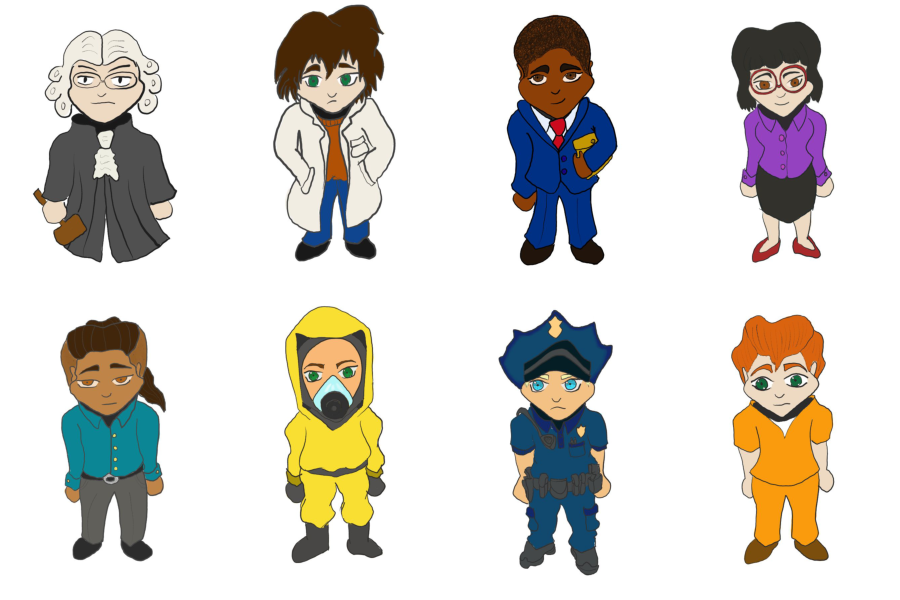
\includegraphics[width=\linewidth]{thesis_files/figure-latex/demo_evidence-1}

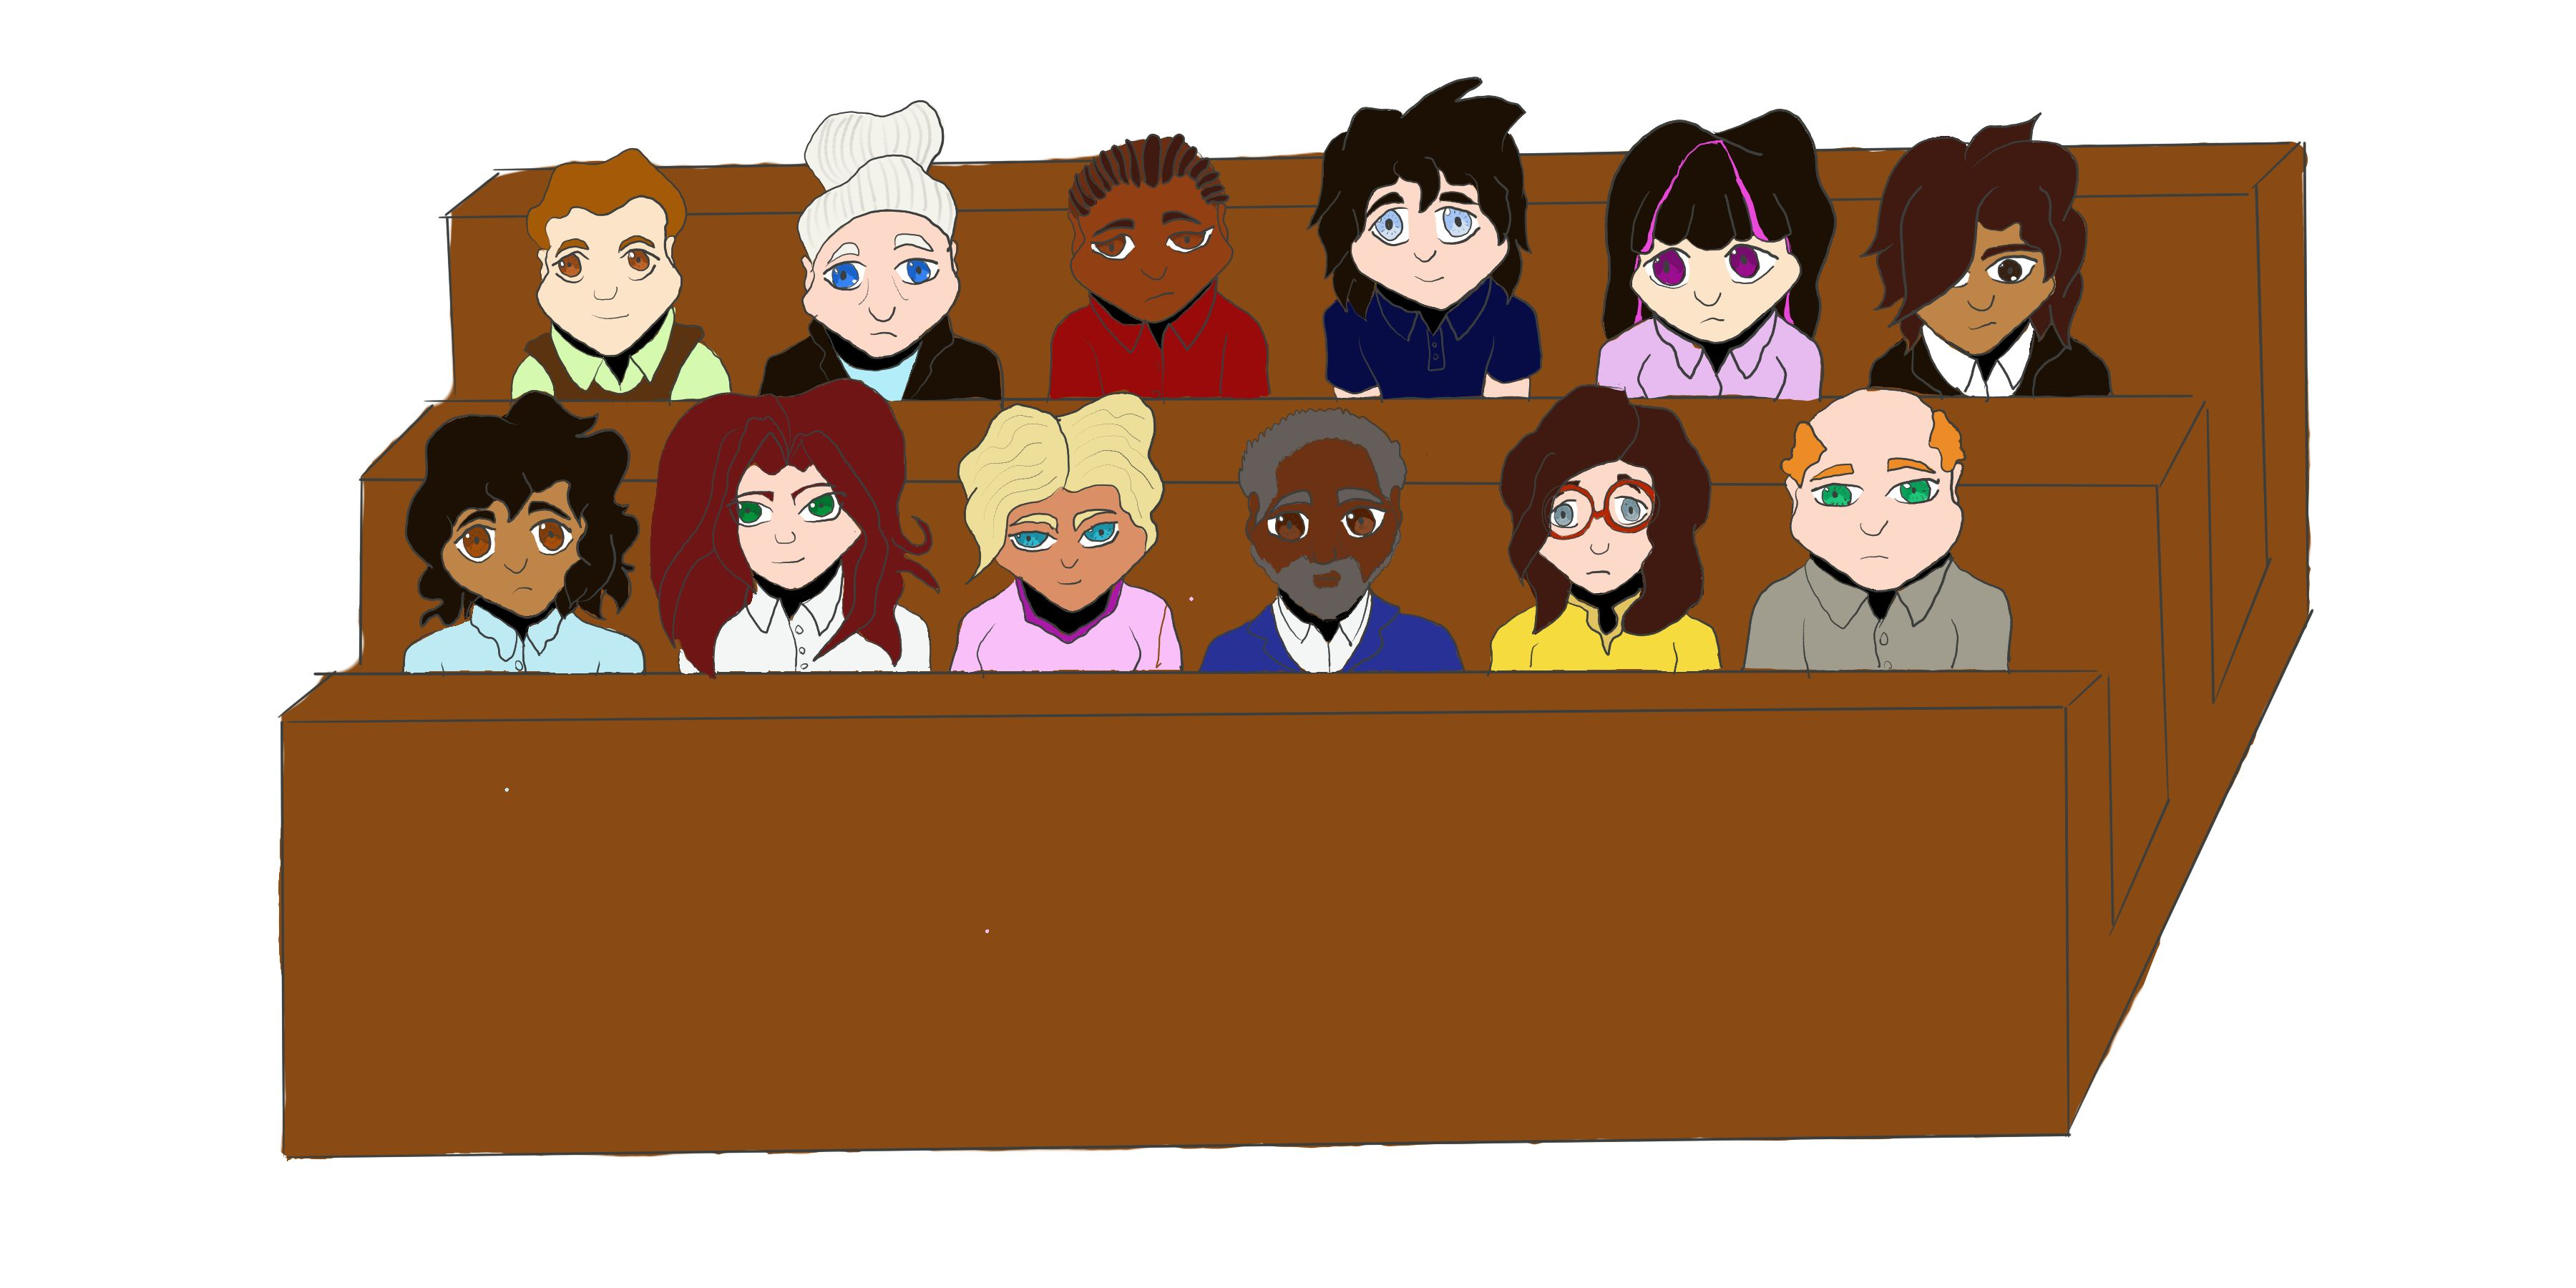
\includegraphics[width=\linewidth]{images/Jury}

\hypertarget{colophon}{%
\chapter*{Colophon}\label{colophon}}
\addcontentsline{toc}{chapter}{Colophon}

This document is set in \href{https://github.com/georgd/EB-Garamond}{EB Garamond}, \href{https://github.com/adobe-fonts/source-code-pro/}{Source Code Pro} and \href{http://www.latofonts.com/lato-free-fonts/}{Lato}. The body text is set at 11pt with \(\familydefault\).

It was written in R Markdown and \(\LaTeX\), and rendered into PDF using \href{https://github.com/benmarwick/huskydown}{huskydown} and \href{https://github.com/rstudio/bookdown}{bookdown}.

This document was typeset using the XeTeX typesetting system, and the \href{http://staff.washington.edu/fox/tex/}{University of Washington Thesis class} class created by Jim Fox. Under the hood, the \href{https://github.com/UWIT-IAM/UWThesis}{University of Washington Thesis LaTeX template} is used to ensure that documents conform precisely to submission standards. Other elements of the document formatting source code have been taken from the \href{https://github.com/stevenpollack/ucbthesis}{Latex, Knitr, and RMarkdown templates for UC Berkeley's graduate thesis}, and \href{https://github.com/suchow/Dissertate}{Dissertate: a LaTeX dissertation template to support the production and typesetting of a PhD dissertation at Harvard, Princeton, and NYU}

The source files for this thesis, along with all the data files, have been organised into an R repository, which is available at \url{https://github.com/rachelesrogers/UNL_Thesis}.

This version of the thesis was generated on 2023-05-15 13:01:37.

The computational environment that was used to generate this version is as follows:

\begin{verbatim}
## - Session info -------------------------------------------
##  setting  value
##  version  R version 4.2.1 (2022-06-23 ucrt)
##  os       Windows 10 x64 (build 18363)
##  system   x86_64, mingw32
##  ui       RTerm
##  language (EN)
##  collate  English_United States.utf8
##  ctype    English_United States.utf8
##  tz       America/Chicago
##  date     2023-05-15
##  pandoc   2.19.2 @ C:/Program Files/RStudio/resources/app/bin/quarto/bin/tools/ (via rmarkdown)
## 
## - Packages -----------------------------------------------
##  ! package            * version    date (UTC) lib source
##    ade4                 1.7-22     2023-02-06 [1] CRAN (R 4.2.2)
##    assertthat           0.2.1      2019-03-21 [1] CRAN (R 4.2.1)
##    backports            1.4.1      2021-12-13 [1] CRAN (R 4.2.0)
##    bit                  4.0.4      2020-08-04 [1] CRAN (R 4.2.1)
##    bit64                4.0.5      2020-08-30 [1] CRAN (R 4.2.1)
##    bookdown             0.32       2023-01-17 [1] CRAN (R 4.2.2)
##    broom                1.0.0      2022-07-01 [1] CRAN (R 4.2.1)
##    cachem               1.0.6      2021-08-19 [1] CRAN (R 4.2.1)
##    callr                3.7.3      2022-11-02 [1] CRAN (R 4.2.2)
##    cellranger           1.1.0      2016-07-27 [1] CRAN (R 4.2.1)
##    checkmate            2.1.0      2022-04-21 [1] CRAN (R 4.2.1)
##    cli                  3.4.1      2022-09-23 [1] CRAN (R 4.2.2)
##    colorspace           2.0-3      2022-02-21 [1] CRAN (R 4.2.1)
##    crayon               1.5.2      2022-09-29 [1] CRAN (R 4.2.2)
##    data.table           1.14.2     2021-09-27 [1] CRAN (R 4.2.1)
##    DBI                  1.1.3      2022-06-18 [1] CRAN (R 4.2.1)
##    dbplyr               2.2.1      2022-06-27 [1] CRAN (R 4.2.1)
##    devtools           * 2.4.5      2022-10-11 [1] CRAN (R 4.2.2)
##    DiagrammeR         * 1.0.9      2022-03-05 [1] CRAN (R 4.2.3)
##    digest               0.6.29     2021-12-01 [1] CRAN (R 4.2.1)
##    dplyr              * 1.0.10     2022-09-01 [1] CRAN (R 4.2.1)
##    ellipsis             0.3.2      2021-04-29 [1] CRAN (R 4.2.1)
##    evaluate             0.20       2023-01-17 [1] CRAN (R 4.2.2)
##    fansi                1.0.4      2023-01-22 [1] CRAN (R 4.2.2)
##    farver               2.1.1      2022-07-06 [1] CRAN (R 4.2.1)
##    fastmap              1.1.0      2021-01-25 [1] CRAN (R 4.2.1)
##    fastmatch            1.1-3      2021-07-23 [1] CRAN (R 4.2.0)
##    forcats            * 0.5.2      2022-08-19 [1] CRAN (R 4.2.1)
##    formatR              1.12       2022-03-31 [1] CRAN (R 4.2.2)
##    fs                   1.5.2      2021-12-08 [1] CRAN (R 4.2.1)
##    gargle               1.2.0      2021-07-02 [1] CRAN (R 4.2.1)
##    generics             0.1.3      2022-07-05 [1] CRAN (R 4.2.1)
##    GGally             * 2.1.2      2021-06-21 [1] CRAN (R 4.2.2)
##    ggblend            * 0.0.0.9000 2022-12-16 [1] Github (mjskay/ggblend@15e7544)
##    ggdendro             0.1.23     2022-02-16 [1] CRAN (R 4.2.2)
##    ggmosaic           * 0.3.3      2021-02-23 [1] CRAN (R 4.2.1)
##    ggpcp              * 0.2.0      2022-11-17 [1] Github (heike/ggpcp@f86c04e)
##    ggplot2            * 3.4.2      2023-04-03 [1] CRAN (R 4.2.3)
##    ggrepel            * 0.9.1      2021-01-15 [1] CRAN (R 4.2.1)
##    git2r                0.30.1     2022-03-16 [1] CRAN (R 4.2.1)
##    glue                 1.6.2      2022-02-24 [1] CRAN (R 4.2.1)
##    googledrive          2.0.0      2021-07-08 [1] CRAN (R 4.2.1)
##    googlesheets4        1.0.1      2022-08-13 [1] CRAN (R 4.2.1)
##    gridExtra          * 2.3        2017-09-09 [1] CRAN (R 4.2.1)
##    gtable               0.3.1      2022-09-01 [1] CRAN (R 4.2.1)
##    haven                2.5.1      2022-08-22 [1] CRAN (R 4.2.1)
##    hms                  1.1.2      2022-08-19 [1] CRAN (R 4.2.1)
##    htmlTable            2.4.1      2022-07-07 [1] CRAN (R 4.2.1)
##    htmltools            0.5.4      2022-12-07 [1] CRAN (R 4.2.2)
##    htmlwidgets          1.6.1      2023-01-07 [1] CRAN (R 4.2.2)
##    httpuv               1.6.5      2022-01-05 [1] CRAN (R 4.2.1)
##    httr                 1.4.5      2023-02-24 [1] CRAN (R 4.2.2)
##    huskydown          * 0.0.5      2022-12-13 [1] Github (benmarwick/huskydown@addb48e)
##    jpeg               * 0.1-10     2022-11-29 [1] CRAN (R 4.2.2)
##    jsonlite             1.8.4      2022-12-06 [1] CRAN (R 4.2.2)
##    kableExtra         * 1.3.4      2021-02-20 [1] CRAN (R 4.2.2)
##    knitr              * 1.42       2023-01-25 [1] CRAN (R 4.2.2)
##    labeling             0.4.2      2020-10-20 [1] CRAN (R 4.2.0)
##    later                1.3.0      2021-08-18 [1] CRAN (R 4.2.1)
##    lattice              0.20-45    2021-09-22 [2] CRAN (R 4.2.1)
##    lazyeval             0.2.2      2019-03-15 [1] CRAN (R 4.2.1)
##    lifecycle            1.0.3      2022-10-07 [1] CRAN (R 4.2.2)
##    lubridate            1.8.0      2021-10-07 [1] CRAN (R 4.2.1)
##    magrittr             2.0.3      2022-03-30 [1] CRAN (R 4.2.1)
##    MASS                 7.3-57     2022-04-22 [2] CRAN (R 4.2.1)
##    Matrix               1.5-3      2022-11-11 [1] CRAN (R 4.2.2)
##    memoise              2.0.1      2021-11-26 [1] CRAN (R 4.2.1)
##    mime                 0.12       2021-09-28 [1] CRAN (R 4.2.0)
##    miniUI               0.1.1.1    2018-05-18 [1] CRAN (R 4.2.1)
##    modelr               0.1.9      2022-08-19 [1] CRAN (R 4.2.1)
##    munsell              0.5.0      2018-06-12 [1] CRAN (R 4.2.1)
##    nsyllable            1.0.1      2022-02-28 [1] CRAN (R 4.2.2)
##    patchwork          * 1.1.2      2022-08-19 [1] CRAN (R 4.2.1)
##    pillar               1.8.1      2022-08-19 [1] CRAN (R 4.2.1)
##    pkgbuild             1.4.0      2022-11-27 [1] CRAN (R 4.2.2)
##    pkgconfig            2.0.3      2019-09-22 [1] CRAN (R 4.2.1)
##    pkgload              1.3.2      2022-11-16 [1] CRAN (R 4.2.2)
##    plotly               4.10.0     2021-10-09 [1] CRAN (R 4.2.1)
##    plyr               * 1.8.7      2022-03-24 [1] CRAN (R 4.2.1)
##    prettyunits          1.1.1      2020-01-24 [1] CRAN (R 4.2.1)
##    processx             3.7.0      2022-07-07 [1] CRAN (R 4.2.1)
##    profvis              0.3.7      2020-11-02 [1] CRAN (R 4.2.1)
##    promises             1.2.0.1    2021-02-11 [1] CRAN (R 4.2.1)
##    ps                   1.7.1      2022-06-18 [1] CRAN (R 4.2.1)
##    PTXQC              * 1.0.14     2022-09-20 [1] CRAN (R 4.2.2)
##    purrr              * 0.3.5      2022-10-06 [1] CRAN (R 4.2.2)
##    quanteda           * 3.2.4      2022-12-08 [1] CRAN (R 4.2.2)
##    quanteda.textstats * 0.96       2022-09-19 [1] CRAN (R 4.2.2)
##    R6                   2.5.1      2021-08-19 [1] CRAN (R 4.2.1)
##    R6P                  0.3.0      2022-10-02 [1] CRAN (R 4.2.2)
##    RColorBrewer         1.1-3      2022-04-03 [1] CRAN (R 4.2.0)
##    Rcpp                 1.0.9      2022-07-08 [1] CRAN (R 4.2.1)
##  D RcppParallel         5.1.6      2023-01-09 [1] CRAN (R 4.2.2)
##    readr              * 2.1.2      2022-01-30 [1] CRAN (R 4.2.1)
##    readtext           * 0.81       2021-07-14 [1] CRAN (R 4.2.2)
##    readxl               1.4.1      2022-08-17 [1] CRAN (R 4.2.1)
##    remotes              2.4.2      2021-11-30 [1] CRAN (R 4.2.3)
##    reprex               2.0.2      2022-08-17 [1] CRAN (R 4.2.1)
##    reshape              0.8.9      2022-04-12 [1] CRAN (R 4.2.1)
##    reshape2             1.4.4      2020-04-09 [1] CRAN (R 4.2.1)
##    rlang                1.1.0      2023-03-14 [1] CRAN (R 4.2.3)
##    rmarkdown            2.20       2023-01-19 [1] CRAN (R 4.2.2)
##    rstudioapi           0.14       2022-08-22 [1] CRAN (R 4.2.1)
##    rvest                1.0.3      2022-08-19 [1] CRAN (R 4.2.1)
##    scales               1.2.1      2022-08-20 [1] CRAN (R 4.2.1)
##    seqinr               4.2-23     2022-11-28 [1] CRAN (R 4.2.2)
##    sessioninfo          1.2.2      2021-12-06 [1] CRAN (R 4.2.1)
##    shiny                1.7.4      2022-12-15 [1] CRAN (R 4.2.3)
##    stopwords            2.3        2021-10-28 [1] CRAN (R 4.2.2)
##    stringdist         * 0.9.10     2022-11-07 [1] CRAN (R 4.2.2)
##    stringi            * 1.7.8      2022-07-11 [1] CRAN (R 4.2.1)
##    stringr            * 1.5.0      2022-12-02 [1] CRAN (R 4.2.2)
##    svglite              2.1.0      2022-02-03 [1] CRAN (R 4.2.1)
##    systemfonts          1.0.4      2022-02-11 [1] CRAN (R 4.2.1)
##    tibble             * 3.1.8      2022-07-22 [1] CRAN (R 4.2.1)
##    tidyr              * 1.2.1      2022-09-08 [1] CRAN (R 4.2.1)
##    tidyselect           1.2.0      2022-10-10 [1] CRAN (R 4.2.2)
##    tidyverse          * 1.3.2      2022-07-18 [1] CRAN (R 4.2.1)
##    tzdb                 0.3.0      2022-03-28 [1] CRAN (R 4.2.1)
##    UpSetR               1.4.0      2019-05-22 [1] CRAN (R 4.2.2)
##    urlchecker           1.0.1      2021-11-30 [1] CRAN (R 4.2.1)
##    usethis            * 2.1.6      2022-05-25 [1] CRAN (R 4.2.2)
##    utf8                 1.2.3      2023-01-31 [1] CRAN (R 4.2.2)
##    vctrs                0.5.2      2023-01-23 [1] CRAN (R 4.2.2)
##    viridisLite          0.4.1      2022-08-22 [1] CRAN (R 4.2.1)
##    visNetwork           2.1.0      2021-09-29 [1] CRAN (R 4.2.1)
##    vroom                1.5.7      2021-11-30 [1] CRAN (R 4.2.1)
##    webshot              0.5.4      2022-09-26 [1] CRAN (R 4.2.2)
##    withr                2.5.0      2022-03-03 [1] CRAN (R 4.2.1)
##    xfun                 0.37       2023-01-31 [1] CRAN (R 4.2.2)
##    xml2                 1.3.3      2021-11-30 [1] CRAN (R 4.2.1)
##    xtable               1.8-4      2019-04-21 [1] CRAN (R 4.2.1)
##    yaml                 2.3.7      2023-01-23 [1] CRAN (R 4.2.2)
## 
##  [1] C:/Users/rrogers9/AppData/Local/R/win-library/4.2
##  [2] C:/Program Files/R/R-4.2.1/library
## 
##  D -- DLL MD5 mismatch, broken installation.
## 
## ----------------------------------------------------------
\end{verbatim}

\backmatter

\hypertarget{references}{%
\chapter*{References}\label{references}}
\addcontentsline{toc}{chapter}{References}

\noindent

\setlength{\parindent}{-0.20in}
\setlength{\leftskip}{0.20in}
\setlength{\parskip}{8pt}

\hypertarget{refs}{}
\begin{CSLReferences}{1}{0}
\leavevmode\vadjust pre{\hypertarget{ref-agarmemo}{}}%
Agar II, J. (2021). Dealing with {Alternative} {Firearms} {Opinion} {Terminology}. Retrieved from \url{https://s3.documentcloud.org/documents/21200515/dealing-with-alternate-firearms-opinion-terminology.pdf}

\leavevmode\vadjust pre{\hypertarget{ref-afs2009}{}}%
Association of Forensic Science Providers. (2009). Standards for the formulation of evaluative forensic science expert opinion. \emph{Science \& Justice}, \emph{49}(3), 161--164. http://doi.org/\href{https://doi.org/cqxwmb}{cqxwmb}

\leavevmode\vadjust pre{\hypertarget{ref-105mmTank2005}{}}%
baku13. (2005, August). L7 105mm tank gun {Cut} model. Retrieved from \url{https://commons.wikimedia.org/wiki/File:105mm_tank_gun_Rifling.jpg}

\leavevmode\vadjust pre{\hypertarget{ref-baldwin2014}{}}%
Baldwin, D. P., Bajic, S. J., Morris, M., \& Zamzow, D. (2014). \emph{A {Study} of {False}-{Positive} and {False}-{Negative} {Error} {Rates} in {Cartridge} {Case} {Comparisons}:} Fort Belvoir, VA: Defense Technical Information Center. Retrieved from \url{http://www.dtic.mil/docs/citations/ADA611807}

\leavevmode\vadjust pre{\hypertarget{ref-biasotti1959}{}}%
Biasotti, A. (1959). A statistical study of the individual characteristics of fired bullets. \emph{Journal of Forensic Sciences}, \emph{4}, 34.

\leavevmode\vadjust pre{\hypertarget{ref-bornsteinJuryDecisionMaking2011}{}}%
Bornstein, B. H., \& Greene, E. (2011). Jury {Decision} {Making}: {Implications} {For} and {From} {Psychology}. \emph{Current Directions in Psychological Science}, \emph{20}(1), 63--67. http://doi.org/\href{https://doi.org/10.1177/0963721410397282}{10.1177/0963721410397282}

\leavevmode\vadjust pre{\hypertarget{ref-budescu1985a}{}}%
Budescu, D. V., \& Wallsten, T. S. (1985). Consistency in interpretation of probabilistic phrases. \emph{Organizational Behavior and Human Decision Processes}, \emph{36}(3), 391--405. http://doi.org/\href{https://doi.org/b9qss9}{b9qss9}

\leavevmode\vadjust pre{\hypertarget{ref-bunch2000}{}}%
Bunch, S. G. (2000). Consecutive {Matching} {Striation} {Criteria}: {A} {General} {Critique}. \emph{Journal of Forensic Sciences}, \emph{45}(5), 14817J. http://doi.org/\href{https://doi.org/gn65bw}{gn65bw}

\leavevmode\vadjust pre{\hypertarget{ref-bunch2013}{}}%
Bunch, S., \& Wevers, G. (2013). Application of likelihood ratios for firearm and toolmark analysis. \emph{Science \& Justice}, \emph{53}(2), 223--229. http://doi.org/\href{https://doi.org/f4xffb}{f4xffb}

\leavevmode\vadjust pre{\hypertarget{ref-cardwellNonprobativePhotosRapidly2016}{}}%
Cardwell, B. A., Henkel, L. A., Garry, M., Newman, E. J., \& Foster, J. L. (2016). Nonprobative photos rapidly lead people to believe claims about their own (and other people's) pasts. \emph{Memory \& Cognition}, \emph{44}(6), 883--896. http://doi.org/\href{https://doi.org/gn65b2}{gn65b2}

\leavevmode\vadjust pre{\hypertarget{ref-chapnick2021}{}}%
Chapnick, C., Weller, T. J., Duez, P., Meschke, E., Marshall, J., \& Lilien, R. (2021). Results of the {3D} {Virtual} {Comparison} {Microscopy} {Error} {Rate} ({VCMER}) {Study} for firearm forensics. \emph{Journal of Forensic Sciences}, \emph{66}(2), 557--570. http://doi.org/\href{https://doi.org/gn65cf}{gn65cf}

\leavevmode\vadjust pre{\hypertarget{ref-chumbley2021}{}}%
Chumbley, L. S., Morris, M. D., Bajic, S. J., Zamzow, D., Smith, E., Monson, K., \& Peters, G. (2021, July). Accuracy, {Repeatability}, and {Reproducibility} of {Firearm} {Comparisons} {Part} 1: {Accuracy}. arXiv. http://doi.org/\href{https://doi.org/10.48550/arXiv.2108.04030}{10.48550/arXiv.2108.04030}

\leavevmode\vadjust pre{\hypertarget{ref-WordTruthinessColbert2005}{}}%
Colbert, S. (2005, October). The {Word} - {Truthiness} - {The} {Colbert} {Report}. {[}Television broadcast{]}: {Comedy Central US}. Retrieved from \url{https://www.cc.com/video/63ite2/the-colbert-report-the-word-truthiness}

\leavevmode\vadjust pre{\hypertarget{ref-davisosac2014}{}}%
Davis, G. G., \& Baker, A. M. (2014). Overview of the {Organization} of {Scientific} {Area} {Committees}. \emph{Academic Forensic Pathology}, \emph{4}(4), 474--479. http://doi.org/\href{https://doi.org/10.23907/2014.061}{10.23907/2014.061}

\leavevmode\vadjust pre{\hypertarget{ref-DFSCLPInformation2018}{}}%
Defense Forensic Science Center. (2018). {DFSC} {LP} {Information} {Paper} - {Statistical} {Reporting}.pdf. Retrieved from \url{https://osf.io/8kajs}

\leavevmode\vadjust pre{\hypertarget{ref-drorMisUseScientific2020}{}}%
Dror, I. E., \& Scurich, N. (2020). ({Mis})use of scientific measurements in forensic science. \emph{Forensic Science International: Synergy}, S2589871X20300553. http://doi.org/\href{https://doi.org/gn65cw}{gn65cw}

\leavevmode\vadjust pre{\hypertarget{ref-ENFSIGuidelineEvaluative2016}{}}%
ENFSI. (2016, September). {ENFSI} {Guideline} for {Evaluative} {Reporting} in {Forensic} {Science} {\textbar} {ENFSI}. Retrieved from \url{https://enfsi.eu/wp-content/uploads/2016/09/m1_guideline.pdf}

\leavevmode\vadjust pre{\hypertarget{ref-evett1998}{}}%
Evett, I. W. (1998). Towards a uniform framework for reporting opinions in forensic science casework. \emph{Science \& Justice}, \emph{38}(3), 198--202. http://doi.org/\href{https://doi.org/b3pkgs}{b3pkgs}

\leavevmode\vadjust pre{\hypertarget{ref-finstadResponseInterpolationScale2010}{}}%
Finstad, K. (2010). Response {Interpolation} and {Scale} {Sensitivity}: {Evidence} {Against} 5-{Point} {Scales}, \emph{5}(3), 8.

\leavevmode\vadjust pre{\hypertarget{ref-garrett2013}{}}%
Garrett, B., \& Mitchell, G. and. (2013). How {Jurors} {Evaluate} {Fingerprint} {Evidence}: {The} {Relative} {Importance} of {Match} {Language}, {Method} {Information}, and {Error} {Acknowledgment}: {How} {Jurors} {Evaluate} {Fingerprint} {Evidence}. \emph{Journal of Empirical Legal Studies}, \emph{10}(3), 484--511. http://doi.org/\href{https://doi.org/10.1111/jels.12017}{10.1111/jels.12017}

\leavevmode\vadjust pre{\hypertarget{ref-garrettComparingCategoricalProbabilistic2018}{}}%
Garrett, B., Mitchell, G., \& Scurich, N. (2018). Comparing {Categorical} and {Probabilistic} {Fingerprint} {Evidence}. \emph{Journal of Forensic Sciences}, \emph{63}(6), 1712--1717. http://doi.org/\href{https://doi.org/10.1111/1556-4029.13797}{10.1111/1556-4029.13797}

\leavevmode\vadjust pre{\hypertarget{ref-garrettMockJurorsEvaluation2020}{}}%
Garrett, B., Scurich, N., \& Crozier, W. E. (2020). Mock jurors' evaluation of firearm examiner testimony. \emph{Law and Human Behavior}, \emph{44}(5), 412--423. http://doi.org/\href{https://doi.org/10.1037/lhb0000423}{10.1037/lhb0000423}

\leavevmode\vadjust pre{\hypertarget{ref-glrx}{}}%
Glrx. (2021). Cartridge cross section. Retrieved from \url{https://commons.wikimedia.org/wiki/File:Cartridge_cross_section.svg}

\leavevmode\vadjust pre{\hypertarget{ref-gremi}{}}%
Gremi-ch. (2009). English: {A} 5.66x45mm (.223 rem.) Boat tailed {FMJ} spitzer bullet laying on a ruler with a scale in centimeter. Retrieved from \url{https://commons.wikimedia.org/wiki/File:GP90-bullet.JPG?uselang=fr}

\leavevmode\vadjust pre{\hypertarget{ref-gurleyEffectsNeuroimagingBrain2008}{}}%
Gurley, J. R., \& Marcus, D. K. (2008). The effects of neuroimaging and brain injury on insanity defenses. \emph{Behavioral Sciences \& the Law}, \emph{26}(1), 85--97. http://doi.org/\href{https://doi.org/10.1002/bsl.797}{10.1002/bsl.797}

\leavevmode\vadjust pre{\hypertarget{ref-hare2017automatic}{}}%
Hare, E., Hofmann, H., Carriquiry, A., et al. (2017). Automatic matching of bullet land impressions. \emph{The Annals of Applied Statistics}, \emph{11}(4), 2332--2356. http://doi.org/\href{https://doi.org/gn649m}{gn649m}

\leavevmode\vadjust pre{\hypertarget{ref-hofmannTreatmentInconclusivesAFTE2021}{}}%
Hofmann, H., Vanderplas, S., \& Carriquiry, A. (2021). Treatment of {Inconclusives} in the {AFTE} {Range} of {Conclusions}. \emph{Law, Probability \& Risk}, \emph{19}(3-4). http://doi.org/\url{https://doi.org/10.1093/lpr/mgab002}

\leavevmode\vadjust pre{\hypertarget{ref-imwinkelried}{}}%
Imwinkelried, E. J. (2020). {THE} {SHIFTING} {BATTLEGROUND} {OVER} {THE} {ADMISSIBILITY} {OF} {EXPERIENTIALLY} {BASED} {EXPERT} {TESTIMONY}: {HOW} {FAR} {MAY} {EXPERTS} {GO} {IN} {ELABORATING} {ON} {THE} {PERSONAL} {EXPERIENCE} {SUPPOSEDLY} {VALIDATING} {THEIR} {METHODOLOGY}? \emph{Drake Law Review}, \emph{68}, 41.

\leavevmode\vadjust pre{\hypertarget{ref-joshiLikertScaleExplored2015}{}}%
Joshi, A., Kale, S., Chandel, S., \& Pal, D. (2015). Likert {Scale}: {Explored} and {Explained}. \emph{British Journal of Applied Science \& Technology}, \emph{7}(4), 396--403. http://doi.org/\href{https://doi.org/10.9734/BJAST/2015/14975}{10.9734/BJAST/2015/14975}

\leavevmode\vadjust pre{\hypertarget{ref-kassinForensicConfirmationBias2013}{}}%
Kassin, S. M., Dror, I. E., \& Kukucka, J. (2013). The forensic confirmation bias: {Problems}, perspectives, and proposed solutions. \emph{Journal of Applied Research in Memory and Cognition}, \emph{2}(1), 42--52. http://doi.org/\href{https://doi.org/10.1016/j.jarmac.2013.01.001}{10.1016/j.jarmac.2013.01.001}

\leavevmode\vadjust pre{\hypertarget{ref-kellermannTrialAdvocacyTruthiness2013}{}}%
Kellermann, K. (2013). Trial advocacy: {Truthiness}, falsiness, and nothingness. \emph{Jury Expert}, \emph{25}, 38.

\leavevmode\vadjust pre{\hypertarget{ref-koehler2001}{}}%
Koehler, J. J. (2001). When are people persuaded by {DNA} match statistics? \emph{Law and Human Behavior}, \emph{25}(5), 493--513. http://doi.org/\href{https://doi.org/d82kvn}{d82kvn}

\leavevmode\vadjust pre{\hypertarget{ref-koehlerThinkingLowProbabilityEvents2004}{}}%
Koehler, J. J., \& Macchi, L. (2004). Thinking {About} {Low}-{Probability} {Events}: {An} {Exemplar}-{Cuing} {Theory}. \emph{Psychological Science}, \emph{15}(8), 540--546. http://doi.org/\href{https://doi.org/10.1111/j.0956-7976.2004.00716.x}{10.1111/j.0956-7976.2004.00716.x}

\leavevmode\vadjust pre{\hypertarget{ref-komoritaNumberScalePoints1965}{}}%
Komorita, S. S., \& Graham, W. K. (1965). Number of {Scale} {Points} and the {Reliability} of {Scales}. \emph{Educational and Psychological Measurement}, \emph{25}(4), 987--995. http://doi.org/\href{https://doi.org/10.1177/001316446502500404}{10.1177/001316446502500404}

\leavevmode\vadjust pre{\hypertarget{ref-lichtensteinEmpiricalScalingCommon1967}{}}%
Lichtenstein, S., \& Newman, J. R. (1967). Empirical scaling of common verbal phrases associated with numerical probabilities. \emph{Psychonomic Science}, \emph{9}(10), 563--564. http://doi.org/\href{https://doi.org/10.3758/BF03327890}{10.3758/BF03327890}

\leavevmode\vadjust pre{\hypertarget{ref-maccounAsymmetricInfluenceMock1988}{}}%
MacCoun, R. J., \& Kerr, N. L. (1988). Asymmetric influence in mock jury deliberation: {Jurors}' bias for leniency. \emph{Journal of Personality and Social Psychology}, \emph{54}(1), 21--33. http://doi.org/\href{https://doi.org/10.1037/0022-3514.54.1.21}{10.1037/0022-3514.54.1.21}

\leavevmode\vadjust pre{\hypertarget{ref-marquis2016}{}}%
Marquis, R., Biedermann, A., Cadola, L., Champod, C., Gueissaz, L., Massonnet, G., \ldots{} Hicks, T. (2016). Discussion on how to implement a verbal scale in a forensic laboratory: {Benefits}, pitfalls and suggestions to avoid misunderstandings. \emph{Science \& Justice}, \emph{56}(5), 364--370. http://doi.org/\href{https://doi.org/gc7qkg}{gc7qkg}

\leavevmode\vadjust pre{\hypertarget{ref-mattijssen2020}{}}%
Mattijssen, E. J. A. T., Witteman, C. L. M., Berger, C. E. H., Brand, N. W., \& Stoel, R. D. (2020). Validity and reliability of forensic firearm examiners. \emph{Forensic Science International}, \emph{307}, 110112. http://doi.org/\href{https://doi.org/gn649f}{gn649f}

\leavevmode\vadjust pre{\hypertarget{ref-mccabeSeeingBelievingEffect2008}{}}%
McCabe, D. P., \& Castel, A. D. (2008). Seeing is believing: {The} effect of brain images on judgments of scientific reasoning. \emph{Cognition}, \emph{107}(1), 343--352. http://doi.org/\href{https://doi.org/10.1016/j.cognition.2007.07.017}{10.1016/j.cognition.2007.07.017}

\leavevmode\vadjust pre{\hypertarget{ref-mcquistonsurrett2009}{}}%
McQuiston-Surrett, D., \& Saks, M. J. (2009). The testimony of forensic identification science: {What} expert witnesses say and what factfinders hear. \emph{Law and Human Behavior}, \emph{33}(5), 436--453. http://doi.org/\href{https://doi.org/10.1007/s10979-008-9169-1}{10.1007/s10979-008-9169-1}

\leavevmode\vadjust pre{\hypertarget{ref-meuwly2017a}{}}%
Meuwly, D., Ramos, D., \& Haraksim, R. (2017). A guideline for the validation of likelihood ratio methods used for forensic evidence evaluation. \emph{Forensic Science International}, \emph{276}, 142--153. http://doi.org/\href{https://doi.org/ggn74m}{ggn74m}

\leavevmode\vadjust pre{\hypertarget{ref-montani2019}{}}%
Montani, I., Marquis, R., Egli Anthonioz, N., \& Champod, C. (2019). Resolving differing expert opinions. \emph{Science \& Justice}, \emph{59}(1), 1--8. http://doi.org/\href{https://doi.org/gpdp5p}{gpdp5p}

\leavevmode\vadjust pre{\hypertarget{ref-nordgaard2012}{}}%
Nordgaard, A., Ansell, R., Drotz, W., \& Jaeger, L. (2012). Scale of conclusions for the value of evidence. \emph{Law, Probability and Risk}, \emph{11}(1), 1--24. http://doi.org/\href{https://doi.org/cj8w4k}{cj8w4k}

\leavevmode\vadjust pre{\hypertarget{ref-nationalresearchcouncilusStrengtheningForensicScience2009}{}}%
NRC. (2009). \emph{Strengthening forensic science in the {United} {States}: A path forward}. (N. R. C. (U.S.), Ed.). Washington, D.C: National Academies Press.

\leavevmode\vadjust pre{\hypertarget{ref-dojcompare}{}}%
Office of Legal Policy. (2020). United states department of justice uniform language for testimony and reports for the forensic firearms/toolmarks discipline pattern examination. U.S. Department of Justice. Retrieved from \url{https://www.justice.gov/olp/page/file/1284766/download}

\leavevmode\vadjust pre{\hypertarget{ref-osacresponse}{}}%
OSAC. (2016). Response to the president's council of advisors on science and technology (PCAST) call for additional references regarding its report "forensic science in criminal courts: Ensuring scientific validity of feature-comparison methods". Organization of Scientific Area Committees (OSAC) Firearms; Toolmarks Subcommittee.

\leavevmode\vadjust pre{\hypertarget{ref-pcast}{}}%
PCAST. (2016). \emph{Forensic {Science} in {Criminal} {Courts}: {Ensuring} {Scientific} {Validity} of {Feature} {Comparison} {Methods}}. {President's Council of Advisors on Science and Technology}. Retrieved from \url{https://obamawhitehouse.archives.gov/sites/default/files/microsites/ostp/PCAST/pcast_forensic_science_report_final.pdf}

\leavevmode\vadjust pre{\hypertarget{ref-cyberposter}{}}%
Perlin, M. W. (2012). Commonwealth of {Pennsylvania} v. {Kevin James Foley}. Cybergenetics. Retrieved from \url{https://www.cybgen.com/information/presentations/2012/ISHI/Perlin-Commonwealth-of-Pennsylvania-v-Kevin-James-Foley/poster.pdf}

\leavevmode\vadjust pre{\hypertarget{ref-prestonOptimalNumberResponse2000}{}}%
Preston, C. C., \& Colman, A. M. (2000). Optimal number of response categories in rating scales: Reliability, validity, discriminating power, and respondent preferences. \emph{Acta Psychologica}, \emph{104}. http://doi.org/\href{https://doi.org/10.1016/S0001-6918(99)00050-5}{10.1016/S0001-6918(99)00050-5}

\leavevmode\vadjust pre{\hypertarget{ref-PROPOSALSELIMINATEPREJUDICIAL}{}}%
Richey, C. R. (1994). PROPOSALS TO ELIMINATE PREJUDICIAL EFFECT. \emph{154 {F}.{R}.{D}. 537}. Retrieved from \url{https://www.casemine.com/judgement/us/59148521add7b049344c1b28}

\leavevmode\vadjust pre{\hypertarget{ref-schweitzerNeuroimagesEvidenceMens2011}{}}%
Schweitzer, N. J., Saks, M. J., Murphy, E. R., Roskies, A. L., Sinnott-Armstrong, W., \& Gaudet, L. M. (2011). Neuroimages as evidence in a mens rea defense: {No} impact. \emph{Psychology, Public Policy, and Law}, \emph{17}(3), 357--393. http://doi.org/\href{https://doi.org/10.1037/a0023581}{10.1037/a0023581}

\leavevmode\vadjust pre{\hypertarget{ref-EvaluatingLikelihoodRatio}{}}%
Song, John, Chen, Z., Vorburger, T., \& Soons, J. (2020). Evaluating {Likelihood} {Ratio} ({LR}) for firearm evidence identifications in forensic science based on the {Congruent} {Matching} {Cells} ({CMC}) method {\textbar} {Elsevier} {Enhanced} {Reader}. \emph{Forensic Science International}. http://doi.org/\href{https://doi.org/10.1016/j.forsciint.2020.110502}{10.1016/j.forsciint.2020.110502}

\leavevmode\vadjust pre{\hypertarget{ref-songDevelopmentBallisticsIdentification2012}{}}%
Song, J., Chu, W., Vorburger, T. V., Thompson, R., Renegar, T. B., Zheng, A., \ldots{} Ols, M. (2012). Development of ballistics identification- from image comparison to topography measurement in surface metrology. \emph{Measurement Science and Technology}, \emph{23}(5).

\leavevmode\vadjust pre{\hypertarget{ref-stacey}{}}%
Stacey, R. B. (2005). Report on the erroneous fingerprint individualization in madrid train bombing case. \emph{Forensic Science Communications}. {Federal Bureau of Investigation}. Retrieved from \url{https://www.fbi.gov/about-us/lab/forensic-science-communications/fsc/jan2005/special_report/2005_special_report.htm}

\leavevmode\vadjust pre{\hypertarget{ref-azvscelaya}{}}%
State of {Arizona} vs. Eduardo {Vasquez} {Celaya} (2007). Retrieved from \url{https://uofnelincoln-my.sharepoint.com/personal/svanderplas2_unl_edu/Documents/CSAFE/Transcripts/Transcripts-Simon-Cole/FirearmToolmark/Arizona\%20v.\%20Celaya\%20(2007)\%20-\%20\%20Tony\%20Windsor.pdf}

\leavevmode\vadjust pre{\hypertarget{ref-flvssheppard}{}}%
State of {Florida} vs. Sheppard {Jr.} (2012). Retrieved from \url{https://uofnelincoln-my.sharepoint.com/:b:/r/personal/svanderplas2_unl_edu/Documents/CSAFE/Transcripts/Transcripts-Simon-Cole/FirearmToolmark/Florida\%20v.\%20Sheppard,\%20Jr.\%20(2012)\%20-\%20David\%20Warniment.pdf?csf=1\&web=1\&e=xuK24j}

\leavevmode\vadjust pre{\hypertarget{ref-SaturdayEveningPost}{}}%
Stout, W. W. (1925a). {Fingerprinting} {Bullets} - {The}{Expert}{Witness}. \emph{The {Saturday} {Evening} {Post}}, \emph{197}(50), 6.

\leavevmode\vadjust pre{\hypertarget{ref-SaturdayEveningPosta}{}}%
Stout, W. W. (1925b). {Fingerprinting} {Bullets} - {The}{Silent}{Witness}. \emph{The {Saturday} {Evening} {Post}}, \emph{197}(51), 18--19.

\leavevmode\vadjust pre{\hypertarget{ref-swoffordProbabilisticReportingAlgorithms2022}{}}%
Swofford, H., \& Champod, C. (2022). Probabilistic reporting and algorithms in forensic science: {Stakeholder} perspectives within the {American} criminal justice system. \emph{Forensic Science International: Synergy}, \emph{4}, 100220. http://doi.org/\href{https://doi.org/gphvxj}{gphvxj}

\leavevmode\vadjust pre{\hypertarget{ref-ilvsbanks}{}}%
The {People} of the {State} of {Illinois} v. Eugene {Banks}, et. al.

\leavevmode\vadjust pre{\hypertarget{ref-mivsjohnson}{}}%
The {People} of the {State} of {Michigan} v. Andrew {Mack} {Johnson}, {Jr.} (2018).

\leavevmode\vadjust pre{\hypertarget{ref-thompsonJurorsGiveAppropriate2013}{}}%
Thompson, W. C., Kaasa, S. O., \& Peterson, T. (2013). Do {Jurors} {Give} {Appropriate} {Weight} to {Forensic} {Identification} {Evidence}? \emph{Journal of Empirical Legal Studies}, \emph{10}(2), 359--397.

\leavevmode\vadjust pre{\hypertarget{ref-OpinionEvidence}{}}%
United States Courts for the Ninth Circuit. (2019). 3.14 {Opinion} {Evidence}, {Expert} {Witness} {\textbar} {Model} {Jury} {Instructions}. Retrieved from \url{https://www.ce9.uscourts.gov/jury-instructions/node/844}

\leavevmode\vadjust pre{\hypertarget{ref-usvsharris}{}}%
{U.S.} Vs. {Harris} (2016).

\leavevmode\vadjust pre{\hypertarget{ref-vanderplas2022}{}}%
Vanderplas, S., Khan, K., Hofmann, H., \& Carriquiry, A. (2022, January). Firearms and {Toolmark} {Error} {Rates} {Declaration}.

\leavevmode\vadjust pre{\hypertarget{ref-vanderplasComparisonThreeSimilarity2020}{}}%
Vanderplas, S., Nally, M., Klep, T., Cadevall, C., \& Hofmann, H. (2020). Comparison of three similarity scores for bullet {LEA} matching. \emph{Forensic Science International}, \emph{308}, 110167. http://doi.org/\href{https://doi.org/10.1016/j.forsciint.2020.110167}{10.1016/j.forsciint.2020.110167}

\leavevmode\vadjust pre{\hypertarget{ref-vorburgerTopographyMeasurementsApplications2015}{}}%
Vorburger, T. V., Song, J., \& Petraco, N. (2015). Topography measurements and applications in ballistics and tool mark identifications. \emph{Surface Topography: Metrology and Properties}, \emph{4}(1), 013002.

\leavevmode\vadjust pre{\hypertarget{ref-AuimatagiHearing}{}}%
Weller, T. {Auimatagi} {Hearing} {Transcript} ({Weller}) (2021).

\end{CSLReferences}


%% backmatter is needed at the end of the main body of your thesis to
%% set up page numbering correctly for the remainder of the thesis
\backmatter

%% Start the correct formatting for the appendices
% \appendix
%% Input each appendix here
% \input{./appendix_a}

%% Bibliography goes here (You better have one)
%% BibTeX is your friend

% \bibliographystyle{alpha}  % or use  abbrv to abbreviate first names and use numerical indices
\bibliographystyle{abbrv}  % or use  abbrv to abbreviate first names and use numerical indices
%% Add your BibTex file here (don't include the .bib)
\bibliography{./references}



%% Index go here (if you have one)
\end{document}
